\documentclass[a4paper,10pt]{book}

\usepackage{eulervm}

% packages
\usepackage[utf8]{inputenc}
\usepackage{xcolor,colortbl}
\usepackage{makecell}
\usepackage{booktabs}
\usepackage{amsthm}
\usepackage{amsfonts}
\usepackage{amsmath}
\usepackage{tikz}
\usepackage{graphicx}
\usepackage{amssymb}
\usepackage[]{algorithm}
\usepackage[noend]{algorithmic}
\usepackage{enumerate}% http://ctan.org/pkg/enumerate
\usepackage{varwidth}

\usepackage{url}
\usepackage{cite}
\usepackage{tikz}
\usepackage{amsmath,amssymb,amsfonts}
\usepackage[]{algorithm}
\usepackage[noend]{algorithmic}
\usepackage{graphicx}
\usepackage{textcomp}
\usepackage{amsthm}
\usepackage{xstring}
\usepackage{tabstackengine}
\usepackage[space]{grffile}
\usepackage{subfig}
\usepackage{balance}

\usepackage{tabularx}



%%
%\algnewcommand{\LineComment}[1]{\State \(\triangleright\) #1}
%% colors
\definecolor{green}{RGB}{169,223,191}
\definecolor{darkgreen}{RGB}{46,139,87}
\definecolor{gray}{RGB}{160,160,160}
\definecolor{lightgray}{RGB}{220,220,220}
\definecolor{darkgray}{RGB}{120,120,120}
\definecolor{seagreen}{RGB}{46,139,87}

\definecolor{router}{RGB}{255,255,255}
\definecolor{marked}{RGB}{220,220,220}

\usetikzlibrary{calc}

%

% theorems
\newtheorem{theorem}{Theorem}[chapter]
\newtheorem{proposition}[theorem]{Proposition}
\newtheorem{lemma}[theorem]{Lemma}
\newtheorem{corollary}[theorem]{Corollary}
\newtheorem{definition}{Definition}[chapter]
\newtheorem*{observation*}{Observation}
\newcommand{\just}[1]{\tag*{\footnotesize {\color{darkgray}[#1]}}}

%%

% notations
\newcommand{\fset}{F}
\newcommand{\powerset}{\mathcal{P}}
\newcommand{\igp}{\mathsf{igp}}
\newcommand{\lat}{\mathsf{lat}}
\newcommand{\bnd}{\mathsf{cap}}
\newcommand{\idx}{\mathsf{idx}}

\newcommand{\src}{\mathit{src}}
\newcommand{\dst}{\mathit{dst}}
\newcommand{\vol}{\mathit{vol}}


\newcommand{\mcflp}{\textsf{MCF-LP}}
\newcommand{\srtepath}{\textsf{SRTE-PATH}}
\newcommand{\srtepathdem}{\textsf{SRTE-DEM}}
\newcommand{\srtepathlp}{\textsf{SRTE-DEM-LP}}
\newcommand{\srtepathlpdual}{\textsf{SRTE-DEM-DUAL}}
\newcommand{\bhatia}{\textsf{SRTE-1DET}}
\newcommand{\srteseg}{\textsf{SRTE-SEG}}
\newcommand{\PB}{P_1}


\renewcommand{\sp}{\mathsf{SP}}
\newcommand{\SP}{\mathsf{SP}}
\newcommand{\seq}{\mathsf{path}}

\newcommand{\oute}{\delta^+}
\newcommand{\ine}{\delta^-}
\newcommand{\outn}{\mathcal{N}^+}
\newcommand{\inn}{\mathcal{N}^-}

\newcommand{\dist}{d}


\newcommand{\latmax}{\mathit{lat}_\mathit{M}}
\newcommand{\latavg}{\mathit{lat}_\mu}

\newcommand{\adj}{\textsf{adj}}

\newcommand{\cnt}{\mathcal{C}}

%%

\newcommand{\algrule}[1][.2pt]{\par\vskip.5\baselineskip\hrule height #1\par\vskip.5\baselineskip}

\newcommand{\Pk}{\mathcal{\sr{P}}_k}
\newcommand{\Csk}{\mathcal{\sr{C}}^s_k}

% sr
\newcommand{\sr}[1]{\vec{#1}}
\newcommand{\len}{\textit{len}}
\newcommand{\seg}{\textit{seg}}

\newcommand{\nreach}{\textsf{reach}}
\newcommand{\ereach}{\textsf{e-reach}}

\newcommand{\spreach}{\textsf{sp-reach}}

\newcommand{\kn}{k_n}
\newcommand{\ke}{k_e}

\newcommand{\kM}{k_{\max}}
\newcommand{\km}{k_{\min}}

\renewcommand{\r}{\tau}
\newcommand{\load}{\mathsf{load}}
\newcommand{\rev}{\mathsf{rev}}


\newcommand{\name}{CG4SR}  % Temporary name

\newcommand{\node}{\textit{node}}

\newcommand{\cost}{\textsf{sr-cost}}
\newcommand{\mseg}{\textsf{min-seg}}
\newcommand{\NPhard}{\textsf{NP-hard}}
\newcommand{\NPcomplete}{\textsf{NP-complete}}
\renewcommand{\node}[1]{\texttt{#1}}
\newcommand{\topo}[1]{\textsf{#1}}

\renewcommand{\P}[1]{\mathcal{P}}
\newcommand{\D}[1]{\mathcal{D}}


\newcommand{\edge}[2]{(\node{#1}, \node{#2})}


%%% CG CYCLE COVER

\newcommand{\ccPrimalMip}{\textsf{SRCC}}
\newcommand{\ccPrimalLp}{\textsf{SRCC-LP}}
\newcommand{\ccDualLp}{\textsf{SRCC-DUAL}}

\newcommand{\ccPrimalLpK}{\textsf{SRCC-LP-K}}
\newcommand{\ccDualLpK}{\textsf{SRCC-DUAL-K}}


%%

% tikz
\usetikzlibrary{calc, shadings, shadows, shapes.arrows}
\usetikzlibrary{positioning,arrows,backgrounds,decorations.pathmorphing}

\tikzset{%
  interface/.style={draw, rectangle, rounded corners, font=\LARGE\sffamily},
  ethernet/.style={interface, fill=yellow!50},% ethernet interface
  serial/.style={interface, fill=green!70},% serial interface
  speed/.style={sloped, anchor=south, font=\large\sffamily},% line speed at edge
  route/.style={draw, shape=single arrow, single arrow head extend=4mm,
    minimum height=1.7cm, minimum width=3mm,
    drop shadow={opacity=0, fill=black}, font=\tiny}% inroute / outroute arrows
}
\newcommand*{\shift}{1.3cm}
\newcommand*{\router}[2]{
\begin{tikzpicture}[yscale=1.5]   
  \coordinate (ll) at (-3,0.5);
  \coordinate (lr) at (3,0.5);
  \coordinate (ul) at (-3,2);
  \coordinate (ur) at (3,2);
  \draw [line width=2, fill=#2] (ll) arc (-180:0:3cm and .75cm) -- (ur) arc (0:-180:3cm and .75cm)
    -- cycle;
  \draw [line width=2, fill=#2] (ul)
    arc (-180:180:3cm and .75cm);
  \node[text width=5cm,text centered,font=\bfseries] at (0,0.5){};
  \node[scale=5,text centered,font=\bfseries] at (0,0.5){#1};
  
  \begin{scope}[yshift=2cm, yscale=0.28, transform shape]
    \node[very thick, route, rotate=45, xshift=\shift] {\strut};
    \node[very thick, route, rotate=-45, xshift=-\shift] {\strut};
    \node[very thick, route, rotate=-135, xshift=\shift] {\strut};
    \node[very thick, route, rotate=135, xshift=-\shift] {\strut};
  \end{scope}
\end{tikzpicture}}

\tikzset{
  wavy/.style = {
     decorate,
     decoration = {snake, amplitude=1.5mm, segment length=8mm}
  },
  main node/.style={circle,fill=gray!25,draw,font=\sffamily\Large\bfseries}
}
%%
\newcommand{\lnt}[1]{\overline{\ln}^{#1}}

\newcommand{\todo}[1]{{\color{red}\textbf{TODO:~}#1}}
\newcommand{\note}[1]{{\color{orange}#1}}

\newcommand{\question}[1]{{\color{cyan}#1}}


\newcommand{\crit}{\mathsf{cr}}

\newcommand{\forw}{\mathsf{forw}}
\newcommand{\fail}{\mathsf{fail}}

\newcommand{\maxflow}{\textsf{MAX-FLOW}}
\newcommand{\maxedp}{\textsf{MAX-EDP}}
\newcommand{\minlatedp}{\textsf{MIN-LAT-EDP}}
\newcommand{\sredpseg}{\textsf{SR-EDP-SEG}}
\newcommand{\sredpfortz}{\textsf{SR-EDP-FORTZ}}
\newcommand{\sredp}{\textsf{SR-2EDP}}

\newcommand{\hide}[1]{{\color{gray} #1}}

\newcommand{\cmt}[1]{{\color{darkgreen}$\quad$[#1]}}
\newcommand{\cmtline}[1]{\STATE {\color{darkgreen}[#1]}}

\newcounter{pbcnt}[chapter]
\newenvironment{problem}[1]% environment name
{
  \refstepcounter{pbcnt}
  \setlength{\parindent}{0pt}
  \par\vspace{\baselineskip}
  \textbf{Problem \thepbcnt~(#1)}\begin{itshape}%
  \par\vspace{\baselineskip}\ignorespaces
}
{
  \end{itshape}\ignorespacesafterend\newline
} 

\begin{document}

\tableofcontents

%\todo{have a section explaining how to read CDF}
\chapter{Introduction}
\label{chapter:into}

This thesis aims at providing a first mathematical formalization of segment routing and 
showcase several of its use cases. We believe that such a formalization is
going to help advance the research of the algorithmic aspects of segment routing by
providing a solid mathematical foundation and notations which can serve as a starting
point for others to research this topic.
The presented use cases validate the practical interest of the deployment of segment routing
on existing networks.

Traditional networks use shortest path routing to forward the packets between the routers
in the network. Without going into details of shortest path routing, each link in the network 
has a weight configured on it and shortest paths are computed with respect to these weights. We refer to these weights
as interior gateway protocol weights (IGP weights). These paths are
used to create a routing table on each router that maps the destination of the packet to an outgoing link interface.
In this way, when a packet to $dst$ reaches a router, that router will inspect its routing table to find out
the link interface towards which it needs to forward that packet. By doing so, the packet will reach $dst$ by traversing the
shortest path relative to these IGP weights. 
Figure \ref{fig:intro_sprouting} provides a high level illustration of shortest path routing of the Abilene network \cite{abilene}.
When forwarding packets from router \node{a} to \node{i}, the shortest path, shown in green, will be traversed.
The table on top of router \node{d} shows an abstraction of its routing
table. When \node{d} receives a packet with destination \node{i}, it inspects its routing table and sees that
the next hop in the IGP shortest path to \node{i} is \node{e} so it forwards it there.
All of this is an abstraction of what really goes on in a real network because it hides a lot of technical 
aspects like, for instance, the fact that the information stored is the IP address. However, for this thesis, this view is accurate enough as we focus on mathematical optimization problems related to
computer networks rather than compute networks per se.

\begin{figure}[H]
\begin{center}
\begin{tikzpicture}
\def\x{0}
\def\y{0}
\node[scale=0.15] (a) at (0 + \x,  0 + \y) {\router{a}{green}};
\node[scale=0.15] (b) at (-1 + \x,  -2 + \y) {\router{b}{router}};
\node[scale=0.15] (c) at (0 + \x,  -3.5 + \y) {\router{c}{router}};
\node[scale=0.15] (d) at (2.5 + \x,  -1.5 + \y) {\router{d}{router}};
\node[scale=0.15] (e) at (4.5 + \x,  -2 + \y) {\router{e}{router}};
\node[scale=0.15] (f) at (4 + \x,  -4 + \y) {\router{f}{router}};
\node[scale=0.15] (i) at (7 + \x,  -3.5 + \y) {\router{i}{green}};
\node[scale=0.15] (h) at (7 + \x,  -1.8 + \y) {\router{h}{router}};
\node[scale=0.15] (g) at (5.8 + \x,  -0.5 + \y) {\router{g}{router}};
\node[scale=0.15] (k) at (9.5 + \x,  -2 + \y) {\router{k}{router}};
\node[scale=0.15] (j) at (10 + \x,  0 + \y) {\router{j}{router}};
\draw[line width=2] (a) edge[above, sloped] node[black,font=\bfseries] {\footnotesize \texttt{42}} (b);
\draw[line width=2] (b) edge[below, sloped] node[black,font=\bfseries] {\footnotesize \texttt{46}} (c);
\draw[line width=2] (b) edge[below, sloped] node[black,font=\bfseries] {\footnotesize \texttt{34}} (d);
\draw[line width=2] (a) edge[below, sloped] node[black,font=\bfseries] {\footnotesize \texttt{31}} (d);
\draw[line width=2] (c) edge[below, sloped] node[black,font=\bfseries] {\footnotesize \texttt{35}} (f);
\draw[line width=2] (d) edge[below, sloped] node[black,font=\bfseries] {\footnotesize \texttt{43}} (e);
\draw[line width=2] (e) edge[above, sloped] node[black,font=\bfseries] {\footnotesize \texttt{27}} (f);
\draw[line width=2] (e) edge[above, sloped] node[black,font=\bfseries] {\footnotesize \texttt{21}} (g);
\draw[line width=2] (g) edge[above, sloped] node[black,font=\bfseries] {\footnotesize \texttt{11}} (h);
\draw[line width=2] (h) edge[below, sloped] node[black,font=\bfseries] {\footnotesize \texttt{27}} (i);
\draw[line width=2] (f) edge[below, sloped] node[black,font=\bfseries] {\footnotesize \texttt{30}} (i);
\draw[line width=2] (g) edge[above, sloped] node[black,font=\bfseries] {\footnotesize \texttt{61}} (j);
\draw[line width=2] (j) edge[above, sloped] node[black,font=\bfseries] {\footnotesize \texttt{52}} (k);
\draw[line width=2] (k) edge[above, sloped] node[black,font=\bfseries] {\footnotesize \texttt{42}} (i);
\draw[line width=3, darkgreen] (a) edge[->] (d);
\draw[line width=3, darkgreen] (d) edge[->] (e);
\draw[line width=3, darkgreen] (e) edge[->] (f);
\draw[line width=3, darkgreen] (f) edge[->] (i);
%\draw[darkgreen, line width=3, ->] plot [smooth] coordinates { ($(a)+(0.6,0.1)$) ($(d)+(0,0.5)$) ($(e)+(0,0.6)$) ($(e)+(0.6,0)$) ($(f)+(0.5,0.5)$) ($(i)+(-0.5,0.25)$) };


\node (t) at (\x + 3.5, \y + 1) {
\begin{tabular}{|c|c|}
\hline
dest & next hop \\
\hline
$\vdots$ & $\vdots$ \\
\hline
\node{c} & \node{b} \\
\hline
\rowcolor{green}
\node{i} & \node{e} \\
\hline
\node{j} & \node{e} \\
\hline
$\vdots$ & $\vdots$ \\
\hline
\end{tabular}
};

\draw[line width=1, dotted] (d) -- (t);
\end{tikzpicture}
\end{center}
\caption{Illustration of shortest path routing on the Abilene network.}
\label{fig:intro_sprouting}
\end{figure}

During recent years, networking vendors and network operators have
designed \cite{filsfils2015segment,rfc8402}, implemented
\cite{srdemo} and deployed \cite{schuller2017traffic,srdeploy} 
a new routing architecture called Segment Routing (SR). Segment
Routing is a modern variant of source routing which can be used in
either MPLS or IPv6 networks. In a nutshell, Segment Routing allows
the source of a packet or the ingress node in a network to easily
specify the path that packets need to follow inside the
network. This path is specified as a series of labels, called \emph{segments}, (MPLS labels or
IPv6 addresses in a special IPv6 header extension) that are added to
each packet. These segment are stored as a stack and are popped out as the packets reaches
the routers or links they represent. Some implementations do not explicitly remove the segments
but rather keep a point to the next segment.

More concretely, a segment routing path is composed of one or more segments. 
There are two types of segments: $(i)$ \emph{node} and $(ii)$ \emph{adjacency} segments. 
Node segments represent routers. When a node segment is at the top of the stack, the packet is routed towards the corresponding router using
standard shortest path routing. Figure \ref{fig:srnode} shows an example over the Abilene network of what happens when packets are
sent from \node{a} to \node{i} using segment routing with one intermediate node segment representing node \node{g}. First, \node{a} will inspect the
segment stack and see a node segment representing router \node{g}. It will pop this segment and forward the packet using
shortest path routing to \node{g}. Then, node \node{g} will inspect the packet header and see that the next segment is router \node{i}.
It will pop this segment and forward the packet using shortest path routing to \node{i}. At this point the segment stack is empty so the
packet as arrived to its destination.

\begin{figure}[H]
\begin{center}
\begin{tikzpicture}
\def\x{0}
\def\y{0}
\node[scale=0.15] (a) at (0 + \x,  0 + \y) {\router{a}{green}};
\node[scale=0.15] (b) at (-1 + \x,  -2 + \y) {\router{b}{router}};
\node[scale=0.15] (c) at (0 + \x,  -3.5 + \y) {\router{c}{router}};
\node[scale=0.15] (d) at (2.5 + \x,  -1.5 + \y) {\router{d}{router}};
\node[scale=0.15] (e) at (4.5 + \x,  -2 + \y) {\router{e}{router}};
\node[scale=0.15] (f) at (4 + \x,  -4 + \y) {\router{f}{router}};
\node[scale=0.15] (i) at (7 + \x,  -3.5 + \y) {\router{i}{green}};
\node[scale=0.15] (h) at (7 + \x,  -1.8 + \y) {\router{h}{router}};
\node[scale=0.15] (g) at (5.8 + \x,  -0.5 + \y) {\router{g}{green}};
\node[scale=0.15] (k) at (9.5 + \x,  -2 + \y) {\router{k}{router}};
\node[scale=0.15] (j) at (10 + \x,  0 + \y) {\router{j}{router}};
\draw[line width=2] (a) edge[above, sloped] node[black,font=\bfseries] {\footnotesize \texttt{42}} (b);
\draw[line width=2] (b) edge[below, sloped] node[black,font=\bfseries] {\footnotesize \texttt{46}} (c);
\draw[line width=2] (b) edge[below, sloped] node[black,font=\bfseries] {\footnotesize \texttt{34}} (d);
\draw[line width=2] (a) edge[below, sloped] node[black,font=\bfseries] {\footnotesize \texttt{31}} (d);
\draw[line width=2] (c) edge[below, sloped] node[black,font=\bfseries] {\footnotesize \texttt{35}} (f);
\draw[line width=2] (d) edge[below, sloped] node[black,font=\bfseries] {\footnotesize \texttt{43}} (e);
\draw[line width=2] (e) edge[below, sloped] node[black,font=\bfseries] {\footnotesize \texttt{27}} (f);
\draw[line width=2] (e) edge[above, sloped] node[black,font=\bfseries] {\footnotesize \texttt{21}} (g);
\draw[line width=2] (g) edge[above, sloped] node[black,font=\bfseries] {\footnotesize \texttt{11}} (h);
\draw[line width=2] (h) edge[above, sloped] node[black,font=\bfseries] {\footnotesize \texttt{27}} (i);
\draw[line width=2] (f) edge[above, sloped] node[black,font=\bfseries] {\footnotesize \texttt{35}} (i);
\draw[line width=2] (g) edge[above, sloped] node[black,font=\bfseries] {\footnotesize \texttt{61}} (j);
\draw[line width=2] (j) edge[above, sloped] node[black,font=\bfseries] {\footnotesize \texttt{52}} (k);
\draw[line width=2] (k) edge[above, sloped] node[black,font=\bfseries] {\footnotesize \texttt{42}} (i);
\draw[line width=3, darkgreen] (a) edge[->] (d);
\draw[line width=3, darkgreen] (d) edge[->] (e);
\draw[line width=3, darkgreen] (e) edge[->] (g);

\draw[line width=3, darkgreen] (g) edge[->] (h);
\draw[line width=3, darkgreen] (h) edge[->] (i);

\node[above of=a] (s1) {
\begin{tabular}{|c|c|}
\hline
\node{g} & \node{i} \\
\hline
\end{tabular}
};

\draw[line width=1, dotted] (a) -- (s1);

\node[above of=g] (s2) {
\begin{tabular}{|c|}
\hline
\node{i} \\
\hline
\end{tabular}
};

\draw[line width=1, dotted] (g) -- (s2);
\end{tikzpicture}
\end{center}
\caption{Illustration of SR from \node{a} to \node{i} with a node segment on \node{g}.}
\label{fig:srnode}
\end{figure}

Adjacency segments represent links. When an adjacency segment is at the top of the stack, the packet is routed towards the origin of the edge
corresponding to the link using standard shortest path routing. Then, it is forwarded over that specific link to the router corresponding
to the destination of that edge.

Figure \ref{fig:sradj} illustrates an example of what happens when packets are
sent from \node{a} to \node{i} using segment routing with an adjacency segment representing edge $(\node{g}, \node{j})$. First, \node{a} will inspect the
segment stack and see an adjacency segment representing edge $(\node{g}, \node{j})$. It will forward the packet using
shortest path routing to \node{g}. Then, node \node{g} will inspect the packet header and see that there is an adjacency segment of which he is the origin.
It pops the adjacency segment from the segment stack and sends it over edge $(\node{g}, \node{j})$. From there,
\node{j} will inspect the segment stack and see that in needs to forward that packet towards \node{i}.

\begin{figure}[H]
\begin{center}
\begin{tikzpicture}
\def\x{0}
\def\y{0}
\node[scale=0.15] (a) at (0 + \x,  0 + \y) {\router{a}{green}};
\node[scale=0.15] (b) at (-1 + \x,  -2 + \y) {\router{b}{router}};
\node[scale=0.15] (c) at (0 + \x,  -3.5 + \y) {\router{c}{router}};
\node[scale=0.15] (d) at (2.5 + \x,  -1.5 + \y) {\router{d}{router}};
\node[scale=0.15] (e) at (4.5 + \x,  -2 + \y) {\router{e}{router}};
\node[scale=0.15] (f) at (4 + \x,  -4 + \y) {\router{f}{router}};
\node[scale=0.15] (i) at (7 + \x,  -3.5 + \y) {\router{i}{green}};
\node[scale=0.15] (h) at (7 + \x,  -1.8 + \y) {\router{h}{router}};
\node[scale=0.15] (g) at (5.8 + \x,  -0.5 + \y) {\router{g}{green}};
\node[scale=0.15] (k) at (9.5 + \x,  -2 + \y) {\router{k}{router}};
\node[scale=0.15] (j) at (10 + \x,  0 + \y) {\router{j}{green}};
\draw[line width=2] (a) edge[above, sloped] node[black,font=\bfseries] {\footnotesize \texttt{42}} (b);
\draw[line width=2] (b) edge[below, sloped] node[black,font=\bfseries] {\footnotesize \texttt{46}} (c);
\draw[line width=2] (b) edge[below, sloped] node[black,font=\bfseries] {\footnotesize \texttt{34}} (d);
\draw[line width=2] (a) edge[below, sloped] node[black,font=\bfseries] {\footnotesize \texttt{31}} (d);
\draw[line width=2] (c) edge[below, sloped] node[black,font=\bfseries] {\footnotesize \texttt{35}} (f);
\draw[line width=2] (d) edge[below, sloped] node[black,font=\bfseries] {\footnotesize \texttt{43}} (e);
\draw[line width=2] (e) edge[below, sloped] node[black,font=\bfseries] {\footnotesize \texttt{27}} (f);
\draw[line width=2] (e) edge[above, sloped] node[black,font=\bfseries] {\footnotesize \texttt{21}} (g);
\draw[line width=2] (g) edge[above, sloped] node[black,font=\bfseries] {\footnotesize \texttt{11}} (h);
\draw[line width=2] (h) edge[above, sloped] node[black,font=\bfseries] {\footnotesize \texttt{27}} (i);
\draw[line width=2] (f) edge[above, sloped] node[black,font=\bfseries] {\footnotesize \texttt{35}} (i);
\draw[line width=2] (g) edge[above, sloped] node[black,font=\bfseries] {\footnotesize \texttt{61}} (j);
\draw[line width=2] (j) edge[above, sloped] node[black,font=\bfseries] {\footnotesize \texttt{52}} (k);
\draw[line width=2] (k) edge[above, sloped] node[black,font=\bfseries] {\footnotesize \texttt{42}} (i);
\draw[line width=3, darkgreen] (a) edge[->] (d);
\draw[line width=3, darkgreen] (d) edge[->] (e);
\draw[line width=3, darkgreen] (e) edge[->] (g);
\draw[line width=4, dotted, darkgreen] (g) edge[->] (j);

\draw[line width=3, darkgreen] (j) edge[->] (k);
\draw[line width=3, darkgreen] (k) edge[->] (i);

\node[above of=a] (s1) {
\begin{tabular}{|c|c|}
\hline
$(\node{g}, \node{j})$ & \node{i} \\
\hline
\end{tabular}
};

\draw[line width=1, dotted] (a) -- (s1);

\node[above of=g] (s2) {
\begin{tabular}{|c|c|}
\hline
$(\node{g}, \node{j})$ & \node{i} \\
\hline
\end{tabular}
};


\node[above of=j] (s3) {
\begin{tabular}{|c|}
\hline
\node{i} \\
\hline
\end{tabular}
};

\draw[line width=1, dotted] (g) -- (s2);
\end{tikzpicture}
\end{center}
\caption{Illustration of SR from \node{a} to \node{i} with an adjacency segment on $(\node{g}, \node{j})$.}
\label{fig:sradj}
\end{figure}

\section{Why segment routing}

Segments routing offers a lot of flexibility for routing packets by allowing to exploit non shortest path as illustrated
in Figures \ref{fig:srnode} and \ref{fig:sradj}.
It does so by leveraging traditional IP routing so it is easily implementable on current networks without
needing to change the way networks operate or their infrastructure. Moreover, there is no need for routers
to maintain more state than their, already existing, routing tables. The only overhead is on the packet header
which now needs to contain the segment stack.

SR is not the first technique to have been developed that makes it possible to route over non shortest paths. 
Another technique is to use Multiprotocol Label Switching (MPLS) \cite{Ghein:2006:MF:1206881}. In a high level, MPLS works by
configuring label forwarding tables on the routers. Conceptually, these tables are similar to the routing tables except that
they are not built with respect to the IGP weights. Instead, they map pairs of (label, incoming interface) into other pairs (label, outgoing interface). 
Figure \ref{fig:mpls} shows an example of how a MPLS configuration can allow us to route packets from
\node{a} to \node{c} over the non-shortest path $(\node{a}, \node{d}, \node{b}, \node{c})$. In this example, this is achieved by configuring the labeling table of \node{d} to map 
packets coming from the interface corresponding to link $(\node{a}, \node{d})$ with label $5$ to label $8$
and link $(\node{d}, \node{b})$. Second, we configure the labeling
table of \node{b} to map packets coming from link $(\node{d}, \node{b})$ with label $8$ to be routed over $(\node{b}, \node{c})$
with the same label.

\begin{figure}[H]
\begin{center}
\begin{tikzpicture}
\def\x{0}
\def\y{0}
\node[scale=0.15] (a) at (0 + \x,  0 + \y) {\router{a}{green}};
\node[scale=0.15] (b) at (-1 + \x,  -2 + \y) {\router{b}{green}};
\node[scale=0.15] (c) at (0 + \x,  -3.5 + \y) {\router{c}{router}};
\node[scale=0.15] (d) at (2.5 + \x,  -1.5 + \y) {\router{d}{router}};
\node[scale=0.15] (e) at (4.5 + \x,  -2 + \y) {\router{e}{router}};
\node[scale=0.15] (f) at (4 + \x,  -4 + \y) {\router{f}{router}};
\node[scale=0.15] (i) at (7 + \x,  -3.5 + \y) {\router{i}{router}};
\node[scale=0.15] (h) at (7 + \x,  -1.8 + \y) {\router{h}{router}};
\node[scale=0.15] (g) at (5.8 + \x,  -0.5 + \y) {\router{g}{router}};
\node[scale=0.15] (k) at (9.5 + \x,  -2 + \y) {\router{k}{router}};
\node[scale=0.15] (j) at (10 + \x,  0 + \y) {\router{j}{router}};
\draw[line width=2] (a) edge[above, sloped] node[black,font=\bfseries] {\footnotesize \texttt{42}} (b);
\draw[line width=2] (b) edge[below, sloped] node[black,font=\bfseries] {\footnotesize \texttt{46}} (c);
\draw[line width=2] (b) edge[below, sloped] node[black,font=\bfseries] {\footnotesize \texttt{34}} (d);
\draw[line width=2] (a) edge[below, sloped] node[black,font=\bfseries] {\footnotesize \texttt{31}} (d);
\draw[line width=2] (c) edge[below, sloped] node[black,font=\bfseries] {\footnotesize \texttt{35}} (f);
\draw[line width=2] (d) edge[below, sloped] node[black,font=\bfseries] {\footnotesize \texttt{43}} (e);
\draw[line width=2] (e) edge[below, sloped] node[black,font=\bfseries] {\footnotesize \texttt{27}} (f);
\draw[line width=2] (e) edge[above, sloped] node[black,font=\bfseries] {\footnotesize \texttt{21}} (g);
\draw[line width=2] (g) edge[above, sloped] node[black,font=\bfseries] {\footnotesize \texttt{11}} (h);
\draw[line width=2] (h) edge[above, sloped] node[black,font=\bfseries] {\footnotesize \texttt{27}} (i);
\draw[line width=2] (f) edge[above, sloped] node[black,font=\bfseries] {\footnotesize \texttt{35}} (i);
\draw[line width=2] (g) edge[above, sloped] node[black,font=\bfseries] {\footnotesize \texttt{61}} (j);
\draw[line width=2] (j) edge[above, sloped] node[black,font=\bfseries] {\footnotesize \texttt{52}} (k);
\draw[line width=2] (k) edge[above, sloped] node[black,font=\bfseries] {\footnotesize \texttt{42}} (i);

\draw[line width=3, darkgreen] (a) edge[->] (d);
\draw[line width=3, darkgreen] (d) edge[->] (b);
\draw[line width=3, darkgreen] (b) edge[->] (c);


\node (p1) at (\x + 2, \y + -0.25) {
\begin{tabular}{|c|c|}
\hline
\footnotesize 5 & \footnotesize data \\
\hline
\end{tabular}
};

\draw[line width=1, dashed] (p1) -- (1.5, -0.8);


\node (p2) at (\x + 2.5, \y + -2.3) {
\begin{tabular}{|c|c|}
\hline
\footnotesize 8 & \footnotesize data \\
\hline
\end{tabular}
};

\draw[line width=1, dashed] (p2) -- (1.5, -1.8);


\node (t) at (\x + 5, \y + 1.5) {
\begin{tabular}{|c|c|c|c|}
\hline
lbl in & in inter & lbl out & out inter \\
\hline
$\vdots$ & $\vdots$ & $\vdots$ & $\vdots$ \\
\hline
\rowcolor{green}
5 & (\node{a}, \node{d}) & 8 & (\node{d}, \node{b}) \\
\hline
$\vdots$ & $\vdots$ & $\vdots$ & $\vdots$ \\
\hline
\end{tabular}
};

\draw[line width=1, dotted] (d) -- (t);

\node (t2) at (\x + 2, \y + -6) {
\begin{tabular}{|c|c|c|c|}
\hline
lbl in & in inter & lbl out & out inter \\
\hline
$\vdots$ & $\vdots$ & $\vdots$ & $\vdots$ \\
\hline
\rowcolor{green}
8 & (\node{d}, \node{b}) & 8 & (\node{b}, \node{c}) \\
\hline
$\vdots$ & $\vdots$ & $\vdots$ & $\vdots$ \\
\hline
\end{tabular}
};

\draw[line width=1, dotted] (b) -- (-0.75, -4.8);

\node (p3) at (\x + 1.5, \y + -2.3-0.75) {
\begin{tabular}{|c|c|}
\hline
\footnotesize 8 & \footnotesize data \\
\hline
\end{tabular}
};

\draw[line width=1, dashed] (p3) -- (-0.5, -2.5);

\end{tikzpicture}
\end{center}
\caption{Illustration of MPLS.}
\label{fig:mpls}
\end{figure}

One drawback of MPLS when compared to segment routing is that the routers need to maintain an extra state,
namely, the labeling tables. This makes it harder for solutions based on MPLS to scale has these
labeling tables can become huge if a lot of different paths are configured~\cite{rfc5439,defo-sig15}. 
MPLS also has some operational limitations \cite{mpls-opissues-ripe64} and makes a sub-optimal usage
of resources~\cite{mpls-latency-imc11}.

In contrast, as we mentioned above, with segment
routing only the ingress node needs to maintain a state and all the path information is inserted in 
the packed header as segment. However, one drawback of SR is that, due to hardware limitations, some commercial routers only support a very limited amount
of segments \cite{Tantsura_SID:2017}. An average low end router can support up to 5 segments whereas high end router can go up to 
about 10 segments.

Other more recent techniques exist that overcome these limitations as, for instance, Fibbing \cite{Vissicchio:2014:SLL:2670518.2673868}.
Fibbing is an new architecture proposed in  2014 that enables central control over distributed routing. By doing so, similarly to segment routing, it 
combines the advantages of software defined networks (flexibility, expressiveness, and manageability) and traditional approaches (robustness, and scalability).

The way Fibbing works is that it introduces fake nodes and links into an underlying link-state routing protocol. The fake routers and links
are then taken into account by routers when computing their forwarding tables. Figure \ref{fig:intro_fibbing} illustrates how to implement
the non shortest path $(\node{a}, \node{d}, \node{b}, \node{c})$ with fibbing. To do so, we can introduce a fake node \node{x} connected to \node{a} and \node{d}.
This fake node advertises that it can reach \node{c} directly, with a weight of 1. Therefore, from the point of view of \node{a}, the next hop
on the shortest path to \node{c} is not \node{b} but rather \node{x}. We ensure that the table are configured in a way such that when \node{a}
sends packets towards fake node \node{x}, link $(\node{a}, \node{d})$ is used. In this way, \node{a} will send the packets to \node{d}
and then from there routing will be done normally using shortest path $(\node{d}, \node{b}, \node{c})$. 


\begin{figure}[H]
\begin{center}
\begin{tikzpicture}
\def\x{0}
\def\y{0}
\node[scale=0.15] (a) at (0 + \x,  0 + \y) {\router{a}{green}};
\node[scale=0.15] (b) at (-1 + \x,  -2 + \y) {\router{b}{router}};
\node[scale=0.15] (c) at (0 + \x,  -3.5 + \y) {\router{c}{router}};
\node[scale=0.15] (d) at (2.5 + \x,  -1.5 + \y) {\router{d}{router}};
\node[scale=0.15] (e) at (4.5 + \x,  -2 + \y) {\router{e}{router}};
\node[scale=0.15] (f) at (4 + \x,  -4 + \y) {\router{f}{router}};
\node[scale=0.15] (i) at (7 + \x,  -3.5 + \y) {\router{i}{router}};
\node[scale=0.15] (h) at (7 + \x,  -1.8 + \y) {\router{h}{router}};
\node[scale=0.15] (g) at (5.8 + \x,  -0.5 + \y) {\router{g}{router}};
\node[scale=0.15] (k) at (9.5 + \x,  -2 + \y) {\router{k}{router}};
\node[scale=0.15] (j) at (10 + \x,  0 + \y) {\router{j}{router}};

\node[draw, fill=marked] (x) at (0.5 + \x,  -1 + \y) {\footnotesize \texttt{x}};

\draw[line width=2] (a) edge[below, sloped] node[black,font=\bfseries] {\footnotesize \texttt{1}} (x);

\draw[line width=2] (a) edge[above, sloped] node[black,font=\bfseries] {\footnotesize \texttt{42}} (b);
\draw[line width=2] (b) edge[below, sloped] node[black,font=\bfseries] {\footnotesize \texttt{46}} (c);
\draw[line width=2] (b) edge[below, sloped] node[black,font=\bfseries] {\footnotesize \texttt{34}} (d);
\draw[line width=2] (a) edge[above, sloped] node[black,font=\bfseries] {\footnotesize \texttt{31}} (d);
\draw[line width=2] (c) edge[below, sloped] node[black,font=\bfseries] {\footnotesize \texttt{35}} (f);
\draw[line width=2] (d) edge[below, sloped] node[black,font=\bfseries] {\footnotesize \texttt{43}} (e);
\draw[line width=2] (e) edge[above, sloped] node[black,font=\bfseries] {\footnotesize \texttt{27}} (f);
\draw[line width=2] (e) edge[above, sloped] node[black,font=\bfseries] {\footnotesize \texttt{21}} (g);
\draw[line width=2] (g) edge[above, sloped] node[black,font=\bfseries] {\footnotesize \texttt{11}} (h);
\draw[line width=2] (h) edge[below, sloped] node[black,font=\bfseries] {\footnotesize \texttt{27}} (i);
\draw[line width=2] (f) edge[below, sloped] node[black,font=\bfseries] {\footnotesize \texttt{30}} (i);
\draw[line width=2] (g) edge[above, sloped] node[black,font=\bfseries] {\footnotesize \texttt{61}} (j);
\draw[line width=2] (j) edge[above, sloped] node[black,font=\bfseries] {\footnotesize \texttt{52}} (k);
\draw[line width=2] (k) edge[above, sloped] node[black,font=\bfseries] {\footnotesize \texttt{42}} (i);


\draw[darkgreen, line width=3, ->] plot [smooth] coordinates { ($(a)+(0.3,-0.3)$) ($(x)+(0,0.3)$) ($(1.25, -0.75)$) ($(d)+(-0.5,0.2)$) };

\draw[line width=2, dotted] (x) edge[above, sloped] node {\footnotesize \texttt{1}} (c);

%\draw[line width=3, darkgreen] (a) edge[->] (d);
\draw[line width=3, darkgreen] (d) edge[->] (b);
\draw[line width=3, darkgreen] (b) edge[->] (c);

\draw[->, very thick, orange] (x) -- (1.25, -0.75);



%\draw[darkgreen, line width=3, ->] plot [smooth] coordinates { ($(a)+(0.6,0.1)$) ($(d)+(0,0.5)$) ($(e)+(0,0.6)$) ($(e)+(0.6,0)$) ($(f)+(0.5,0.5)$) ($(i)+(-0.5,0.25)$) };
% \node (t) at (\x + 3.5, \y + 1) {
% \begin{tabular}{|c|c|}
% \hline
% dest & next hop \\
% \hline
% $\vdots$ & $\vdots$ \\
% \hline
% \node{c} & \node{b} \\
% \hline
% \rowcolor{green}
% \node{i} & \node{e} \\
% \hline
% \node{j} & \node{e} \\
% \hline
% $\vdots$ & $\vdots$ \\
% \hline
% \end{tabular}
% };
%\draw[line width=1, dotted] (d) -- (t);
\end{tikzpicture}
\end{center}
\caption{Illustration of fibbing on the Abilene network.}
\label{fig:intro_fibbing}
\end{figure}

There is no particular reason for having chosen segment routing over fibbing other than the fact that we already had started 
this thesis when we first learned about fibbing. It would be interesting to make a comparative
study between the two technologies and better understand their limitations and when is one more suitable than the other.

\section{SR applications and contributions}

In what follows, we give an overview of the uses cases of segment routing that we study in this thesis.

\subsubsection*{Traffic engineering}

One of most successful and widely studied application of SR is traffic engineering (TE).
In a nutshell, TE is the problem of routing a set of demands in the most efficient way (avoiding congestion) on a given
network. A demand corresponds to a volume of traffic to be routed between two endpoints. Researchers
have been exploiting the flexibility of SR to route over a wide range of paths to better balance
the link utilisation when routing a large set of demands \cite{defo, hartert2015solving, steven, bhatia}.
We proposed a solution using column generation to find near optimal solutions for the TE problem \cite{CG4SR}.
A detailed explanation of our solution is given in Chapter \ref{chapter:te}.

\subsubsection*{Network monitoring}

In Chapter \ref{chapter:scmon} we explain how we
leverage segment routing to develop a network monitoring technique to detect single link failures
in a network from a single vantage point \cite{scmon}. Our technique consists of computing a set of cycles that cover
every single link of the network and to continuously send probes over those cycles in order to detect when a 
link goes down. SR is crucial to our technique as it offers the necessary routing flexibility to ensure
that we can route the probes over those cycles. 

\subsubsection*{Traffic duplication over disjoint paths}

Another application of segment routing that we explored is traffic duplication over disjoint paths.
To achieve more efficient communications for low volume traffic, we propose a solution that consists of duplicating this
traffic over several disjoint paths \cite{duplication}. Again, the ability of segment routing to forward
traffic over non shortest paths is crucial to forward traffic over disjoint paths.

We also show that we can exploit some properties of segment routing paths to provide disjoint paths that a 
robust to link failures \cite{rdp}. Chapter \ref{chapter:disjoint} provides an in depth explanation of how this
was achieved.


\section{Publications}

A lot of the work presented on this thesis goes well beyond the publications listed below. 
While writing this thesis we explored each of the problems that we worked on in more depth
finding new interesting and yet unpublished results.

\begin{itemize}
 \item François Aubry, David Lebrun, Yves Deville, Olivier Bonaventure. \emph{Traffic duplication through segmentable disjoint paths} published in IFIP Networking Conference 2015 \cite{duplication}.
 \item François Aubry, David Lebrun, Stefano Vissicchio, Minh Thanh Khong, Yves Deville, Olivier Bonaventure. \emph{SCMon: Leveraging segment routing to improve network monitoring} published in IEEE INFOCOM 2016 \cite{scmon}.
 \item François Aubry, Stefano Vissicchio,	Olivier Bonaventure, Yves Deville.  \emph{Robustly disjoint paths with segment routing} published in the International Conference on emerging Networking EXperiments and Technologies (CoNEXT) 2018 \cite{rdp}.
 \item  Mathieu Jadin, Fraçois Aubry, Pierre Schaus, Olivier Bonaventure. \emph{CG4SR: Near Optimal Traffic Engineering for Segment Routing with Column Generation} published in IEEE INFOCOM 2019 \cite{CG4SR}.
\end{itemize}


\section{Structure and style}

We did our best effort for this work be as self contained as possible while at the time trying to remain focused on what is novel. 
From a theoretical point of view this
means that we define every concept that is used basing ourselves only on very general 
mathematical concepts such as sets, ordered pairs, sequences and so on. From a practical point of view,
we provide a full Java implementation of every algorithm developed in this thesis which is available in the git
repository:

\begin{center}
\url{https://github.com/yunoac/thesis}
\end{center}

We also provide a pseudocode formalization
of the main algorithms that we propose.

Most of the data that we use is also publicly available as well as the scripts to perform
the experiments described in this thesis. The only artifacts that are not available are private ISP topologies
that we are not allowed to disclose.

We hope that these choices will make it easier for others to build upon our work and develop new theoretical results
and practical applications of segment routing.

The remainder of this thesis is organized as follows. In Chapter \ref{chapter:graphs} we provide the necessary
background in graph theory which forms the basic building blocks of everything else in this thesis. We start by
giving a graph representation of computer networks which slight differs from the traditional graph definitions.
Our model will more easily enable us to model common features of networks such as, for instance, parallel links. Then, we provided
a short explanation of the shortest path theory. Since segment routing paths are essentially concatenations of
shortest paths, understanding the properties of shortest paths is crucial  for understanding segment routing.

In Chapter \ref{chapter:dataset} we provide a description of the dataset that was used on the experimental evaluation
of our algorithm. We also analyze some of the properties related to the structure of these networks like, for instance, how 
dense they are or the path diversity between pairs of routers.

Then, in Chapter \ref{chapter:sr} we provide, to be best of our knowledge, the first theoretical study of segment routing 
that fully covers both node and adjacency segments. Here we prove some fundamental theorems which are key to
each of the applications of segment routing that we developed in this thesis. We also provide an analysis
of segment routing on the topologies of our dataset.

Chapter \ref{chapter:sr-optimal} explores the problem of computing optimal segment routing paths with respect to several different metrics.
We will show how to compute segment routing paths of minimum latency which is 
useful if one wants to use SR to route traffic between two points over a path of minimum latency. As we will see
later, this problem also arises in one form or another as a subproblem of each and every one of the applications
that we studied.
We also provide an algorithm for computing segment routing paths with maximum bandwidth.

Next, in Chapter \ref{chapter:te} we propose a solution for the traffic engineering problem with segment routing 
based on column generation.
We compare our approach with existing ones and show that our solutions are near optimal and provide a better lower bound
that traditional techniques based on the multi-commodity flow problem.

In Chapter \ref{chapter:scmon} we present a solution for detecting link failures in a network. Our solution is granular to
the point that it can detect link failures within link bundles. We will also show that using the tools developed 
in Chapter \ref{chapter:sr}, we can provide exact bounds on the minimum number of segments required in any
cycle cover of a network.

Finally, we study the problem of computing sets of disjoint paths with SR in Chapter \ref{chapter:disjoint}. We show that
traffic duplication can be used to reduce the latency of network communications. We also exploit properties of
segment routing paths to prove pairs of disjoint paths that are robust to any link failure.


\section{Experimental setting}

Apart from the result in chapter \ref{chapter:te}, all experimental were ran on a DELL Latitude E5450 computer with a
Intel Core i5-4310U at 2.00GHz and 8 GB of RAM.

The results from chapter \ref{chapter:te} were obtained by running on a computer with 32 CPUs at 2.60GHz, 128GB of RAM.
Our solution does not actually need 128GB of RAM but it is able to take advantage of the 32CPUs thanks to the multithreading.

All code is written in Java 1.8 JVM. The mixed integer programming solved that we use is Gurobi v8.0.


\input{chapters/graph-theory.tex}
\chapter{Topology dataset analysis}
\label{chapter:dataset}

\section*{Introduction}

In this chapter we provide a brief description of the dataset used in the experimental evaluation of this thesis.

We use four groups of topologies: the RocketFuel topologies \cite{rocketfuel} which contains 6 topologies, the topologies from the
topology Zoo \cite{internetzoo-jsac11} which consists of 520 topologies of and 3 private ISP topologies and a topology of the
OVH-Europe network \cite{OVH}. The later topology is important because if contains a lot of link bundles (parallel links) which is a 
property that is often ignored in the algorithmic community. A lot of graph algorithms assume that the graphs are simple
and therefore there are not a lot of empirical results over these kinds of topologies.

These topologies were cleaned so that each of them contains only one strongly connected component, meaning
that there is at least one path between each pair of nodes in each topology. This is a simple cleaning step that is necessary because
it does not make sense to have a network topology where some nodes cannot communicate with each other.

\section{Topology sizes}

Tables \ref{fig:rf_sizes}, \ref{fig:real_sizes} and \ref{fig:zoo_sizes} show the sizes of the topologies in each
of the groups considered in this thesis. For the \texttt{zoo} group we only show the largest topologies since on one
hand those are the most relevant for our evaluation and the group contains too many topologies allows for a complete
listing.

In table \ref{fig:sizes} we show the
minimum and maximum sizes of the topologies in our dataset and table \ref{fig:group_sizes} shows the percentage of topologies whose
number nodes lies in different sizes. This shows that we tackle a wide range
of topologies of realistic sizes. 

%\begin{figure}
%\begin{center}
%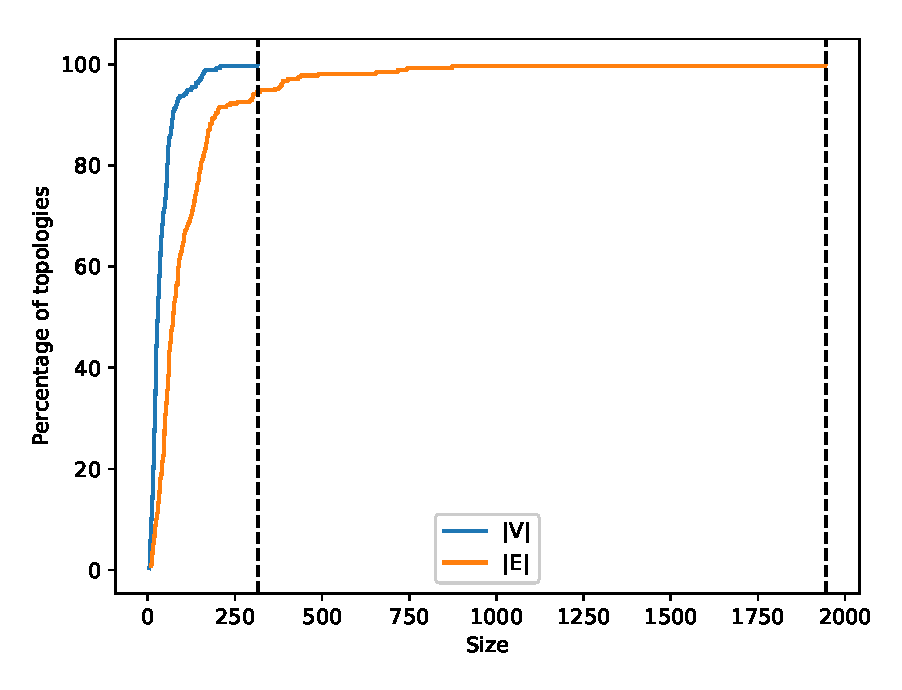
\includegraphics[width=.85\columnwidth]{./Network-lib/data/plot/topology_sizes.eps}
%\end{center}
%\caption{Distribution of the topology sizes.}
%\label{fig:sizes}
%\end{figure}

\begin{figure}
\begin{center}
\begin{tabular}{lrr}
\toprule
Topology name & $|V(G)|$ & $|E(G)|$\\
\midrule
AS 1221 & 104 & 302  \\
AS 1239 & 315 & 1944 \\
AS 1755 & 87 & 322   \\
AS 3257 & 161 & 656  \\
AS 3967 & 79 & 294   \\
AS 6461 & 138 & 744  \\
\bottomrule
\end{tabular}
\end{center}
\caption{Topology sizes in the \texttt{rf} group.}
\label{fig:rf_sizes}
\end{figure}

\begin{figure}
\begin{center}
\begin{tabular}{lrr}
\toprule
Topology name & $|V(G)|$ & $|E(G)|$\\
\midrule
ISP 1 & $\approx 150$ & $\approx 700$ \\
ISP 2 & $\approx 220$ & $\approx 800$ \\
ISP 3 & $\approx 170$ & $\approx 440$ \\
OVH   & 57 & 402 \\
\bottomrule
\end{tabular}
\end{center}
\caption{Topology sizes in the \texttt{real} group and \texttt{ovh}.}
\label{fig:real_sizes}
\end{figure}


\begin{figure}
\begin{center}
\begin{tabular}{lrr}
\toprule
Topology name & $|V(G)|$ & $|E(G)|$\\
\midrule
ITZ Cogentco  & 197 & 490 \\
ITZ Colt      & 153 & 382 \\
ITZ Deltacom  & 113 & 366 \\
ITZ Dia       & 138 & 302 \\
ITZ GtsCe     & 149 & 386 \\
ITZ Interoute & 110 & 312 \\
ITZ Ion       & 125 & 300 \\
ITZ Tata      & 145 & 388 \\
ITZ UsCarrier & 158 & 378 \\
\bottomrule
\end{tabular}
\end{center}
\caption{Largest topologies in the \texttt{zoo} group.}
\label{fig:zoo_sizes}
\end{figure}

\begin{figure}
\begin{center}
\begin{tabular}{cccc}
\toprule
Min $|V(G)|$ & Max $|V(G)|$ & Min $|E(G)|$ & Max $|E(G)|$ \\
\midrule
4 & 315 & 8 & 1955 \\
\bottomrule
\end{tabular}
\end{center}
\caption{Minimum and maximum topology sizes.}
\label{fig:sizes}
\end{figure}

\begin{figure}
\begin{center}
\begin{tabular}{cccc}
\toprule
Small & Medium & Large & Huge \\
$[0, 20]$ & $]20, 50]$ & $]50, 100]$ & $> 100$ \\
\midrule
30\% & 43\% & 21\% & 6\% \\
\bottomrule
\end{tabular}
\end{center}
\caption{Number of topologies by group size.}
\label{fig:group_sizes}
\end{figure}

\section{ECMP and non shortest path links}

We mentioned in the introduction that segment routing supports two kinds of segments: node segments 
and adjacency segments. We will see that adjacency segments are more costly and thus we would like to avoid using them whenever possible. However,
will see later that adjacency segments in segment routing can we necessary to implement paths that belong to ECMP components or that traverse
links that do not belong to any IGP shortest path. For that reason we analyzed the amount of ECMP component that exist in out dataset as well
as the amount of edges that do not belong to any shortest path. These values will give an estimation of how important supporting adjacency segments
is. Figure \ref{fig:ECMPcount} shows the percentage of links that do not belong to any shortest path as well as the percentage of pairs
of nodes with ECMP between them. We can see that, as expected, IGP weights are configured so that most links are used for shortest path routing, we
have only $1\%$ of the links falling outside of that.
We expect that mainly backup links will be configured so that they are not used unless a failure occurs. On the other hand, we see that
there is a relatively high percentage of pairs of nodes with ECMP. This indicates that adjacency segments will be useful whenever we want to
represent specific paths that traverse ECMP components. 

\begin{figure}
\begin{center}
\begin{tabular}{cccc}
\toprule
Links not in shortest paths & Pairs with ECMP \\
\midrule
$1\%$ & $26\%$  \\
\bottomrule
\end{tabular}
\end{center}
\caption{Percentage of links not in shortest paths and pairs with ECMP.}
\label{fig:ECMPcount}
\end{figure}

We also analyzed how many equal cost paths exist. Figure \ref{fig:ECMPcount} shows the CDF of the total number of shortest paths between each pair
of nodes over all topologies. This shows that some nodes are connected with a very high number of shortest paths but that most nodes have at most
$10$ shortest paths between them.

\begin{figure}
\begin{center}
\includegraphics[width=.85\columnwidth]{./Network-lib/data/plot/spCount.eps}
\end{center}
\caption{CDF over all topologies and all pairs of nodes of the number of shortest paths between those nodes.}
\label{fig:maxEDP_boxplot}
\end{figure}

\section{Degrees and density}

We also analyzed the degrees of the nodes in the topologies in our dataset as well as the edge densities. The degree of a router represents the
number of routers to which it tis connected to. It represents an upper bound on the number of edge-disjoint paths that can be used to
connect a given router to other routers. Figure \ref{fig:deg_boxplot} shows a box plot of these. We can observe that some nodes have a very
high degree but that the tendency is that most nodes have a degree lower than $10$. Nodes of degree $1$ are problematic in a network
because it means that there is a single point of failure to reach them. We observe that the largest topologies are the ones that suffer the least
from this problem.

\begin{figure}
\begin{center}
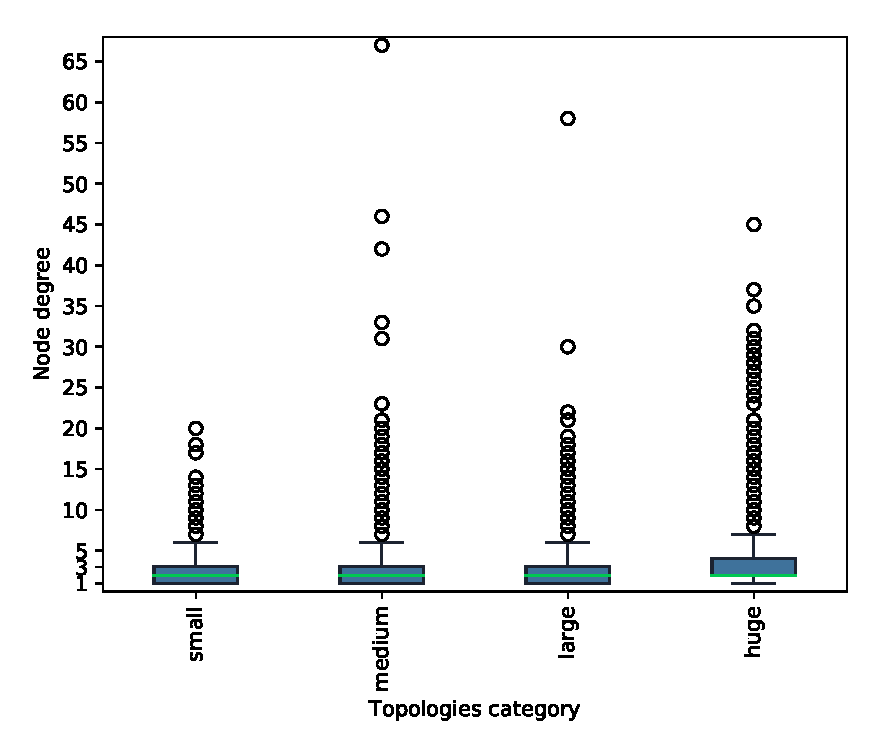
\includegraphics[width=.85\columnwidth]{./Network-lib/data/plot/deg_boxplot.eps}
\end{center}
\caption{Box plot of the degrees over the different size categories of our topologies.}
\label{fig:deg_boxplot}
\end{figure}

One degree nodes probably exist on these topologies due to the fact that most of them are were collected
using inexact methods thus leading to incomplete data. A computer network should at least be biconnected (have
at least two disjoint paths between every pair of nodes) to prevent a single link failure from partitioning
it.

The edge density of a network evaluates how close a network is from a complete graph. It is defined for graphs
with no parallel links as
$$
\frac{|E(G)|}{|V(G)| \cdot (|V(G)| - 1)}.
$$
A tree is the lowest density connected network that one can have. Any link failure in a tree will cause the network to become disconnected. High density network are costly but are more robust
to failures. They also provide a higher path diversity so optimal solution of network optimization problems tend to be
better on dense networks. Figure \ref{fig:density_cdf} shows a CDF of the densities over all topologies in
our dataset. We used the above formula even though some of our networks contain parallel links.
We can see that some network have a very low density. About $60\%$ percent of the network topologies
have an edge density of at least $10\%$ and $20\%$ of the networks have an edge density above $20\%$.

\begin{figure}
\begin{center}
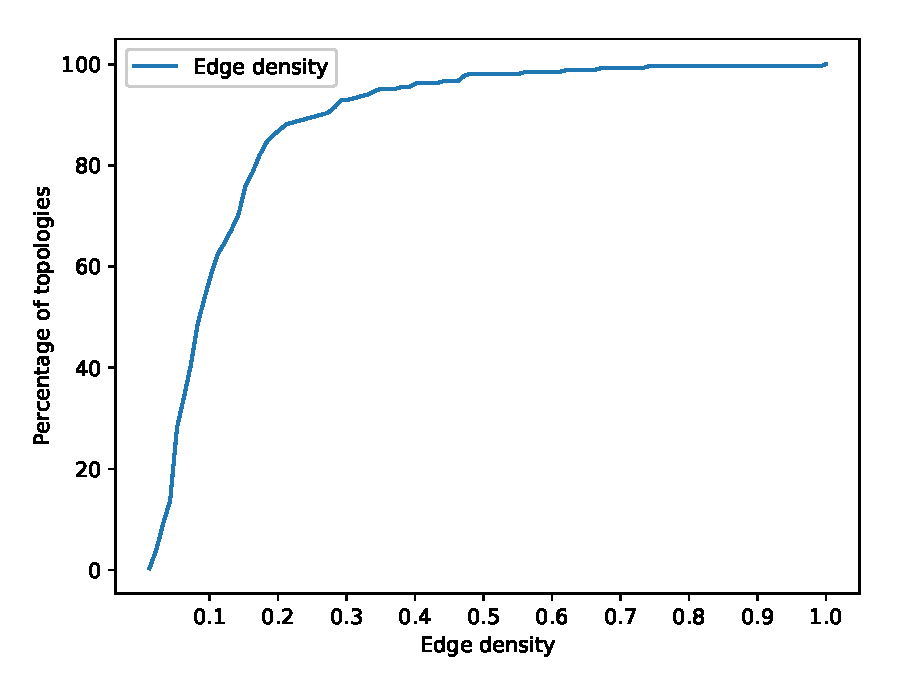
\includegraphics[width=.85\columnwidth]{./Network-lib/data/plot/edge_density.eps}
\end{center}
\caption{Box plot of the degrees over the different size categories of our topologies.}
\label{fig:density_cdf}
\end{figure}

\section{Connectivity}

We saw that some pairs of nodes have a lot of shortest paths between them. However these paths are of course not disjoint.
In this section we analyze how well the nodes are connected in the network. To measure this, we compute for each pair of nodes of each
topology the minimum number of links that need to be removed from the network in order to disconnect those nodes. This is known in graph
theory as the minimum cut between the nodes \cite{Ahuja}. Figure \ref{fig:mincut} shows a CDF of these minimum cuts. It is not hard to see
that the minimum cut between two nodes is the same as the maximum number of edge-disjoint paths between them \cite{Ahuja}.

\begin{figure}
\begin{center}
\includegraphics[width=.85\columnwidth]{./Network-lib/data/plot/minCuts.eps}
\end{center}
\caption{CDF over all topologies and all pairs of nodes of the number of shortest paths between those nodes.}
\label{fig:mincut}
\end{figure}

We can see that about $40\%$ of the pairs of nodes are connected by a single path as we had already observed above. This is quite low for a network as it does
not offer a lot of redundancy and link failures can easily disconnect the nodes. The remaining nodes require the removal of at least
$2$ links to disconnect them (in other words, they are in the same biconnected component \cite{Cormen:2009:IAT:1614191}). Also, nodes are very well connected having up to $46$ edge-disjoint paths connecting them.


\section*{Conclusion}

From this evaluation we observe that there is probably missing data on some of the topologies used in this
thesis as some of them are weakly connected. We have also seen that due to a high amout of ECMP ($26\%$) between pairs of nodes,
adjacency segments are likely to be necessary to implement paths in the graph topology with segment routing.

\chapter{Segment routing}
\label{chapter:sr}

\section*{Introduction}

As mentioned in the introduction, segment routing \cite{Filsfils_SR:2015} is a new forwarding architecture that is being developed within the Internet Engineering Task Force and network operators.
Segment Routing changes the way packets are forwarded
inside a network to enable network operators to have better
control on the path followed by the packets. Traffic can be forced to follow a series of detours
which can either correspond to passing by a specific router or network link.

This chapter is dedicated to formalizing segment routing. We provide, to the best of our knowledge, the first formalization that comprises
both node and adjacency segments. We define minimal segmentations and provide an efficient algorithm for computing 
them. We also provide reachability concepts which allow to analyze the capability of a given network topology
to support segment routing as well as giving lower bound on the minimum number of segments needed reach every single link
in the network. These concepts will be fundamental later on when we propose an algorithm for computing cycle covers 
of a network.

% Figure \ref{fig:srformal_sr1} illustrates an example of SR. In this example the ingress node is node 
% $\node{a}$ and there are two segments in the SR stack: an adjacent segment representing link $(\node{d}, \node{e})$
% and a node segment representing node $\node{i}$. We assume in the figure that all IGP weights are
% equal to $1$. The ingress node will look at the segment on the top of the stack and find link
% $(\node{d}, \node{e})$. It will then forward the packet to trough origin of the link, node $\node{d}$, through the shortest
% path $(\node{a}, \node{c}, \node{d})$. Then node $\node{d}$ will receive it an forward it to $\node{e}$ one the link $(\node{d}, \node{e})$.
% Node $\node{e}$ will then examine the segment stack see that the next segment is node $\node{i}$. It then
% forwards the packet to node $\node{i}$ via the shortest path $(\node{e}, \node{h}, \node{i})$.
% 
% \begin{figure}[H]
% \begin{center}
% \begin{tikzpicture}
% \def\x{0}
% \def\y{0}
% \node[scale=0.15] (a) at (0.5 + \x,  0.5 + \y) {\router{a}{green}};
% \node[scale=0.15] (b) at (0.5 + \x, -1.0 + \y) {\router{b}{lightgray}};
% \node[scale=0.15] (c) at (2.5 + \x,  0.0 + \y) {\router{c}{lightgray}};
% \node[scale=0.15] (d) at (4.5 + \x,  0.0 + \y) {\router{d}{green}};
% \node[scale=0.15] (e) at (4.0 + \x, -2.0 + \y) {\router{e}{green}};
% \node[scale=0.15] (g) at (6.0 + \x,  0.5 + \y) {\router{g}{lightgray}};
% \node[scale=0.15] (i) at (8.0 + \x,  0.0 + \y) {\router{i}{green}};
% \node[scale=0.15] (h) at (7.0 + \x, -1.5 + \y) {\router{h}{lightgray}};
% \node[scale=0.15] (f) at (4.0 + \x, -3.5 + \y) {\router{f}{lightgray}};
% \node[scale=0.15] (j) at (8.0 + \x, -2.5 + \y) {\router{j}{lightgray}};
% \draw[line width=2] (f) edge[above, sloped] node[black,font=\bfseries] {\tiny \texttt{}} (j);
% \draw[line width=2] (h) edge[above, sloped] node[black,font=\bfseries] {\tiny \texttt{}} (j);
% \draw[line width=2] (a) edge[above, sloped] node[black,font=\bfseries] {\tiny \texttt{}} (b);
% \draw[line width=2] (b) edge[above, sloped] node[black,font=\bfseries] {\tiny \texttt{}} (c);
% \draw[line width=2] (e) edge[above, sloped] node[black,font=\bfseries] {\tiny \texttt{}} (c);
% \draw[line width=2] (b) edge[above, sloped] node[black,font=\bfseries] {\tiny \texttt{}} (e);
% \draw[line width=2] (b) edge[above, sloped] node[black,font=\bfseries] {\tiny \texttt{}} (f);
% \draw[line width=2] (e) edge[above, sloped] node[black,font=\bfseries] {\tiny \texttt{}} (f);
% \draw[line width=2] (h) edge[above, sloped] node[black,font=\bfseries] {\tiny \texttt{}} (f);
% \draw[line width=2] (g) edge[above, sloped] node[black,font=\bfseries] {\tiny \texttt{}} (i);
% \draw[line width=2] (i) edge[above, sloped] node[black,font=\bfseries] {\tiny \texttt{}} (h);
% \draw[line width=2]  (d) edge[above, sloped] node[black,font=\bfseries] {\tiny \texttt{}} (g);
% \draw[line width=2]  (d) edge[above, sloped] node[black,font=\bfseries] {\tiny \texttt{}} (e);
% \draw[line width=2]  (e) edge[above, sloped] node[black,font=\bfseries] {\tiny \texttt{}} (h);
% \draw[line width=2]  (g) edge[above, sloped] node[black,font=\bfseries] {\tiny \texttt{}} (h);
% \draw[line width=2]  (c) edge[above, sloped] node[black,font=\bfseries] {\tiny \texttt{}} (d);
% \draw[line width=2]  (a) edge[above, sloped] node[black,font=\bfseries] {\tiny \texttt{}} (b);
% \draw[line width=2]  (a) edge[above, sloped] node[black,font=\bfseries] {\tiny \texttt{}} (c);
% 
% %%%%
% \draw (a) edge[line width=2, darkgreen, above, ->, bend right = 20] (c);
% \draw (c) edge[line width=2, darkgreen, above, ->, bend right = 20] (d);
% \draw (d) edge[line width=2, darkgreen, above, ->, dotted] (e);
% \draw (e) edge[line width=2, darkgreen, above, ->, bend left = 20] (h);
% \draw (h) edge[line width=2, darkgreen, above, ->, bend left = 20] (i);
% 
% 
% \def\x{-0.25}
% \def\y{1}
% \node at (\x + 2.2, \y + 0.25) {\footnotesize SR stack};
% \fill[lightgray] (\x, \y) rectangle (\x + 1.5, \y + 0.5);
% \fill[green] (\x, \y) rectangle (\x + 1, \y + 0.5);
% \draw[dotted, thick] (\x + 0.4, \y) -- (\x + 0.4, \y - 0.4);
% \draw[] (\x, \y) rectangle (\x + 1, \y + 0.5);
% \draw[] (\x, \y) rectangle (\x + 1.5, \y + 0.5);
% \draw (\x + 1, \y) -- (\x + 1, \y + 0.5);
% \node at (\x + 0.5, \y + 0.25) {\footnotesize $(d, e)$};
% \node at (\x + 1.25, \y + 0.28) {\footnotesize $i$};
% 
% \def\x{3.25}
% \def\y{-3}
% \fill[gray] (\x, \y) rectangle (\x + 1.5, \y + 0.5);
% \fill[green] (\x + 1, \y) rectangle (\x + 1.5, \y + 0.5);
% \draw[dotted, thick] (\x + 0.4, \y + 0.8) -- (\x + 0.4, \y + 0.5);
% \draw[] (\x, \y) rectangle (\x + 1, \y + 0.5);
% \draw[] (\x, \y) rectangle (\x + 1.5, \y + 0.5);
% \draw (\x + 1, \y) -- (\x + 1, \y + 0.5);
% \node at (\x + 0.5, \y + 0.25) {\footnotesize $(d, e)$};
% \node at (\x + 1.25, \y + 0.28) {\footnotesize $i$};
% 
% 
% \def\x{8 - 0.75}
% \def\y{0.5}
% \fill[gray] (\x, \y) rectangle (\x + 1.5, \y + 0.5);
% \draw[dotted, thick] (\x + 0.4, \y) -- (\x + 0.4, \y - 0.4);
% \draw[] (\x, \y) rectangle (\x + 1, \y + 0.5);
% \draw[] (\x, \y) rectangle (\x + 1.5, \y + 0.5);
% \draw (\x + 1, \y) -- (\x + 1, \y + 0.5);
% \node at (\x + 0.5, \y + 0.25) {\footnotesize $(d, e)$};
% \node at (\x + 1.25, \y + 0.28) {\footnotesize $i$};
% 
% 
% %%%%
% 
% %\def\x{-1}
% 
% %\draw[line width=2] (\x + 10, \y + -1 + 0.5) edge[] (\x + 10.5, \y + -1 + 0.5);
% %\node[anchor=west]  at (\x + 10.5, \y + -1 + 0.5) {\footnotesize network link};
% 
% %\draw[line width=2] (\x + 10, \y + -1) edge[dotted, darkgreen, ->] (\x + 10.5, \y + -1);
% %\node[anchor=west]  at (\x + 10.5, \y + -1) {\footnotesize adjacency segment};
% 
% %\draw[line width=2] (\x + 10, \y + -1 - 0.5) edge[] (\x + 10.5, \y + -1 - 0.5);
% %\node[anchor=west]  at (\x + 10.5, \y + -1 - 0.5) {\footnotesize s link};
% 
% 
% \end{tikzpicture}
% \end{center}
% \caption{Illustration of SR with segments $(d, e)$ and $i$ and ingress node $a$. Dashed arrows represent adjacency segments
% and the others represent the shortest path edges between consecutive segments.}
% \label{fig:srformal_sr1}
% \end{figure}
% 
% This chapter is organized as follows. We start in Section \ref{section:sr-formal} by providing a formalization
% of segment routing. To the best of our knowledge, this is the first work that studies segment routing in
% 
% \todo{finish chapter organization}
% 
% \todo{we need to explain that when the graph is undirected we don't draw both arrows}


\section{Segment routing formalization}

\label{section:sr-formal}

The starting point of our segment routing formalization is the concept of segment routing path, or sr-path for short.

\begin{definition}
Let $G$ be a network. A \emph{sr-path} $\sr{p}$ on $G$ is a sequence $\langle x_1, \ldots, x_l \rangle$ such that each $x_i \in V(G) \cup E(G)$.
%We use the notation $\sr{p}_i = x_i$ to represent the $i$-th element in the sequence.
\end{definition}

We represent sr-paths with the vector notation to be able to more easily distinguish between a path $p$ and a 
sr-path $\sr{p}$ in the network $G$. In practice, the elements of $\sr{p}$ that are nodes model node segments and
the elements of $\sr{p}$ that are edges model adjacency segments. It is important to understand that, because of ECMP, a sr-path
actually can correspond to a set of paths in the original network. 

Consider the sr-path $\sr{p} = \langle \node{a}, \node{c}, \node{e}, (\node{f}, \node{j}), \node{i} \rangle$ shown in
Figure \ref{fig:sr-path}. The solid green edges show the set of edges that belong to shortest paths between consecutive segments
and the dashed green edge represents the adjacency segment $(\node{f}, \node{j})$. The square boxes represent segments. The box is represented next to
a node for node segments and on top of the link of an adjacency segment. So, in this case, $x_1 = \node{a}, x_2 = \node{c}, x_3 = \node{e}, x_4 = \edge{f}{j}$
and $x_5 = \node{i}$.

In this example, between nodes \node{c} and \node{e} there are two shortest paths, namely
$((\node{c}, \node{d}), (\node{d}, \node{e}))$ and $((\node{c}, \node{b}), (\node{b}, \node{e}))$. In the same way,
two shortest paths exist between nodes \node{e} and \node{f} because we have two parallel links with the same IGP weight
between them. In each case, any of those two paths could be used to forward packets over this
sr-path. Thus, we see that the sr-path $\sr{p}$ can correspond to four paths over the original network, namely,

\begin{align*}
((\node{a}, \node{c}), (\node{c}, \node{d}), (\node{d}, \node{e}), (\node{e}, \node{f}, i_1), (\node{f}, \node{j}), (\node{j}, \node{h}), (\node{h}, \node{i})), \\
((\node{a}, \node{c}), (\node{c}, \node{d}), (\node{d}, \node{e}), (\node{e}, \node{f}, i_2), (\node{f}, \node{j}), (\node{j}, \node{h}), (\node{h}, \node{i})), \\
((\node{a}, \node{c}), (\node{c}, \node{b}), (\node{b}, \node{e}), (\node{e}, \node{f}, i_1), (\node{f}, \node{j}), (\node{j}, \node{h}), (\node{h}, \node{i})), \\
((\node{a}, \node{c}), (\node{c}, \node{b}), (\node{b}, \node{e}), (\node{e}, \node{f}, i_2), (\node{f}, \node{j}), (\node{j}, \node{h}), (\node{h}, \node{i})) \\
\end{align*}

where $(\node{e}, \node{f}, i_1)$ and $(\node{e}, \node{f}, i_2)$ represent the two links between $\node{e}$ and $\node{f}$.

\begin{figure}
\begin{center}
\begin{tikzpicture}
\def\x{0}
\def\y{0}
\node[scale=0.15] (a) at (0.5 + \x,  0.5 + \y) {\router{a}{marked}};
\node[scale=0.15] (b) at (0.5 + \x, -1.0 + \y) {\router{b}{router}};
\node[scale=0.15] (c) at (2.5 + \x,  0.0 + \y) {\router{c}{marked}};
\node[scale=0.15] (d) at (4.5 + \x,  0.0 + \y) {\router{d}{router}};
\node[scale=0.15] (e) at (4.0 + \x, -2.0 + \y) {\router{e}{marked}};
\node[scale=0.15] (g) at (6.0 + \x,  0.5 + \y) {\router{g}{router}};
\node[scale=0.15] (i) at (8.0 + \x,  0.0 + \y) {\router{i}{marked}};
\node[scale=0.15] (h) at (7.0 + \x, -1.5 + \y) {\router{h}{router}};
\node[scale=0.15] (f) at (4.0 + \x, -3.5 + \y) {\router{f}{router}};
\node[scale=0.15] (j) at (8.0 + \x, -2.5 + \y) {\router{j}{router}};
\draw[line width=2] (f) edge[above, sloped] node[black,font=\bfseries] {\tiny \texttt{}} (j);
\draw[line width=2] (h) edge[above, sloped] node[black,font=\bfseries] {\tiny \texttt{}} (j);
\draw[line width=2] (a) edge[above, sloped] node[black,font=\bfseries] {\tiny \texttt{}} (b);
\draw[line width=2] (b) edge[above, sloped] node[black,font=\bfseries] {\tiny \texttt{}} (c);
\draw[line width=2] (b) edge[above, sloped] node[black,font=\bfseries] {\tiny \texttt{}} (e);
\draw[line width=2] (b) edge[above, sloped] node[black,font=\bfseries] {\tiny \texttt{}} (f);
\draw[line width=2] (e) edge[above, sloped, bend left=10] node[black,font=\bfseries] {\tiny \texttt{}} (f);
\draw[line width=2] (e) edge[above, sloped, bend right=10] node[black,font=\bfseries] {\tiny \texttt{}} (f);
\draw[line width=2] (h) edge[above, sloped] node[black,font=\bfseries] {\tiny \texttt{}} (f);
\draw[line width=2] (g) edge[above, sloped] node[black,font=\bfseries] {\tiny \texttt{}} (i);
\draw[line width=2] (i) edge[above, sloped] node[black,font=\bfseries] {\tiny \texttt{}} (h);
\draw[line width=2]  (d) edge[above, sloped] node[black,font=\bfseries] {\tiny \texttt{}} (g);
\draw[line width=2]  (d) edge[above, sloped] node[black,font=\bfseries] {\tiny \texttt{}} (e);
\draw[line width=2]  (e) edge[above, sloped] node[black,font=\bfseries] {\tiny \texttt{}} (h);
\draw[line width=2]  (g) edge[above, sloped] node[black,font=\bfseries] {\tiny \texttt{}} (h);
\draw[line width=2]  (c) edge[above, sloped] node[black,font=\bfseries] {\tiny \texttt{}} (d);
\draw[line width=2]  (a) edge[above, sloped] node[black,font=\bfseries] {\tiny \texttt{}} (b);
\draw[line width=2]  (a) edge[above, sloped] node[black,font=\bfseries] {\tiny \texttt{}} (c);

%%%%
\draw (a) edge[line width=3, darkgreen, above, ->, bend left = 20] (c);
\draw (c) edge[line width=3, darkgreen, above, ->, bend right = 20] (d);
\draw (c) edge[line width=3, darkgreen, above, ->, bend right = 20] (b);
\draw (b) edge[line width=3, darkgreen, above, ->, bend left = 20] (e);
\draw (d) edge[line width=3, darkgreen, above, ->, bend right = 20] (e);

\draw (j) edge[line width=3, darkgreen, above, ->, bend left = 20] (h);
\draw (f) edge[line width=4, darkgreen, ->, dotted] node[line width = 1, draw, solid, black, fill=green] {\footnotesize $x_4$} (j);

\draw (h) edge[line width=3, darkgreen, above, ->, bend left = 20] (i);
\draw (e) edge[line width=3, darkgreen, above, ->, bend right = 30] (f);
\draw (e) edge[line width=3, darkgreen, above, ->, bend left = 30] (f);

\node[left = 0.1cm of a, draw, fill=green] {\footnotesize $x_1$};
\node[above = 0.1cm of c, draw, fill=green] {\footnotesize $x_2$};
\node[above right = 0.1cm of e, draw, fill=green] {\footnotesize $x_3$};
\node[right = 0.1cm of i, draw, fill=green] {\footnotesize $x_4$};

\end{tikzpicture}
\end{center}
\caption{Illustration of sr-path $\sr{p} = \langle \node{a}, \node{c}, \node{e}, (\node{f}, \node{j}), \node{i} \rangle$.}
\label{fig:sr-path}
\end{figure}


In general, when we use a sr-path $\sr{p} = \langle x_1, \ldots, x_l \rangle$ to forward traffic, between segments $x_i$ and $x_{i + 1}$ the set of paths
over which this traffic might be sent corresponds to the set of all shortest paths between those segments. In this thesis we consider two models for
forwarding traffic over ECMP:

\begin{enumerate}
 \item \emph{Hash model}: Whenever several next-hops exists with respect to the IGP shortest paths, a hash function is used to select which of them is used.
 This hash function is unknown and depends on the traffic that is sent. From a practical point of view this, more or less, corresponds to assuming that one of the
 multiple shortest paths is selected at random.
 
 \item \emph{Split model}: The traffic is split evenly between all shortest paths. This means that if, for instance, a router contains two next-hops, it will forward
 $50\%$ of the traffic towards one of them and the other $50\%$ towards the other.
\end{enumerate}


But these segments, $x_i$ and $x_{i + 1}$ might not both correspond to nodes in which case we need to give a precise definition of what the set of shortest paths between two segments means. 
In general, we have four cases which are summarized
in Figure \ref{fig:4case-sr}. If we have two node segments $x_i = v, x_{i + 1} = u$ then it is the subgraph between $v$ and $u$, $\sp(v, u)$. 
If $x_i = v$ and $x_{i + 1} = (u_1, u_2)$ then it the subgraph between $v$ and $u_1$, $\sp(v, u_1)$. If $x_i = (v_1, v_2)$ and $x_{i + 1} = u$ then it is
the shortest path subgraph between $v_2$ and $u$. Finally, if both are adjacency segments with $x_i = (v_1, v_2)$ and $x_{i + 1} = (u_1, u_2)$ then it is
$\sp(v_2, u_1)$.

\begin{figure}[H]
\begin{center}
\begin{tabular}{c}
\begin{tikzpicture}
\node[scale=0.15] (v) at (0, 0) {\router{$v$}{marked}};
\node[scale=0.15] (u) at (3, 0) {\router{$u$}{marked}};
\path (v) edge[line width=2, darkgreen, out=-30, in=240, wavy, ->] (u);
\path (v) edge[line width=2, darkgreen, out=30, in=150, wavy, ->] (u);
\node at (0, 1) {$x_i = v$};
\node at (3, 1) {$x_{i+1} = u$};
\node[darkgreen,font=\bfseries] at (1.5, 0) {$\sp(v, u)$};
\end{tikzpicture}
\\
\emph{Case 1:} $x_i$ and $x_{i + 1}$ are both node segments
\\[0.5cm]
\begin{tikzpicture}
\node[scale=0.15] (v) at (0, 0) {\router{$v$}{marked}};
\node[scale=0.15] (u1) at (3, 0) {\router{$u_1$}{router}};
\node[scale=0.15] (u2) at (5, 0) {\router{$u_2$}{router}};
\path (v) edge[line width=2, darkgreen, out=-30, in=240, wavy, ->] (u1);
\path (v) edge[line width=2, darkgreen, out=30, in=150, wavy, ->] (u1);
\draw[line width=2]  (u1) edge[above, sloped] node[black,font=\bfseries] (l) {} (u2);
\draw (u1) edge[line width=4, darkgreen, above, ->, dotted] (u2);
\node at (0, 1) {$x_i = v$};
\node at (4, 1) {$x_{i+1} = (u_1, u_2)$};
\node[darkgreen,font=\bfseries] at (1.5, 0) {$\sp(v, u_1)$};
\end{tikzpicture}
\\
\emph{Case 2:} $x_i$ is a node segment and $x_{i + 1}$ is an adjacency segment
\\[0.5cm]
\begin{tikzpicture}
\node[scale=0.15] (v1) at (0, 0) {\router{$v_1$}{router}};
\node[scale=0.15] (v2) at (2, 0) {\router{$v_2$}{router}};
\node[scale=0.15] (u) at (5, 0) {\router{$u$}{marked}};
\path (v2) edge[line width=2, darkgreen, out=-30, in=240, wavy, ->] (u);
\path (v2) edge[line width=2, darkgreen, out=30, in=150, wavy, ->] (u);
\draw[line width=2]  (v1) edge[above, sloped] node[black,font=\bfseries] (l) {} (v2);
\draw (v1) edge[line width=4, darkgreen, above, ->, dotted] (v2);
\node at (1, 1) {$x_i = (v_1, v_2)$};
\node at (5, 1) {$x_{i+1} = u$};
\node[darkgreen,font=\bfseries] at (3.5, 0) {$\sp(v_2, u)$};
\end{tikzpicture}
\\
\emph{Case 3:} $x_i$ is an adjacency segment and $x_{i + 1}$ is a node segment
\\[0.5cm]
\begin{tikzpicture}
\node[scale=0.15] (v1) at (0, 0) {\router{$v_1$}{router}};
\node[scale=0.15] (v2) at (2, 0) {\router{$v_2$}{router}};
\node[scale=0.15] (u1) at (5, 0) {\router{$u_1$}{router}};
\node[scale=0.15] (u2) at (7, 0) {\router{$u_2$}{router}};
\path (v2) edge[line width=2, darkgreen, out=-30, in=240, wavy, ->] (u1);
\path (v2) edge[line width=2, darkgreen, out=30, in=150, wavy, ->] (u1);
\draw[line width=2]  (v1) edge[above, sloped] node[black,font=\bfseries] (l) {} (v2);
\draw (v1) edge[line width=4, darkgreen, above, ->, dotted] (v2);
\draw[line width=2]  (u1) edge[above, sloped] node[black,font=\bfseries] (l) {} (u2);
\draw (u1) edge[line width=4, darkgreen, above, ->, dotted] (u2);
\node at (1, 1) {$x_i = (v_1, v_2)$};
\node at (6, 1) {$x_{i+1} = (u_1, u_2)$};
\node[darkgreen,font=\bfseries] at (3.5, 0) {$\sp(v_2, u_1)$};
\end{tikzpicture}
\\
\emph{Case 4:} $x_i$ and $x_{i + 1}$ are both adjacency segments
\end{tabular}
\end{center}
\caption{Shortest paths between consecutive segments.}
\label{fig:4case-sr}
\end{figure}

Having to deal with these four cases would be very cumbersome. When considering a sr-path $\sr{p}$ we want to have a way to
ignore as much as possible the nature of each of the segments. This will make proving results involving sr-paths easier and also
will ease the readability of proofs. This lead us to define the following notation so that we can
very simply capture all four cases.

\begin{definition}
Let $G$ be a network and $\sr{p} = \langle x_1, \ldots, x_l \rangle$. If $x_i \in V(G)$ we define $x^1_i = x^2_i = x_i$ and
if $x_i = (u_1, u_2) \in E(G)$ we define $x^1_i = u_1$ and $x^2_i = u_2$. 
\end{definition}

With this notation, we can now simply say that the set of shortest paths between two consecutive segments $x_i$ and $x_{i + 1}$
of a sr-path $\sr{p}$ is the subgraph $\sp(x^2_i, x^1_{i + 1})$. This works regardless of what the type of segments $x_i$ and $x_{i + 1}$
are. This notation also makes it easy to refer to the starting and ending routers of a sr-path.

\begin{definition}
Let $G$ be a network and $\sr{p} = \langle x_1, \ldots, x_l \rangle$. We say that $\sr{p}$ is a sr-path from node $x^1_1$ to
$x^2_l$. We say that $x^1_1$ is the first node of $\sr{p}$ and $x^2_l$ is the last node of $\sr{p}$. A sr-path that
starts and ends at the same node is called a sr-cycle.
\end{definition}

As we mentioned in the introduction of this chapter, when we use segment routing as a forwarding mechanism, we need to append to the packet 
header the segments that are to be used. Commercial routers have strong limitations regarding the size of this header. Some routers can
support sr-paths with up to $10$ segments but on average this number is closer to $5$ \cite{Tantsura_SID:2017}.
This means that it is important to be able to capture the cost, in terms of segments, of a sr-path. A node segment needs to contain
the IP address of the corresponding router whereas an adjacency segment needs the IP address of the source node of the corresponding link
as well as the interface identifier of that link. For this reason, we model the cost of individual segments and sr-paths as follows.

\begin{definition}
Let $G$ be a network and $\sr{p} = \langle x_1, \ldots x_l \rangle$ a sr-path on $G$. We define the cost of $x_i$ as
\[ \cost(x_i) =
  \begin{cases}
    1 & \quad \text{if } x_{i} \in V(G) \\
    2 & \quad \text{otherwise}
  \end{cases}
\]
We define the \emph{segment cost} of $\sr{p}$ as
$$
\cost(\sr{p}) = \sum_{i = 1}^l \cost(x_i)
$$
\end{definition}

Note that this model does not exactly match the reality. In practice, if the first segment is a node segment, its IP address will never be put into the
segment stack. Also, if the first segment is an adjacency segment only the link interface would be necessary
for the same reason. We chose to ignore this and count each segment equally because it greatly simplifies the mathematical developments. Furthermore, we
believe that the model is close enough that this will have a minor impact in practice. In the worst case, we overestimate the real segment cost
of a sr-path by $1$.

\begin{definition}
Let $G$ be a network. We denote the set of all sr-paths on $G$ by $\sr{\mathcal{P}}$. Given $k \in \mathbb{N}$ we define
$$
\mathcal{\sr{P}}_k(G) = \left\{ \sr{p} \mid \text{$\sr{p}$ is a sr-path on $G$ and $\cost(\sr{p}) \leq k$} \right\}.
$$
Finally, given $s, t \in V(G)$ we denote the set of all sr-paths from $s$ to $t$ of segment cost at most $k$
by $\Pk(s, t)$.

\end{definition}

We now define some operations on sr-paths and prove some of theirs properties.
 
\begin{definition}
Let $G$ be a network and $\sr{p} = \langle x_1, \ldots, x_l \rangle, \sr{q} = \langle y_1, \ldots, y_r \rangle$ be two sr-paths on $G$. We 
define the sum of $\sr{p}$ and $\sr{q}$ as
$$
\sr{p} + \sr{q} = \langle x_1, \ldots, x_l, y_1, \ldots, y_r \rangle
$$
\end{definition}

\begin{lemma}
\label{lemma:srsumcost}
Let $G$ be a network and $\sr{p} = \langle x_1, \ldots, x_l \rangle, \sr{q} = \langle y_1, \ldots, y_r \rangle$ be two sr-paths on $G$. Then
$$
\cost(\sr{p} + \sr{q}) = \cost(\sr{p}) + \cost(\sr{q}) 
$$
\end{lemma}

\begin{proof}
\begin{align*}
\cost(\sr{p} + \sr{q}) & = \cost(\langle x_1, \ldots, x_l, y_1, \ldots, y_r) \\
& = \sum_{i = 1}^l \cost(x_i) + \sum_{i = 1}^r \cost(y_i) \\
& = \cost(\sr{p}) + \cost(\sr{q})
\end{align*}
\end{proof}

Addition of sr-paths will turn out to be useful to prove
bounds on the segment cost of sr-paths produced by some of our algorithms. However, 
addition of sr-paths does not care about the segments contained in each path. It simply takes all segments
from both paths and put them in order into a single sr-path. For example, it could be the case that $x_l = y_1$
so the resulting sr-path would have a segment repeated twice next to each other. This does not 
cause any practical problem but in terms of routing it is redundant. Moreover, it wastes space in the segment stack. This can be the case even if $x_l \neq y_1$ but the last node of $x_l$ and the first node of $y_1$ 
are the same, that is, if $x^2_l = y^1_1$. For instance let $\sr{p} = \langle \node{a}, \node{f} \rangle$ and
$\sr{q} = \langle (\node{f}, \node{j}), \node{i} \rangle$. Then 
$\sr{p} + \sr{q} = \langle \node{a}, \node{f}, (\node{f}, \node{j}), \node{i} \rangle$. 
In terms of routing, this sr-path traverses the same links as the sr-path $\langle \node{a}, (\node{f}, \node{j}), \node{i} \rangle$
but it costs one more because it has a useless node segment on $\node{f}$.
With this in mind, we define a concatenation operation $\oplus$ on sr-paths which takes this into account and discards useless segments at the concatenation
point in the resulting sr-path.

% \begin{figure}[H]
% \begin{center}
% \begin{tikzpicture}
% \def\x{0}
% \def\y{0}
% \node[scale=0.15] (a) at (0.5 + \x,  0.5 + \y) {\router{a}{green}};
% \node[scale=0.15] (b) at (0.5 + \x, -1.0 + \y) {\router{b}{router}};
% \node[scale=0.15] (c) at (2.5 + \x,  0.0 + \y) {\router{c}{router}};
% \node[scale=0.15] (d) at (4.5 + \x,  0.0 + \y) {\router{d}{router}};
% \node[scale=0.15] (e) at (4.0 + \x, -2.0 + \y) {\router{e}{router}};
% \node[scale=0.15] (g) at (6.0 + \x,  0.5 + \y) {\router{g}{router}};
% \node[scale=0.15] (i) at (8.0 + \x,  0.0 + \y) {\router{i}{green}};
% \node[scale=0.15] (h) at (7.0 + \x, -1.5 + \y) {\router{h}{router}};
% \node[scale=0.15] (f) at (4.0 + \x, -3.5 + \y) {\router{f}{green}};
% \node[scale=0.15] (j) at (8.0 + \x, -2.5 + \y) {\router{j}{green}};
% \draw[line width=2] (f) edge[above, sloped] node[black,font=\bfseries] {\tiny \texttt{}} (j);
% \draw[line width=2] (h) edge[above, sloped] node[black,font=\bfseries] {\tiny \texttt{}} (j);
% \draw[line width=2] (a) edge[above, sloped] node[black,font=\bfseries] {\tiny \texttt{}} (b);
% \draw[line width=2] (b) edge[above, sloped] node[black,font=\bfseries] {\tiny \texttt{}} (c);
% \draw[line width=2] (b) edge[above, sloped] node[black,font=\bfseries] {\tiny \texttt{}} (e);
% \draw[line width=2] (b) edge[above, sloped] node[black,font=\bfseries] {\tiny \texttt{}} (f);
% \draw[line width=2] (e) edge[above, sloped, bend left=10] node[black,font=\bfseries] {\tiny \texttt{}} (f);
% \draw[line width=2] (e) edge[above, sloped, bend right=10] node[black,font=\bfseries] {\tiny \texttt{}} (f);
% \draw[line width=2] (h) edge[above, sloped] node[black,font=\bfseries] {\tiny \texttt{}} (f);
% \draw[line width=2] (g) edge[above, sloped] node[black,font=\bfseries] {\tiny \texttt{}} (i);
% \draw[line width=2] (i) edge[above, sloped] node[black,font=\bfseries] {\tiny \texttt{}} (h);
% \draw[line width=2]  (d) edge[above, sloped] node[black,font=\bfseries] {\tiny \texttt{}} (g);
% \draw[line width=2]  (d) edge[above, sloped] node[black,font=\bfseries] {\tiny \texttt{}} (e);
% \draw[line width=2]  (e) edge[above, sloped] node[black,font=\bfseries] {\tiny \texttt{}} (h);
% \draw[line width=2]  (g) edge[above, sloped] node[black,font=\bfseries] {\tiny \texttt{}} (h);
% \draw[line width=2]  (c) edge[above, sloped] node[black,font=\bfseries] {\tiny \texttt{}} (d);
% \draw[line width=2]  (a) edge[above, sloped] node[black,font=\bfseries] {\tiny \texttt{}} (b);
% \draw[line width=2]  (a) edge[above, sloped] node[black,font=\bfseries] {\tiny \texttt{}} (c);
% 
% %%%%
% \draw (a) edge[line width=3, darkgreen, above, ->, bend right = 20] (b);
% \draw (b) edge[line width=3, darkgreen, above, ->, bend right = 20] (f);
% 
% \draw (j) edge[line width=3, darkgreen, above, ->, bend left = 20] (h);
% \draw (f) edge[line width=4, darkgreen, above, ->, dotted] (j);
% 
% \draw (h) edge[line width=3, darkgreen, above, ->, bend left = 20] (i);
% 
% \end{tikzpicture}
% \end{center}
% \label{fig:sr-add}
% \caption{Illustration of sr-path $\sr{p} + \sr{q} = \langle \node{a}, \node{f} \rangle + \langle (\node{f}, \node{j}), \node{i} \rangle = \langle \node{a}, \node{f}, (\node{f}, \node{j}), \node{i} \rangle$.}
% \end{figure}

\begin{definition}
\label{def:sr-concat}
Let $G$ be a network and $\sr{p} = \langle x_1, \ldots, x_l \rangle$ be a sr-path from
$a$ to $b$ and $\sr{q} = \langle y_1, \ldots, y_r \rangle$ be a sr-path from $b$ to $c$, where $a, b, c \in V(G)$.
We  define the concatenation of $\sr{p}$ and $\sr{q}$ as
\[ \sr{p} \oplus \sr{q} =
  \begin{cases}
    \langle x_1, \ldots, x_l, y_2, \ldots, y_r \rangle & \quad \text{if } x_l = y_1 = b \in V(G) \\
    \langle x_1, \ldots, x_l, y_2, \ldots, y_r \rangle & \quad \text{if } x_l \in E(G) \text{ and } y_1 \in V(G) \\
    \langle x_1, \ldots, x_{l - 1}, y_1, \ldots, y_r \rangle & \quad \text{if } x_l \in V(G) \text{ and } y_1 \in E(G) \\
    \langle x_1, \ldots, x_l, y_1, \ldots, y_r \rangle & \quad \text{if } x_l \in E(G) \text{ and } y_1 \in E(G) \\
  \end{cases}
\]
\end{definition}

With sr-path concatenation we avoid consecutive redundant segments by removing them if necessary beforehand.
For the above example with $\sr{p} = \langle \node{a}, \node{f} \rangle$ and
$\sr{q} = \langle (\node{f}, \node{j}), \node{i} \rangle$ we have 
$\sr{p} \oplus \sr{q} = \langle \node{a}, (\node{f}, \node{j}), \node{i} \rangle$. Figure \ref{fig:sr-concat}
illustrates the four cases of sr-path concatenation from Definition \ref{def:sr-concat}.

\begin{figure}[H]
\begin{center}
\begin{tabular}{c}
\begin{tikzpicture}
\draw[cyan, ultra thick] (-3.5, -0.5) rectangle (0.6, 0.5);
\draw[orange, ultra thick] (1.4, -0.5) rectangle (5.5, 0.5);

\node[scale=0.15] (v) at (0, 0) {\router{$b$}{router}};
\node[scale=0.15] (u) at (2, 0) {\router{$b$}{router}};
\node at (0, 1) {$x_l = b$};
\node at (2, 1) {$y_{1} = b$};
\node[left of=v] {\large $\ldots$};
\node[right of=u] {\large $\ldots$};

\node at (1, 0) {\large $\oplus$};
\node[rotate=-90] at (1, -0.75) {\large $\rightarrowtail$};

\node[scale=0.15] (b) at (1, -1.5) {\router{$b$}{router}};
\node[left of=b] {\large $\ldots$};
\node[right of=b] {\large $\ldots$};

\draw[cyan, ultra thick] (-2.7, -2) rectangle (1.7, -1);
\draw[orange, ultra thick] (0.3, -2) rectangle (4.7, -1);

\end{tikzpicture}
\\[0.25cm]
\emph{Case 1:} $x_l = y_1 = b \in V$
\\[1cm]
\begin{tikzpicture}
\draw[cyan, ultra thick] (-3.5, -0.5) rectangle (0.6, 0.5);
\draw[orange, ultra thick] (1.4, -0.5) rectangle (5.5, 0.5);

\node[scale=0.15] (v) at (0, 0) {\router{$b$}{router}};
\node[scale=0.15] (u1) at (2, 0) {\router{$b$}{router}};
\node[scale=0.15] (u2) at (4, 0) {\router{$*$}{router}};
\draw[line width=2]  (u1) edge[above, sloped] node[black,font=\bfseries] (l) {} (u2);
\draw (u1) edge[line width=4, darkgreen, above, ->, dotted] (u2);
\node at (0, 1) {$x_l = b$};
\node at (3, 1) {$y_1 = (b, *)$};
\node at (1, 0) {\large $\oplus$};

\node[left of=v] {\large $\ldots$};
\node[right of=u2] {\large $\ldots$};
\node[rotate=-90] at (3, -0.75) {\large $\rightarrowtail$};

\node[scale=0.15] (x) at (3, -1.5) {\router{$*$}{router}};
\node[scale=0.15] (b) at (1, -1.5) {\router{$b$}{router}};
\node[left of=b] {\large $\ldots$};
\node[right of=x] {\large $\ldots$};
\draw[line width=2] (b) edge[above, sloped] (x);
\draw (b) edge[line width=4, darkgreen, above, ->, dotted] (x);

\draw[cyan, ultra thick] (-2.7, -2) rectangle (1.7, -1);
\draw[orange, ultra thick] (0.3, -2) rectangle (4.7, -1);

\end{tikzpicture}
\\[0.25cm]
\emph{Case 2:} $x_l \in E(G)$, $y_{1} \in V(G)$ and $x^2_l =  y_1 = b$
\\[1cm]
\begin{tikzpicture}
\draw[cyan, ultra thick] (-1.5, -0.5) rectangle (2.6, 0.5);
\draw[orange, ultra thick] (3.4, -0.5) rectangle (7.5, 0.5);

\node[scale=0.15] (v1) at (0, 0) {\router{$x$}{router}};
\node[scale=0.15] (v2) at (2, 0) {\router{$b$}{router}};
\node[scale=0.15] (u) at (4, 0) {\router{$b$}{router}};
\draw[line width=2]  (v1) edge[above, sloped] node[black,font=\bfseries] (l) {} (v2);
\draw (v1) edge[line width=4, darkgreen, above, ->, dotted] (v2);
\node at (1, 1) {$x_l = (*, b)$};
\node at (4, 1) {$y_1 = b$};
\node at (3, 0) {\large $\oplus$};

\node[left of=v1] {\large $\ldots$};
\node[right of=u] {\large $\ldots$};
\node[rotate=-90] at (3, -0.75) {\large $\rightarrowtail$};

\node[scale=0.15] (x) at (1, -1.5) {\router{$x$}{router}};
\node[scale=0.15] (b) at (3, -1.5) {\router{$b$}{router}};
\node[left of=x] {\large $\ldots$};
\node[right of=b] {\large $\ldots$};
\draw[line width=2] (x) edge[above, sloped] (b);
\draw (x) edge[line width=4, darkgreen, above, ->, dotted] (b);
\draw[cyan, ultra thick] (-0.5, -2) rectangle (3.7, -1);
\draw[orange, ultra thick] (2.3, -2) rectangle (6.5, -1);

\end{tikzpicture}
\\[0.25cm]
\emph{Case 3:} $x_l \in V(G)$, $y_1 \in E(G)$ and $x_l = y^1_1 = b$
\\[1cm]
\begin{tikzpicture}
\draw[cyan, ultra thick] (-1.5, -0.5) rectangle (2.6, 0.5);
\draw[orange, ultra thick] (3.4, -0.5) rectangle (7.5, 0.5);

\node[scale=0.15] (v1) at (0, 0) {\router{$*$}{router}};
\node[scale=0.15] (v2) at (2, 0) {\router{$b$}{router}};
\node[scale=0.15] (u1) at (4, 0) {\router{$b$}{router}};
\node[scale=0.15] (u2) at (6, 0) {\router{$*$}{router}};
\draw[line width=2]  (v1) edge[above, sloped] node[black,font=\bfseries] (l) {} (v2);
\draw (v1) edge[line width=4, darkgreen, above, ->, dotted] (v2);
\draw[line width=2]  (u1) edge[above, sloped] node[black,font=\bfseries] (l) {} (u2);
\draw (u1) edge[line width=4, darkgreen, above, ->, dotted] (u2);
\node at (1, 1) {$x_l = (*, b)$};
\node at (5, 1) {$y_1 = (b, *)$};
\node at (3, 0) {\large $\oplus$};
\node[left of=v1] {\large $\ldots$};
\node[right of=u2] {\large $\ldots$};

\node[rotate=-90] at (3, -0.75) {\large $\rightarrowtail$};

\node[scale=0.15] (x) at (1, -1.5) {\router{$*$}{router}};
\node[scale=0.15] (b) at (3, -1.5) {\router{$b$}{router}};
\node[scale=0.15] (y) at (5, -1.5) {\router{$*$}{router}};
\node[left of=x] {\large $\ldots$};
\node[right of=y] {\large $\ldots$};
\draw[line width=2] (x) edge[above, sloped] (b);
\draw[line width=2] (b) edge[above, sloped] (y);
\draw (x) edge[line width=4, darkgreen, above, ->, dotted] (b);
\draw (b) edge[line width=4, darkgreen, above, ->, dotted] (y);

\draw[cyan, ultra thick] (-0.5, -2) rectangle (3.7, -1);
\draw[orange, ultra thick] (2.3, -2) rectangle (6.5, -1);


\end{tikzpicture}
\\[0.25cm]
\emph{Case 4:} $x_l \in E(G)$, $y_1 \in E(G)$ and $x^2_l = y^1_1 = b$
\end{tabular}
\end{center}
\caption{The four cases of sr-path concatenation.}
\label{fig:sr-concat}
\end{figure}

In contrast with sr-path addition, the cost of the resulting sr-path after a concatenation
will depend on the types of the segments at the end of the first path and at the start 
of the second.

\begin{lemma}
\label{lemma:concat-cost}
Let $G$ be a network and $\sr{p} = \langle x_1, \ldots, x_l \rangle$ be a sr-path from
$a$ to $b$ and $\sr{q} = \langle y_1, \ldots, y_r \rangle$ be a sr-path from $b$ to $c$, where $a, b, c \in V(G)$.
Then
\[ \cost(\sr{p} \oplus \sr{q}) =
  \begin{cases}
    \cost(\sr{p}) + \cost(\sr{q}) & \quad \text{if } x_l \in E(G) \text{ and } y_1 \in E(G) \\
    \cost(\sr{p}) + \cost(\sr{q}) - 1 & \quad \text{otherwise} \\
  \end{cases}
\]
\end{lemma}

\begin{proof}
If $x_l \in E(G)$ and $y_1 \in E(G)$ then $\sr{p} \oplus \sr{q} = \sr{p} + \sr{q}$ so the result comes from 
Lemma \ref{lemma:srsumcost}. Otherwise, in each case $\sr{p} \oplus \sr{q}$ has the same elements as $\sr{p} + \sr{q}$ except
that we removed a node segment with cost $1$. Thus, by Lemma \ref{lemma:srsumcost}, we have that
$$
\cost(\sr{p} \oplus \sr{q}) = \cost(\sr{p} + \sr{q}) - 1 = \cost(\sr{p}) + \cost(\sr{q}) - 1
$$
\end{proof}

These operations will be important later on because a lot of algorithms for solving problems related to segment routing
can be expressed as dynamic programs where the solution sr-path is built upon smaller sr-paths. These properties tell
use how the segment cost of the paths is affected by these operations.

It is often useful to refer to the set of nodes and edges that belong to some path represented by a sr-path leading
to the following definition.

\begin{definition}
Let $G$ be a network and $\sr{p} = \langle x_1, \ldots, x_l \rangle$ a sr-path on $G$. We define the set of nodes in $\sr{p}$ as
$$
V(\sr{p}) = \bigcup_{i = 1}^l \{x^1_i, x^2_i \} \quad \cup \quad \bigcup_{i = 2}^l V(\sp(x^2_{i - 1}, x^1_i))
$$
We define the set of edges of $\sr{p}$ as
$$
E(\sr{p}) = \left\{ x_i \mid \textrm{$x_i$ is an adjacency segment} \right\} \quad \cup \quad \bigcup_{i = 2}^l E(\sp(x^2_{i - 1}, x^1_i))
$$
\end{definition}

\begin{definition}
Let $G$ be a network and $\sr{p}$ be a sr-path on $G$. We call the subgraph $(V(G), E(\sr{p}))$ the \emph{forwarding
subnetwork} of $\sr{p}$ and denote it by $\forw(\sr{p})$. We write the set of edge in the forwarding graph as
$E(\forw(\sr{p})) = E(\sr{p})$. We can easily see that if $\sr{p} = \langle x_1, \ldots, x_l \rangle$ then
$$
E(\sr{p}) = \bigcup_{i = 2} E(\sp(x^2_{i - 1}, x^1_i)) \cup \bigcup{i : x_i \in E(G)} x_i.
$$
\end{definition}

To lighten the notation, we often omit the parenthesis and write $\forw \langle x_1, \ldots, x_l \rangle$ rather than
$\forw(\langle x_1, \ldots, x_l \rangle)$.

The forwarding subnetwork of a sr-path $\sr{p}$ encodes every path on which packets might travel when forwarded over $\sr{p}$.
However it does not encode how many times a given link is traversed by the sr-path because each edge that is traversed by $\sr{p}$ 
appears exactly once.

\begin{definition}
Let $G$ be a network and $\sr{p} = \langle x_1, \ldots, x_l \rangle$ be a sr-path on $G$. We say that $\sr{p}$ is \emph{deterministic} if and only if
for each $i \in \{2, \ldots, l\}$, there exists a unique shortest path between $x^2_{i - 1}$ and $x^1_i$.
\end{definition}

Deterministic sr-paths are important when we want to have guarantees about the set of links that are traversed
when one uses SR to forward traffic over a given sr-path. Because there exists a single shortest path between any two consecutive endpoints,
they never use ECMP. For this reason they map back to a unique path on the network $G$. This kind of paths will be important in Chapter \ref{chapter:scmon}
where we design an algorithm that leverages segment routing to provide network monitoring for detecting single link failures. In this context,
we will need to know exactly which links are covered by each sr-path used for the monitoring.

Another application of deterministic sr-paths, which we will tackle in the next section, is the reverse problem, where we start from a path on $G$
and we want to find a sr-path whose forwarding graph matches that path.

\begin{lemma}
\label{lemma:deterministic-concat}
Let $G$ be a network and $\sr{p}$ be a deterministic sr-path from
$a$ to $b$ and $\sr{q}$ be a deterministic sr-path from $b$ to $c$ 
then $\sr{p} \oplus \sr{q}$ is a deterministic sr-path
from $a$ to $c$.
\end{lemma}

\begin{proof}
The fact that $\sr{p} \oplus \sr{q}$ is well defined is simply because we assumed
that $\sr{p}$ is a sr-path from $a$ to $b$ and $\sr{q}$ a sr-path from $b$ to $c$. 
It remains to show that it is deterministic.

Write $\sr{p} = \langle x_1, \ldots, x_l \rangle$ and 
$\sr{q} = \langle y_1, \ldots, y_r \rangle$.
Let $z_i, z_{i + 1}$ be consecutive elements of $\sr{p} \oplus \sr{q}$. 
We need to prove that
there exists a unique shortest path between $z^2_i$ and $z^1_{i + 1}$.
If both $z_i, z_{i + 1}$ belong to $\sr{p}$ or $\sr{q}$ then this is true since both
$\sr{p}$ and $\sr{q}$ are deterministic. Otherwise, there are four cases that we need
to consider.

\emph{Case 1:} $x_l = y_1$ are both node segments. In this case we know that
$\sr{p} \oplus \sr{q} = \langle x_1, \ldots, x_l, y_2, \ldots, y_r \rangle$.
Thus, $z_i = x_l = y_1$ and $z_{i + 1} = y_2$. Hence, since $\sr{q}$ is deterministic,
there exists a unique shortest path between $z^2_i = y^2_1$ and $z^1_{i + 1} = y^1_2$.

\emph{Case 2:} $x_l,  y_1$ are both adjacency segments and 
$x^2_l = y^1_1$. In this case we know that
$\sr{p} \oplus \sr{q} = \langle x_1, \ldots, x_l, y_1, y_2, \ldots, y_r \rangle$.
Hence, $z_i = x_l$ and $z_{i + 1} = y_1$ so $z^2_i = x^2_l = y^1_1 = z^1_{i + 1}$ so
the unique shortest path between $z^2_i$ and $z^1_{i + 1}$ is the empty path.

\emph{Case 3:} $x_l$ is an adjacency segment and $y_1$ is a node segment such that
$x^2_l = y_1$. By definition, 
$\sr{p} \oplus \sr{q} = \langle x_1, \ldots, x_l, y_2, \ldots, y_r \rangle$.
Thus, $z_i = x_l$ and $z_{i + 1} = y_2$. Thus, since $\sr{q}$ is deterministic,
there exists a unique shortest path between $z^2_i = x^2_l = y^2_1$ and $z^1_{i + 1} = y^1_2$.

\emph{Case 4:} $x_l$ is a node segment and $y_1$ is an adjacent segment such that
$y^1_1 = x_l$. Therefore $\sr{p} \oplus \sr{q} = \langle x_1, \ldots, x_{l - 1}, y_1, y_2, \ldots, y_r \rangle$.
Thus, $z_i = x_{l - 1}$ and $z_{i + 1} = y_1$. Thus, since $\sr{p}$ is deterministic,
there exists a unique shortest path between $z^2_i = x^2_{l - 1}$ and $z^1_{i + 1} = y^1_2 = x^1_l$.
\end{proof}

\section{Acyclic sr-paths}
\label{section:acyclic}

Sr-paths can contain cycles as shown in Figure \ref{fig:cyclicsr}. In some situations we can take advantage of these
cycles to obtain better solution. We discuss one such example when we talk about traffic engineering in Chapter \ref{chapter:te}. 
In other situations we can show that cycles can never lead to an optimal solution.
We are now going to prove that we can always transform a sr-path that contains cycles into a sr-path that is acyclic,
visits a subset of the edges previously visited and does not have a higher segment cost. 
In the case of Figure \ref{fig:cyclicsr} we could achieve this by replacing node segment $\node{d}$ by $\node{e}$.
The set of edges in $\forw \langle \node{a}, \node{b}, \node{e}, \node{f} \rangle$ is a subset of the set of edges 
in $\forw \langle \node{a}, \node{b}, \node{d}, \node{f} \rangle$ but $\langle \node{a}, \node{b}, \node{e}, \node{f} \rangle$
is acyclic.

\begin{figure}[H]
\begin{center}
\begin{tikzpicture}
\def\x{0}
\def\y{0}
\node[scale=0.15] (a) at (0.5 + \x,  0.5 + \y) {\router{a}{marked}};
\node[scale=0.15] (b) at (0.5 + \x, -1.0 + \y) {\router{b}{marked}};
\node[scale=0.15] (c) at (2.5 + \x,  0.0 + \y) {\router{c}{router}};
\node[scale=0.15] (d) at (4.5 + \x,  0.0 + \y) {\router{d}{marked}};
\node[scale=0.15] (e) at (4.0 + \x, -2.0 + \y) {\router{e}{router}};
\node[scale=0.15] (g) at (6.0 + \x,  0.5 + \y) {\router{g}{router}};
\node[scale=0.15] (i) at (8.0 + \x,  0.0 + \y) {\router{i}{router}};
\node[scale=0.15] (h) at (7.0 + \x, -1.5 + \y) {\router{h}{router}};
\node[scale=0.15] (f) at (4.0 + \x, -3.5 + \y) {\router{f}{marked}};
\node[scale=0.15] (j) at (8.0 + \x, -2.5 + \y) {\router{j}{router}};
\draw[line width=2] (f) edge[above, sloped] node[black,font=\bfseries] {\tiny \texttt{}} (j);
\draw[line width=2] (h) edge[above, sloped] node[black,font=\bfseries] {\tiny \texttt{}} (j);
\draw[line width=2] (a) edge[above, sloped] node[black,font=\bfseries] {\tiny \texttt{}} (b);
\draw[line width=2] (b) edge[above, sloped] node[black,font=\bfseries] {\tiny \texttt{}} (c);
\draw[line width=2] (b) edge[above, sloped] node[black,font=\bfseries] {\tiny \texttt{}} (e);
\draw[line width=2] (b) edge[above, sloped] node[black,font=\bfseries] {\tiny \texttt{}} (f);
\draw[line width=2] (e) edge[above, sloped, bend left=10] node[black,font=\bfseries] {\tiny \texttt{}} (f);
\draw[line width=2] (e) edge[above, sloped, bend right=10] node[black,font=\bfseries] {\tiny \texttt{}} (f);
\draw[line width=2] (h) edge[above, sloped] node[black,font=\bfseries] {\tiny \texttt{}} (f);
\draw[line width=2] (g) edge[above, sloped] node[black,font=\bfseries] {\tiny \texttt{}} (i);
\draw[line width=2] (i) edge[above, sloped] node[black,font=\bfseries] {\tiny \texttt{}} (h);
\draw[line width=2]  (d) edge[above, sloped] node[black,font=\bfseries] {\tiny \texttt{}} (g);
\draw[line width=2]  (d) edge[above, sloped] node[black,font=\bfseries] {\tiny \texttt{}} (e);
\draw[line width=2]  (e) edge[above, sloped] node[black,font=\bfseries] {\tiny \texttt{}} (h);
\draw[line width=2]  (g) edge[above, sloped] node[black,font=\bfseries] {\tiny \texttt{}} (h);
\draw[line width=2]  (c) edge[above, sloped] node[black,font=\bfseries] {\tiny \texttt{}} (d);
\draw[line width=2]  (a) edge[above, sloped] node[black,font=\bfseries] {\tiny \texttt{}} (b);
\draw[line width=2]  (a) edge[above, sloped] node[black,font=\bfseries] {\tiny \texttt{}} (c);

%%%%
\draw (a) edge[line width=3, darkgreen, above, ->, bend right = 10] (b);
\draw (b) edge[line width=3, darkgreen, above, ->, bend right = 10] (c);
\draw (b) edge[line width=3, darkgreen, above, ->, bend left = 10] (e);
\draw (c) edge[line width=3, darkgreen, above, ->, bend right = 10] (d);
\draw (e) edge[line width=3, darkgreen, above, ->, bend right = 20] (d);
\draw (d) edge[line width=3, darkgreen, above, ->, bend right = 20] (e);
\draw (e) edge[line width=3, darkgreen, above, ->, bend left = 20] (f);
\draw (e) edge[line width=3, darkgreen, above, ->, bend right = 20] (f);

\draw (a) edge[line width=3, orange, above, ->, bend left = 10] (b);
\draw (b) edge[line width=3, orange, above, ->, bend left = 10] (e);

\draw (e) edge[line width=3, orange, above, ->, bend left = 40] (f);
\draw (e) edge[line width=3, orange, above, ->, bend right = 40] (f);



\node[left = 0.1cm of a, draw, fill=green] (x1) {\footnotesize $x_1$};
\node[left = 0.1cm of b, draw, fill=green] (x2) {\footnotesize $x_2$};
\node[above = 0.1cm of d, draw, fill=green] (x3) {\footnotesize $x_3$};
\node[below = 0.1cm of f, draw, fill=green] (x4) {\footnotesize $x_4$};

\node[left = 0.1cm of x1, draw, fill=orange!20!white] (y1) {\footnotesize $y_1$};
\node[left = 0.1cm of x2, draw, fill=orange!20!white] (y2) {\footnotesize $y_2$};
\node[left bottom = 0.1cm of e, draw, fill=orange!20!white] (y3) {\footnotesize $y_3$};
\node[left = 0.1cm of x4, draw, fill=orange!20!white] (y4) {\footnotesize $y_4$};

\end{tikzpicture}
\end{center}
\caption{Illustration of a cyclic sr-path $\sr{p} = \langle \node{a}, \node{b}, \node{d}, \node{f} \rangle$. It contains
cycle $(\edge{d}{e}, \edge{e}{d})$. The sr-path $\sr{q} = \langle \node{a}, \node{b}, \node{e}, \node{f} \rangle$ also goes
from $\node{a}$ to $\node{f}$ but is acyclic. It visits a subset of the edges of $\forw(\sr{p})$ so it is a sr-subpath
of $\sr{q}$.}
\label{fig:cyclicsr}
\end{figure}

Next we give a formal definition of cyclic sr-paths. 

\begin{definition}
Let $G$ be a network and $\sr{p}$ a sr-path on $G$. We say that $\sr{p}$ is \emph{cyclic} if $\forw(\sr{p})$ is
cyclic.
\end{definition}

Do not confuse this definition with sr-cycles. A sr-cycle is simply a sr-path whose first and last nodes are the same.
Of course any sr-cycle is cyclic. But not all cyclic sr-paths are sr-cycles. We start by proving the theorem in the case
where the sr-path contains only node segments.

The following simple lemma shows that if two nodes are connected then we can always find an acyclic sr-path between them.

\begin{lemma}
Let $G$ be a network and $u, v \in G$. If there exists a path from $u$ to $v$ on $G$ then there exists an acyclic sr-path
from $u$ to $v$.
\end{lemma}

\begin{proof}
We can simply take a minimal segmentation $\sr{p}$ of $p$. In this case $\forw(\sr{p}) = p$ so it is acyclic.
\end{proof}

\begin{definition}
Let $G$ be a network and $\sr{p}$ a sr-path from $u$ to $v$ on $G$. We say that $\sr{q}$ is a \emph{sr-subpath} of $\sr{p}$ if 
$\sr{q}$ is a sr-path from $u$ to $v$ and $\forw(\sr{q})$ is a subnetwork of $\forw(\sr{p})$.
\end{definition}

The next theorem shows that for any sr-path, we can always find a sr-subpath of it that is acyclic and whose segment
cost is at most the segment cost of the original path. This theorem has important practical implications as we will
see in Chapter \ref{chapter:disjoint}.

\begin{theorem}
\label{thm:sracyclic_noadj}
Let $G$ be a network with $\igp(e) > 0$ for all $e \in E(G)$, $u, v \in V(G)$ with $u \neq v$ and $\sr{p}$ be a sr-path on $G$ from $u$ to $v$ using only node segments. 
Then there exists an acyclic sr-path $\sr{q}$ from $u$ to $v$
such that $\forw(\sr{q}) \subseteq \forw(\sr{p})$ and $\cost(\sr{q}) \leq \cost(\sr{p})$.
\end{theorem}

\begin{proof}
Let $\sr{p} = \langle x_1, \ldots, x_n \rangle$. The proof is by induction on $n$. If $n = 1$
then $\forw(\sr{p})$ has 0 edges and is therefore acyclic. If $n = 2$ then $\forw(\sr{p})$ is equal to the
union of shortest paths from $x_1$ to $x_2$ which form an acyclic graph.
Assume that $\langle x_1, \ldots, x_{n - 1} \rangle$ is acyclic but $\sr{p}$ is not. We will show
how to construct $\sr{q}$ satisfying the theorem conditions.

Since $\sr{p}$ is cyclic, we can let $i$ be the smallest index such that
there exists a node $v$ in $\forw \langle x_i, x_{i + 1} \rangle$ that belongs to a cycle in $\forw(\sr{p})$.
If several such nodes exist, assume that $v$ is the one closest to $x_i$ (in terms of IGP, if several exist, choose any).

Let $\sr{q} = \langle x_1, \ldots, x_i, v, x_n\rangle$. Since $v$ belongs to both $\forw \langle x_i, x_{i + 1} \rangle$ and
$\forw \langle x_{n - 1}, x_n \rangle$ we have
$$
\forw \langle x_1, \ldots, x_i, v \rangle \subseteq \forw \langle x_1, \ldots, x_i, x_{i + 1} \rangle
$$
and
$$
\forw \langle v, x_n \rangle \subseteq \forw \langle x_{n - 1}, x_n \rangle
$$
so that
\begin{align*}
\forw(\sr{q}) & = \forw \langle x_1, \ldots, x_i, v \rangle \cup \forw \langle v, x_n \rangle \\
              & \subseteq \forw \langle x_1, \ldots, x_i, x_{i + 1} \rangle \cup \forw \langle x_{n - 1}, x_n \rangle \\
              & \subseteq \forw \langle x_1, \ldots, x_i, x_{i + 1} \rangle \cup \forw \langle x_{i + 2}, \ldots x_{n - 2} \rangle \cup \forw \langle x_{n - 1}, x_n \rangle \\
              & = \forw(\sr{p}).
\end{align*}
Similarly, we have
\begin{align*}
\cost(\sr{q}) & = \cost \langle x_1, \ldots, x_i, v \rangle + \cost \langle v, x_n \rangle - 1 \\
              & = \cost \langle x_1, \ldots, x_i, x_{i + 1} \rangle + \cost \langle x_{n - 1}, x_n \rangle - 1 \\
              & < \cost \langle x_1, \ldots, x_i, x_{i + 1} \rangle + \cost \langle x_{i + 2}, \ldots x_{n - 2} \rangle + \cost \langle x_{n - 1}, x_n \rangle \\
              & = \cost(\sr{p}).
\end{align*}
The sr-path $\sr{q}$ starts at $x_1 = u$ and ends at $x_n = v$. If $\sr{q}$ is acyclic then the proof is complete. Otherwise, let $c$
by a cycle on $\forw(\sr{q})$. Since both $\forw \langle x_1, \ldots, x_i, v \rangle$ and $\forw \langle v, x_n \rangle$ are acyclic,
$c$ cannot be fully contained in either one of them. This means that there must be a node $u \in V(c) \setminus v$ in 
$\forw \langle x_1, \ldots, x_i, v \rangle$. By choice of $v$, the distance from $x_i$ to $u$ and $v$ must be the same and $u$ must be
in the shortest path from $x_i$ to $v$. This is impossible since we assume that $\igp(e) > 0$ for all $e \in E(G)$.
\end{proof}

The theorem is also true in the general case where we allow the sr-path $\sr{p}$ to contain adjacency segments. However the proof is
quite tedious as it involves a lot of cases. Rather than provide a detailed proof, we instead provide the case analysis and a valid
acyclic sr-subpath in each case.

The construction works very similarly as in the proof of Theorem \ref{thm:sracyclic_noadj}. Let's focus on the general case
only. Assume that $\sr{p} = \langle x_1, \ldots, x_n \rangle$ is cyclic but $\langle x_1, \ldots, x_{n - 1} \rangle$ is acyclic. 
As in the above proof, let $i$ be the smallest index such that
there exists a node $v$ in $\forw \langle x_i, x_{i + 1} \rangle$ that belongs to a cycle in $\forw(\sr{p})$.
If several such nodes exist, assume that $v$ is the one closest to $x_i$ (in terms of IGP, if several exist, choose any).

With this choice of $x_i$ and $v$ we can build $\sr{q}$ by following Table \ref{tab:cases}. The construction of $\sr{q}$ depends on
two things:

\begin{enumerate}
 \item Where $v$ is crossed when we move on $\sr{p}$ from $x_i$ to $x_{i + 1}$.
 \item Where $v$ is crossed when we move on $\sr{p}$ from $x_{n - 1}$ to $x_n$.
\end{enumerate}

For the first, we consider three cases: (1) $v$ is the node $x^1_i$, (2) $v$ is the node $x^2_{i}$ or (3) $v$ is neither
of those nodes and belongs to a shortest path from $x^2_i$ to $x^1_{i + 1}$ (we represent this by $v \in \langle x^2_i, x^1_{i + 1} \rangle$
on the table). This is represented the columns of the table.

For the second, we consider five cases: (1) $v$ is the node $x^1_{n - 1}$, (2) $v$ is the node $x^2_{n - 1}$, (3) $v$ is the node $x^1_n$, 
(4) $v$ is the node $x^2_n$ and finally (5) $v$ is neither of those nodes and belongs the shortest path between $x^2_{n - 1}$ to $x^1_n$ 
(we represent this by $v \in \langle x^2_{n - 1}, x^1_n\rangle$ on the table). These cases are represented by the rows of the table.

For example, if $v = x^2_i$ and $v \in \langle x_{n - 1}, x_, \rangle$ then $\sr{q} = \langle x_1, \ldots, x_i, x_n \rangle$ is a 
solution.

Note that for construction to be correct we do not need to assume anything about the kind of segments $x_i$, $x_{i + 1}$, $x_{n-1}$ and
$x_n$ are. It may seem that we are assuming that they are adjacency segments but if they are not the construction still works. The only
thing that might happen is that we may have some repeated redundant segments in $\sr{q}$. However even with these, we can show that 
$\cost(\sr{q}) \leq \cost(\sr{p})$.

\begin{center}
\begin{table}
\footnotesize
\begin{tabular}{c|ccccc}
                                       & $v = x^1_i$ & $v = x^2_i$ & $v \in \langle x^2_i, x^1_{i + 1} \rangle$ \\[0.1cm]
                                       \midrule
$v = x^1_{n - 1}$                      & $\langle x_1, \ldots, x_{i-1}, x_{n - 1}, x_n \rangle$ 
                                       & $\langle x_1, \ldots, x_i, x_{n - 1}, x_n \rangle$ 
                                       & $\langle x_1, \ldots, x_i, x_{n - 1}, x_n \rangle$      \\[0.05cm]
                                       
$v = x^2_{n - 1}$                      & $\langle x_1, \ldots, x_{i-1}, v, x_n \rangle$ 
                                       & $\langle x_1, \ldots, x_{i}, x_n \rangle$ 
                                       & $\langle x_1, \ldots, x_{i}, v, x_n \rangle$    \\[0.05cm]
                                       
                                       
$v = x^1_n$                            & $\langle x_1, \ldots, x_{i-1}, x_n \rangle$ 
                                       & $\langle x_1, \ldots, x_i, x_n \rangle$
                                       & $\langle x_1, \ldots, x_i, v, x_n \rangle$   \\[0.05cm]
                                       
$v = x^2_n$                            & $\langle x_1, \ldots, x_{i-1}, v \rangle$ 
                                       & $\langle x_1, \ldots, x_i \rangle$
                                       & $\langle x_1, \ldots, x_i, v \rangle$  \\[0.05cm]
                                       
$v \in \langle x_{n - 1}, x_n \rangle$ & $\langle x_1, \ldots, x_{i-1}, v, x_n \rangle$ 
                                       & $\langle x_1, \ldots, x_i, x_n \rangle$
                                       & $\langle x_1, \ldots, x_i, v, x_n \rangle$
\end{tabular}
\caption{Construction of an acyclic sr-subpath.}
\label{tab:cases}
\end{table}
\end{center}

Putting these ideas together we can prove the following² general theorem.

\begin{theorem}
\label{thm:sracyclic}
Let $G$ be a network with $\igp(e) > 0$ for all $e \in E(G)$, $u, v \in V(G)$ with $u \neq v$ and $\sr{p}$ be a sr-path on $G$ from $u$ to $v$. Then there exists an acyclic sr-path $\sr{q}$ from $u$ to $v$
such that $\forw(\sr{q}) \subseteq \forw(\sr{p})$ and $\cost(\sr{q}) \leq \cost(\sr{p})$.
\end{theorem}


% \begin{theorem}
% \label{thm:sracyclic_node}
% Let $G$ be a network, $u, v \in V(G)$ with $u \neq v$ and $\sr{p}$ be a sr-path on $G$ from $u$ to $v$ containing only node segments. Then there exists an acyclic sr-path $\sr{q}$ from $u$ to $v$
% such that $\forw(\sr{q}) \subseteq \forw(\sr{p})$ and $\cost(\sr{q}) \leq \cost(\sr{p})$.
% \end{theorem}
% 
% \begin{proof}
% If $\sr{p} = \langle x_1, x_2 \rangle$ then $\forw(\sr{p}) = \sp(x_1, x_2)$ and thus it is acyclic by Lemma \ref{lemma:dag}.
% 
% To give some intuition about the general case we start by proving the result for $n = 3$. 
% Suppoe now that $\sr{p} = \langle x_1, x_2, x_3 \rangle$. If $\sr{p}$ is acyclic then
% there is nothing to prove since we can just take $\sr{q} = \sr{p}$. Otherwise, Let $y$ be a node such that $\dist(x_1, y)$ is minimal
% and $y$ belongs to a cycle in $\forw(\sr{p})$. Let $\sr{q} = \langle x_1, y, x_3 \rangle$. Suppose that there is a cycle in
% $\forw(\sr{q})$. Let $z$ be a node that is visited more than once in that cycle. Since $\langle x_1, y \rangle$ and $\langle y, x_3 \rangle$ are
% both acyclic we know that $z \neq y$. Therefore, $y$ must occur on a path from $x_1$ to $y$ and also on a path from $y$ to $x_3$. Hence,
% $d(x_1, z) < d(x_1, y)$. On the other hand, $E(\sp(x_1, y)) \subseteq E(\sp(x_1, x_2))$ and $E(\sp(y, x_3)) \subseteq E(\sp(x_1, x_3))$ so 
% $\forw(\sr{q}) \subseteq \forw(\sr{p})$. Thus, in particular, $z$ is also a node in a cycle in $\forw(\sr{p})$ contradicting the choice of $y$ since $d(x_1, z) < d(x_1, y)$.
% We conclude that $\forw(\sr{q})$ is acyclic. Figure
% \ref{fig:acyclicproof1} illustrates this.
% Clearly $\cost(\sr{p}) = \cost(\sr{q})$ since $\cost(y) = \cost(x_2)$ because $y$ is a node segment.
% 
% \begin{figure}
% \begin{center}
% \begin{tabular}{ccc}
% \begin{tikzpicture}[scale = 0.8]
% \draw[white] (-1, -1) rectangle (5, 5);
% \node[scale=0.15] (x1) at (0, 0) {\router{$x_1$}{router}};
% \node[scale=0.15] (x2) at (4, 0) {\router{$x_2$}{router}};
% \node[scale=0.15] (x3) at (2, 4) {\router{$x_3$}{router}};
% 
% 
% \node[scale=0.15] (y) at (2, 2) {\router{$y$}{router}};
% 
% \draw[line width=2, black] (x1) edge[below, sloped, bend left, dashed, ->] (y);
% \draw[line width=2, black] (y) edge[below, sloped, bend left, dashed, ->] (x2);
% 
% \draw[line width=2, black] (y) edge[below, sloped, bend left, dashed, ->] (x3);
% \draw[line width=2, black] (x2) edge[below, sloped, bend left, dashed, ->] (y);
% 
% \end{tikzpicture}
% 
% &
% 
% \begin{tikzpicture}[scale = 0.8]
% \draw[white] (-1, -1) rectangle (1, 5);
% \node at (0, 2) {$\rightarrow$};
% \end{tikzpicture}
% &
% 
% \begin{tikzpicture}[scale = 0.8]
% \draw[white] (-1, -1) rectangle (3, 5);
% 
% \node[scale=0.15] (x1) at (0, 0) {\router{$x_1$}{router}};
% \node[scale=0.15] (x3) at (2, 4) {\router{$x_3$}{router}};
% 
% 
% \node[scale=0.15] (y) at (2, 2) {\router{$y$}{router}};
% 
% \draw[line width=2, black] (x1) edge[below, sloped, bend left, dashed, ->] (y);
% 
% \draw[line width=2, black] (y) edge[below, sloped, bend left, dashed, ->] (x3);
% 
% \end{tikzpicture}
% 
% \\
% 
% $\langle x_1, x_2, x_3 \rangle$ & & $\langle x_1, y, x_3 \rangle$
% 
% \end{tabular}
% \end{center}
% \caption{Illustration of the proof for $\sr{p} = \langle x_1, x_2, x_3 \rangle$.}
% \label{fig:acyclicproof1}
% \end{figure}
% 
% For the general case write $\sr{p} = \langle x_1, \ldots, x_n \rangle$. If $\sr{p}$ is acyclic then chose $\sr{q} = \sr{p}$.
% Otherwise let $y$ a the node that appears in a cycle such that $\dist(x_1, y)$ is minimal. Let $i$ be the smallest index
% such that there exists a shortest path from $x_i$ to $x_{i + 1}$ passing by $y$ and $j$ be the largest such index.
% Let $\sr{q} = \langle x_1, \ldots, x_{i - 1}, y, x_{j + 1}, \ldots, x_n \rangle$. In the same way as before, if there is a 
% cycle in $\forw(\sr{q})$ then there is a node $z \neq y$ that is visited by a shortest path form $x_{i'}$ to $x_{i' + 1}$
% and $x_{j'}$ to $y_{j' + 1}$ with $i' < i - 1$ and $j' \geq j + 1$. This contradicts the choice of $y, i$ and $j$.
% Clearly $\sr{q}$ has lower segment cost so the proof is complete.
% \end{proof}
% 
% We can prove that the results holds even if $\sr{p}$ is allowed to contain both node and adjacency segments giving the following theorem.
% The proof is a bit more technical since adjacency segments behave a little bit differently. For example with adjacency segments it is not 
% true that $\langle x_1, x_2 \rangle$ is acyclic. If $x_1 = x_2$ then node $x_1$ is visited twice as shown in Figure \ref{fig:acyclicproof2}.
% 
% \begin{figure}
% \begin{center}
% \begin{tikzpicture}
% \draw[white] (-1, -1) rectangle (5, 5);
% \node[scale=0.15] (u) at (0, 0) {\router{$u$}{router}};
% \node[scale=0.15] (v) at (3, 0) {\router{$v$}{router}};
% 
% \draw[line width=2, black] (u) edge[below, sloped, ->] (v);
% \draw[line width=2, black] (v) edge[below, bend left = 60, dashed, sloped, ->] (u);
% 
% \draw[cyan, line width=2, ->] plot [smooth] coordinates { (0, 0.5) (3, 0.5) (3.8, 0) (3, -0.75) (1.5, -1.4) (0, -0.75) (0.5, -0.25) (2.8, -0.25)};
% 
% \end{tikzpicture}
% 
% \end{center}
% \caption{Sr-path $\langle x_1, x_1 \rangle$ with $x_1 = (u, v)$.}
% \label{fig:acyclicproof2}
% \end{figure}
% 
% 
% \begin{theorem}
% \label{thm:sracyclic}
% Let $G$ be a network, $u, v \in V(G)$ with $u \neq v$ and $\sr{p}$ be a sr-path on $G$ from $u$ to $v$. Then there exists an acyclic sr-path $\sr{q}$ from $u$ to $v$ such that
% $\forw(\sr{q}) \subseteq \forw(\sr{p})$ and $\cost(\sr{q}) \leq \cost(\sr{p})$.
% \end{theorem}
% 
% \begin{proof}
% 
% \end{proof}


\input{chapters/sr/minseg}

\section{SR reachability}

In this section we focus on trying to understand how costly, in terms of segments, it is to connect two
nodes with a deterministic sr-path. These results are very useful in order to provide lower bounds on the 
minimum cost of any segmentation of a path between two given nodes.
% 
% As we have seen already in numerous examples, sr-paths can correspond to a lot a paths in the original netwoks.
% For this reason, it is not always possible to know exactly which links are traversed. This can be problematic in
% some applications. For instance, imagine that you use a sr-path $\sr{p}$ to communicate between two nodes. If $\sr{p}$
% correspond to several paths in the original network $G$, one cannot even tell with certainty what is the latency 
% of this path. All we can do is give a bound and say that it is at most the slowest of all paths represented by $\sr{p}$.
% In our network monitoring chapter we will see another example where this uncertainty is problematic.
% 
% This motivates the definition of determinism for a sr-path. 
% 
% \begin{definition}
% A sr-path $\sr{p} = \langle x_1, \ldots, x_l \rangle$ is said to be deterministic if for each $i \in \{2, \ldots, l\}$
% there exists a unique IGP shortest path between $x^2_{i - 1}$ and $x^1_i$, that is, $\sp(x^2_{i - 1}, x^1_i)$ is a path
% in $G$.
% \end{definition}




%\begin{definition}
%Let $G$ be a network, $s \in V(G)$ and $k \geq 0$ an integer. We define the deterministic node reachability of $v$ with cost
%at most $k$ as
%$$
%\nreach(k, s) = \left\{ v \in V(\sr{p}) \mid \textrm{$\sr{p}$ is a deterministic sr-path starting at $s$ with $\cost(\sr{p}) \leq k$} \right\}
%$$
%\end{definition}

%---------------------------------------------------------------------------------------------------

% \begin{definition}
% Let $G$ be a network and $s \in V(G)$. For any integer $k \geq 1$ we define
% \begin{align*}
% \nreach^n(k, s) = & \ \textrm{set of nodes $v \in V(G)$ such that there exists a deterministic} \\ 
%                 & \ \textrm{sr-path $\sr{p} = \langle x_1, \ldots, x_l, v \rangle$ of segment cost at most $k$},
% \end{align*}
% \begin{align*}
% \nreach^e(k, s) = & \ \textrm{set of nodes $v \in V(G)$ such that there exists a deterministic} \\ 
%                   & \ \textrm{sr-path $\sr{p} = \langle x_1, \ldots, x_l, (u, v) \rangle$ of segment cost at most $k$}
% \end{align*}
% and
% $$
% \nreach(k, s) = \nreach^n(k, s) \cup \nreach^e(k, s)
% $$
% \end{definition}

Since segment routing is a new technology, network topologies were not designed with SR in mind.
Therefore it could very well be the case that current topologies require very long lists of segments
to represent specific paths. For this reason we would like to have tools to analyse
a given topology to see how suitable it is for SR. Consider the topology shown in Figure \ref{fig:reach-ex1}.
If we follow shortest paths starting from router \node{e} (in green) and restrict ourselves to only visiting nodes
whose shortest path from \node{e} is unique, then we will only be able to reach nodes \node{a}, \node{b},
\node{d}, \node{f}, \node{h} and \node{i} (in gray). Thus we can already say about this topology that
it needs at least sr-paths of cost $3$ to reach any given node with a deterministic sr-path from \node{e}.
In other words, there exists a simple path starting at \node{e} that needs at least $3$ segments to be represented with
segment routing.

\begin{figure}[H]
\begin{center}
\begin{tikzpicture}
\def\x{0}
\def\y{0}
\node[scale=0.15] (a) at (0.5 + \x,  0.5 + \y) {\router{a}{marked}};
\node[scale=0.15] (b) at (0.5 + \x, -1.0 + \y) {\router{b}{marked}};
\node[scale=0.15] (c) at (2.5 + \x,  0.0 + \y) {\router{c}{router}};
\node[scale=0.15] (d) at (4.5 + \x,  0.0 + \y) {\router{d}{marked}};
\node[scale=0.15] (e) at (4.0 + \x, -2.0 + \y) {\router{e}{green}};
\node[scale=0.15] (g) at (6.0 + \x,  0.5 + \y) {\router{g}{router}};
\node[scale=0.15] (i) at (8.0 + \x,  0.0 + \y) {\router{i}{marked}};
\node[scale=0.15] (h) at (7.0 + \x, -1.5 + \y) {\router{h}{marked}};
\node[scale=0.15] (f) at (4.0 + \x, -3.5 + \y) {\router{f}{marked}};
\node[scale=0.15] (j) at (8.0 + \x, -2.5 + \y) {\router{j}{router}};
\draw[line width=2] (f) edge[above, sloped] node[black,font=\bfseries] {\tiny \texttt{}} (j);
\draw[line width=2] (h) edge[above, sloped] node[black,font=\bfseries] {\tiny \texttt{}} (j);
\draw[line width=2] (a) edge[above, sloped] node[black,font=\bfseries] {\tiny \texttt{}} (b);
\draw[line width=2] (b) edge[above, sloped] node[black,font=\bfseries] {\tiny \texttt{}} (c);
\draw[line width=2] (b) edge[above, sloped] node[black,font=\bfseries] {\tiny \texttt{}} (e);
\draw[line width=2] (b) edge[above, sloped] node[black,font=\bfseries] {\tiny \texttt{}} (f);
\draw[line width=2] (e) edge[above, sloped] node[black,font=\bfseries] {\tiny \texttt{}} (f);
\draw[line width=2] (h) edge[above, sloped] node[black,font=\bfseries] {\tiny \texttt{}} (f);
\draw[line width=2] (g) edge[above, sloped] node[black,font=\bfseries] {\tiny \texttt{}} (i);
\draw[line width=2] (i) edge[above, sloped] node[black,font=\bfseries] {\tiny \texttt{}} (h);
\draw[line width=2]  (d) edge[above, sloped] node[black,font=\bfseries] {\tiny \texttt{}} (g);
\draw[line width=2]  (d) edge[above, sloped] node[black,font=\bfseries] {\tiny \texttt{}} (e);
\draw[line width=2]  (e) edge[above, sloped] node[black,font=\bfseries] {\tiny \texttt{}} (h);
\draw[line width=2]  (g) edge[above, sloped] node[black,font=\bfseries] {\tiny \texttt{}} (h);
\draw[line width=2]  (c) edge[above, sloped] node[black,font=\bfseries] {\tiny \texttt{}} (d);
\draw[line width=2]  (a) edge[above, sloped] node[black,font=\bfseries] {\tiny \texttt{}} (b);
\draw[line width=2]  (a) edge[above, sloped] node[black,font=\bfseries] {\tiny \texttt{}} (c);

%%%%
\draw (e) edge[line width=2, darkgreen, above, ->] (d);
\draw (e) edge[line width=2, darkgreen, above, ->] (b);
\draw (e) edge[line width=2, darkgreen, above, ->] (h);
\draw (e) edge[line width=2, darkgreen, above, ->] (f);
\draw (b) edge[line width=2, darkgreen, above, ->] (a);
\draw (h) edge[line width=2, darkgreen, above, ->] (i);

\end{tikzpicture}
\end{center}
\caption{Shortest path reachability of node \node{e}}.
\label{fig:reach-ex1}
\end{figure}


Of course this topology is very small and thus easy to analyse. To analyse larger topologies, we propose to define the $k$ \emph{deterministic reachability}
of a node as the set nodes that can be reached from it with a deterministic sr-path of segment cost at most $k$. We will then propose 
efficient algorithms for computing these values for any given node $v$ and segment cost $k$.

We start with the definition of shortest path deterministic reachability.

\begin{definition}
\label{def:spreach}
Let $G$ be a netwrok and $v \in V(G)$. We define the \emph{shortest path deterministic reachability} of $v$ as
$$
\spreach(v) = \left\{ u \in V(G) \mid \textrm{there is a unique shortest path between $v$ and $u$} \right\}
$$
\end{definition}

For example, on Figure \ref{fig:reach-ex1} we see that $\spreach(\node{e}) = \{ \node{a}, \node{b}, \node{d}, \node{e}, \node{f}, \node{h}, \node{i} \}$.
As we prove in Theorem \ref{thm:nreach}, this definition constitutes the basic building block that allows to compute the general 
deterministic reachability of a node.

\begin{definition}
Let $G$ be a network and $s \in V(G)$. For any integer $k \geq 1$ we define
\begin{align*}
\nreach(k, s) = & \ \textrm{set of nodes $v \in V(G)$ such that there exists a deterministic} \\ 
                & \ \textrm{sr-path $\sr{p}$ from $s$ to $v$ of segment cost at most $k$}
\end{align*}
% and
% \begin{align*}
% \ereach(k, s) = & \ \textrm{set of edges $e \in E(G)$ such that there exists a deterministic} \\ 
%                 & \ \textrm{sr-path of segment cost at most $k$, $\sr{p} = \langle x_1, \ldots, x_l \rangle$, from} \\
%                 & \ \textrm{$s$ to $u_2$ such that either $e = x_l$ or $x_l$ is a node segment and} \\
%                 & \ \textrm{$e$ is the last edge of the unique shortest path between $x^2_{l - 1}$} \\
%                 & \ \textrm{and $x_l$}
% \end{align*}
\end{definition}

The following theorem provides a recurrence relation for $\nreach(k, s)$ in terms of smaller values of
$k$ and other nodes in the network.


\begin{figure}
\begin{center}
\begin{tikzpicture}
\fill[orange, opacity = 0.2] plot [smooth] coordinates { 
(-1.5, -1) 
(-1, 2) 
(2, 1.8) 
(2.5, 1) 
(2, 0) 
(2.7, -1) 
(0, -1.5)
};

\fill[green, opacity = 0.2, xscale = 1.5] plot [smooth] coordinates { 
(1.5-0.5, 0) 
(1-0.5, -0.5) 
(1-0.5, -1) 
(2-0.5, -1.5)
(4-0.5, -0.5) 
(3.7-0.5, 0.5)
};


\node[scale=0.15] (v) at (0.5, 1) {\router{s}{orange!30!white}};
\node[scale=0.15] (u) at (1.7, -0.7) {\router{v}{green!30!white}};
\node[scale=0.15] (x) at (4.3, -0.3) {\router{u}{router}};

\node at (0.5, 1.7) {\footnotesize $\nreach(k - 1, s)$};
\node[rotate=10] at (3.3, 0) {\footnotesize $\spreach(v)$};

\draw (v) edge[very thick, below, bend right=20, dashed, ->] (u);
\draw (u) edge[very thick, below, bend right=20, dashed, ->] (x);

%\draw (s) edge[very thick, below, bend right=10, dashed, ->] node {$\mathit{sol}(i - 1, y)$} (y);
%\draw (y) edge[very thick, bend right=10, dashed, ->, below] node {$w(y, x)$} (x);
%\draw (s) edge[very thick, bend left=40, dashed, ->, above] node {$\mathit{sol}(i - 1, x)$} (x);
%\draw (s) edge[very thick, bend right=30, dashed, ->] (z);
%\draw (z) edge[very thick, ->, sloped, below] node {$w((z, x))$} (x);
%\draw (s) edge[very thick, bend right=30, dashed, ->, below, sloped] node {$\mathit{sol}(i - 2, r)$} (r);
%\draw (r) edge[very thick, bend right=20, dashed, ->, below, sloped] node {$w(r, z)$} (z);

\end{tikzpicture}
\end{center}
\caption{Illustration of the first part of the recurrence of $\nreach(k, s)$}
\label{fig:nreachC1}
\end{figure}

\begin{figure}
\begin{center}
\begin{tikzpicture}

\fill[orange, opacity = 0.2] plot [smooth] coordinates { 
(-1.5, -1) 
(-1, 2) 
(2, 1.8) 
(2.5, 1) 
(2, 0) 
(2.7, -1) 
(0, -1.5)
};

\def\x{0}
\fill[green, opacity = 0.2, xscale = 2] plot [smooth] coordinates { 
(1.5-0.5+\x, 0) 
(1-0.5+\x, -0.5) 
(1-0.5+\x, -1) 
(2-0.5+\x, -1.5)
(4-0.5+\x, -0.5) 
(3.7-0.5+\x, 0.5)
};


\node[scale=0.15] (v) at (0.5, 1) {\router{s}{orange!30!white}};
\node[scale=0.15] (u) at (1.7, -0.7) {\router{v}{green!30!white}};
\node[scale=0.15] (u1) at (4.3+1, -0.3) {\router{u1}{router}};
\node[scale=0.15] (u2) at (4.3+1, -0.3+1.3) {\router{u2}{router}};

\node[above = 0.1cm of u2] {$u_2 = u$};

\node at (0.5, 1.7) {\footnotesize $\nreach(k - 2, s)$};
\node[rotate=7] at (3.5, -0.2) {\footnotesize $\spreach(v)$};

\draw (v) edge[very thick, below, bend right=20, dashed, ->] (u);
\draw (u) edge[very thick, below, bend right=20, dashed, ->] (u1);
\draw[->, very thick] (u1) -- (u2);

%\draw (s) edge[very thick, below, bend right=10, dashed, ->] node {$\mathit{sol}(i - 1, y)$} (y);
%\draw (y) edge[very thick, bend right=10, dashed, ->, below] node {$w(y, x)$} (x);
%\draw (s) edge[very thick, bend left=40, dashed, ->, above] node {$\mathit{sol}(i - 1, x)$} (x);
%\draw (s) edge[very thick, bend right=30, dashed, ->] (z);
%\draw (z) edge[very thick, ->, sloped, below] node {$w((z, x))$} (x);
%\draw (s) edge[very thick, bend right=30, dashed, ->, below, sloped] node {$\mathit{sol}(i - 2, r)$} (r);
%\draw (r) edge[very thick, bend right=20, dashed, ->, below, sloped] node {$w(r, z)$} (z);

\end{tikzpicture}
\end{center}
\caption{Illustration of the second part of the recurrence of $\nreach(k, s)$}
\label{fig:nreachC2}
\end{figure}

The general intuition for computing the nodes in $\nreach(k, s)$ is provided in 
Figures \ref{fig:nreachC1} and \ref{fig:nreachC2}. Recall that a node $u$ belongs to
$\nreach(k, s)$ if there is a deterministic sr-path from $s$ to $u$ of segment cost at most $k$.
Such a path can have two forms, depending on the type of its last segment. If it is a node segment,
then it is composed by a deterministic sr-path of cost at most $k - 1$ to some node $v$ and then
appended a node segment on $u$ (provided that there is a unique shortest path between $v$ and $u$) as
shown in Figure \ref{fig:nreachC1}. 
Otherwise, it will be made of a deterministic sr-path of cost at most $k - 2$ to some node $v$
and then will be appended an adjacency segment over some edge ending in $u$ as shown in Figure
\ref{fig:nreachC2}. The following theorem formalizes this intuition.

\begin{theorem}
\label{thm:nreach}
Let $G$ be a network, $s \in V(G)$ and an integer $k \geq 3$. It holds that
\begin{align*}
\nreach(1, s) = & \ \{ s \} \\
\nreach(2, s) = & \ \{ v \in V(G) \mid  \sp(s, v) \textrm{ is a path} \} \cup \{ u \mid (s, u) \in E(G) \} \\
\nreach(k, s) = & \ \bigcup_{v \in \nreach(k - 1, s)} \spreach(v) \quad \cup \\ 
& \ \bigcup_{v \in \nreach(k - 2, s)}  \left\{ u_2 \mid (u_1, u_2) \in E(G) \wedge u_1 \in \spreach(v) \right\}
\end{align*}
\end{theorem}

\begin{proof}
For $k = 1$ the only sr-path of cost $1$ starting from $s$ is $\langle s \rangle$. Thus $\nreach(1, s) = \{ s \}$.
For $k = 2$, a sr-path of cost $2$ starting at $s$ has either the form $\langle s, v \rangle$ where
$v \in V(G)$ or $\langle e \rangle$ where $e \in \oute(s)$. In the first case, since we need the sr-path to
be deterministic, only nodes $v \in V(G)$ such that $\sp(s, v)$ is a path yield a deterministic sr-path. In the second case,
a path of the form $\langle e \rangle$ is always deterministic so each such edge yields a valid path.

Let $k \geq 3$. 

$(\subseteq)$ Suppose that $u \in \nreach(k, s)$. Then there exists a deterministic sr-path 
$\sr{p} = \langle x_1, \ldots, x_l \rangle$ from $s$ to $u$ of segment cost at most $k$.
%Since $\sr{p}$ is deterministic, so are $\langle x_1, \ldots, x_{l - 1} \rangle$ and
%$\langle x^2_{l - 1}, x_l \rangle$.

\emph{Case 1:} $x_l = u$ is a node segment.
Then $\langle x_1, \ldots, x_{l - 1} \rangle$ is a deterministic
sr-path from $s$ to $x^2_{l - 1}$ with segment cost at most $k - 1$. Hence $x^2_{l - 1} \in \nreach(k - 1, s)$. By determinism of $\sr{p}$, there is a unique shortest path
between $x^2_{l - 1}$ and $x^1_l = x_l$. Therefore, $u = x_l \in \spreach(x^2_{l - 1})$. Thus letting $v = x^2_{l - 1}$, we have that
$v \in \nreach(k - 1, s)$ and $u \in \spreach(v)$ so
$$
u \in \bigcup_{v \in \nreach(k - 1, s)} \spreach(v).
$$

\emph{Case 2:} $x_l$ is an adjacency segment.
Write $x_l = (u_1, u_2)$. Then $\langle x_1, \ldots, x_{l - 1} \rangle$ is a deterministic sr-path 
from $s$ to $x^2_{l - 1}$ with segment cost at most $k - 2$ and by determinism, 
$u_1 = x^1_l \in \spreach(x^2_{l - 1})$. Thus letting $v = x^2_{l - 1}$,
we have that $v \in \nreach(k - 2, s)$ and $u_1 \in \spreach(v)$ proving that
$$
u = u_2 \in \bigcup_{v \in \nreach(k - 2, s)}  \left\{ u_2 \mid (u_1, u_2) \in E(G) \wedge u_1 \in \spreach(v) \right\}
$$

$(\supseteq)$
Let $u \in \bigcup_{v \in \nreach(k - 1, s)} \spreach(v)$. Then there exists $v \in \nreach(k - 1, s)$
such that $u \in \spreach(v)$. Let $\sr{p} = \langle x_1, \ldots, x_l \rangle$ be a deterministic sr-path from $s$ to $v$ with
$\cost(\sr{p}) \leq k - 1$. Since $u \in \spreach(v)$, there is a unique shortest path from $v$ to $u$ so the
sr-path $\langle x_1, \ldots, x_l, u \rangle$ is a deterministic sr-path from $s$ to $u$ with segment cost
at most $k - 1 + 1 = k$. Thus $u \in \nreach(k, s)$.

Let $u \in \bigcup_{v \in \nreach(k - 2, s)}  \left\{ u_2 \mid (u_1, u_2) \in E(G) \wedge u_1 \in \spreach(v) \right\}$. 
Then there exists $v \in \nreach(k - 2, s)$ and $(u_1, u_2) \in E(G)$ such that $u_1 \in \spreach(v)$ and
$u_2 = u$. Let $\sr{p} = \langle x_1, \ldots, x_l \rangle$ be a sr-path from $s$ to $v$ with segment
cost at most $k - 2$. Then $\langle x_1, \ldots, x_l, (u_1, u_2) \rangle$ is a deterministic sr-path from $s$ to $u$ with
segment cost at most $k - 2 + 2 = k$ from $s$ to $u$ so $u \in \nreach(k, v)$.
\end{proof}

Using Theorem \ref{thm:nreach} we can easily write down an algorithm for computing $\nreach(k, s)$ for all $k, s$.
Algorithm \ref{algo:nreach} is designed so that at the end of its execution it computes a
$\nreach(k, s)$ as a matrix for all relevant values of $k$ and $s$. It will go on until we reach a value
$k'$ such that $\nreach(k', s) = V(G)$ for all $s \in V(G)$. For $k > k'$ we know that $\nreach(k, s) = \nreach(k', s)$
so there is no point in computing it. Its correctness is provided by Theorem \ref{thm:nreach} since it quite literally
implements the recurrences provided by the theorem. It uses Algorithm \ref{algo:spreach} to compute the deterministic
shortest path reach defined in Definition \ref{def:spreach}. This algorithms uses Dijkstra's algorithm to compute the shortest path
DAG rooted at the given node $s$ and the performs a BFS to compute the set of nodes in this DAG that are reachable 
from $s$ via a unique shortest path. On line \ref{algo:spreach_if} of Algorithm \ref{algo:spreach} we ensure that only nodes with unique shortest paths from $s$ are visited by
only adding new nodes to the queue when their in-degree in the shortest path DAG is equal to $1$, as those nodes are the only
ones for which unique shortest paths exist.

\begin{algorithm}[t]
\small
\caption{$\textsf{compute-reach}\left( g \right)$}
\begin{algorithmic}[1]
\STATE $reach \gets \textsf{Matrix}(3, |V(G)|, \textsf{Set}())$
\FOR{$v \in g.\textsf{V}()$}
  \STATE $reach(1, v).\textsf{add}(v)$
\ENDFOR
\STATE $spreach \gets \textsf{Array}(|V(G)|)$
\FOR{$v \in g.\textsf{V}()$}
  \STATE $spreach(v) \gets \textsf{compute-sp-reach}(g, v)$
  \STATE $reach(2, v).\textsf{or}(spreach(v))$
  \FOR{$(u_1, u_2) \in \delta^+(g, s)$}
    \STATE $reach(2, v).\textsf{add}(u_2)$
  \ENDFOR
\ENDFOR
\STATE $k \gets 3$
\WHILE{ $\exists s \in V(g) \ reach(k - 1, v) \neq V(G)$ }
  \FOR{$s \in V(G)$}
    \IF{$reach(k - 1, s) = V(G)$}
      \STATE $reach(k, s) = V(G)$
    \ELSE
      \STATE $reach.\textsf{addRow}(\textsf{Set}())$
      \FOR{$v \in reach(k - 1, s)$}
        \STATE $reach(s, k).\textsf{or}(spreach(v))$
      \ENDFOR
      \FOR{$v \in reach(k - 2, s)$}
        \FOR{$(u_1, u_2) \in E(g)$ \textbf{such that} $u_1 \in spreach(v)$}
	  \STATE $reach(s, k).\textsf{add}(u_2)$
        \ENDFOR
      \ENDFOR
    \ENDIF
  \ENDFOR
\ENDWHILE
\RETURN $nreach$
\end{algorithmic}
\label{algo:nreach}
\end{algorithm}

\begin{algorithm}[t]
\small
\caption{$\textsf{compute-sp-reach}\left( g, s \right)$}
\begin{algorithmic}[1]
\STATE $dag \gets \textsf{dijkstra-dag(v)}$
\STATE $visited \gets \textsf{Set}()$
\STATE $Q \gets \textsf{Queue}()$
\STATE $Q.\textsf{add}(s)$
\WHILE{$|Q| > 0$}
  \STATE $cur \gets Q.\textsf{poll}()$
  \FOR{$(u_1, u_2) \in \delta^+(dag, cur)$ \textbf{such that} $u_2 \notin visited$ \textbf{and} $|\delta^-(dag, u_2)| = 1$} \label{algo:spreach_if}
    \STATE $Q.\textsf{add}(u_2)$
    \STATE $visited.\textsf{add}(u_2)$
  \ENDFOR
\ENDWHILE
\RETURN $visited$
\end{algorithmic}
\label{algo:spreach}
\end{algorithm}

\begin{lemma}
\label{lemma:reachminseg}
Let $G$ be a network, $u, v \in V(G)$ and $k$ a non-negative integer. If $u \notin \nreach(k, v)$ then the minimum segment cost sr-path
between $v$ and $u$ has segment cost at least $k + 1$.
\end{lemma}

\begin{proof}
By definition, if there exists a sr-path $\sr{p}$ between $v$ and $u$ such that $\cost(\sr{p}) \leq k$ then
$u  \in \nreach(k, v)$. Therefore, if $u \notin \nreach(k, v)$, any sr-path between $v$ and $u$ must have a segment cost larger than $k$.
\end{proof}

\begin{corollary}
\label{cor:reachminseg}
Let $G$ be a network, $u, v \in V(G)$ and $k$ a non-negative integer. If $u \notin \nreach(k, v)$ then
any path on $G$ from $v$ to $u$ requires at least $k$ segments in its minimal segmentation.
\end{corollary}

\begin{proof}
Immediate from Lemma \ref{lemma:reachminseg}.
\end{proof}

The two following measures are interesting to evaluate how suitable a topology is for segment routing.

\begin{definition}
We denote the maximum $k$ for which there exists $v \in V(G)$ such that $\nreach(k, n) \neq V(G)$ as $\kM(G)$ and
the minimum $k$ such that there exists $v \in V(G)$ such that $\nreach(k, v) = V(G)$ as $\km(G)$.
\end{definition}

The value of $\kM(G)$ describes the worst case reachability of any node in the network. By Corollary \ref{cor:reachminseg}, it means that there exists
a pair of nodes $u, v$ such that any path from $u$ to $v$ requires at last $\kM(G)$ segments in its minimal
segmentation. Therefore, in a network where routers do not support $\kM(G)$ segments, any solution to a problem
with a path from $u$ to $v$ cannot be implemented on that network. Also, $\kM(G) + 1$ indicates the minimum number of segments that
routers need to suppose in order to be able to implement a multi-cast tree rooted at any node (a spanning tree rooted at that node).
On the other hand, $\km(G)$ gives the maximum value for which some
node $v$ is able to reach every other node. For a network, this means that there exists a multi-cast tree rooted at 
$v$ such that any root to leaf path is segmentable with at most $k$ segments.

We computed these values for every topology in our dataset. Figure \ref{fig:kminkmax} shows the percentage of topologies for each value of 
$\kM(G)$ and $\km(G)$.

\begin{figure}
\begin{center}
\includegraphics[width=.85\columnwidth]{./Network-lib/data/plot/kminkmax.eps}
\end{center}
\caption{Percentage of topologies for each given value of $\km(G)$ and $\kM(G)$.}
\label{fig:kminkmax}
\end{figure}

In the figure we observe that for $20\%$ of the instances, $\kM(G) = 1$. This means that with two segments, every node
can reach every other node with a deterministic sr-path. In other words, $20\%$ of the topologies do not contain ECMP which matches our analysis
of the topologies in Chapter \ref{chapter:dataset}. We also observe that in the worst case we need up to $12$ segments
to connect some pairs of nodes with a determinism sr-path. This value exceeds the capacity of most commercial routers but very few topologies
are in this case. For $90\%$ of the topologies, with at most $5$ segments any pair of routers can be connected with a deterministic sr-path.

We observe that for $87\%$ of the topologies, there exists some router on the network which is able to reach each other router with a deterministic
sr-path of segment cost at most $3$. We also see that we never need a sr-path path with segment cost larger than $7$ in order to find a root for a multi-cast tree implementable with segment routing.

These results are quite positive and indicate that path based solutions to networking optimization problems are likely to be
implementable with segment routing. This result is not a definitive answer as the measure that we would really like to compute in order to be able to answer these
questions is the maximum number of segments needed to represent any simple path in the original network. This would give an
upper bound on the number of segments required for implementing any path based solution with segment routing on each topology. 
Unfortunately computing this value is \NPhard~as we shown next.

%In this section we are going to study the problem of estimating the minimum number of
%segments required on a given network. We will start by showing that computing the 
%maximum number of segments required to minimaly segment any simple path in the network
%is \NPhard.

\begin{problem}{Maximum segmentation path}
\label{prob:max-seg}
Given a network $G$ compute the maximum value of $\cost(\mseg(p))$ such that $p$ is a simple path in $G$.
\end{problem}

In order to prove that Problem \ref{prob:max-seg} is \NPhard~ we need to defined some related problems first.
The first problem that we consider is the same except that we only focus on paths between two given nodes.

\begin{problem}{Maximum segmentation $s$-$t$ path}
\label{prob:max-seg-st}
Given a network $G$ and $s, t \in V(G)$ find a simple $s$-$t$ path $p$ such that $\cost(\mseg(p))$ is maximum.
\end{problem}


\begin{problem}{Unit weights longest path between nodes}
\label{prob:lpst}
Given a graph $G$ and $s, t \in V(G)$ compute the longest path from $s$ to $t$ in terms of the number of links
in the path.
\end{problem}

\begin{theorem}
Problem \ref{prob:lpst} is \NPhard. 
\end{theorem}

\begin{proof}
This is a known result. A proof can be found, for instance, in Corollary 8.11a from \cite{schrijver-book}.
\end{proof}

\begin{theorem}
\label{thm:max-seg-st-np}
Problem \ref{prob:max-seg-st} is \NPhard. 
\end{theorem}

\begin{proof}
We are going to prove that Problem \ref{prob:max-seg-st} is \NPhard by showing that
if we could solve it in polynomial time, then we could also solve Problem \ref{prob:lpst} in polynomial time.

Let $G, s, t$ be an instance of Problem \ref{prob:lpst}. Build a graph $H$ which is a copy of $G$ to which we add the following. For each
edge $(u, v) \in E(G)$, add a node $uv$ and two edges $(u, uv)$ and $(uv, v)$ both of weight $1$. Figure \ref{fig-np-max-seg}
illustrates this transformation.

\begin{figure}[H]
\begin{center}
\begin{tikzpicture}
\def\dx{0}
%\node[draw, circle, fill=lightgray] (a) at (\dx + 0, 0) {\tiny \texttt{a}};
%\node[draw, circle, fill=lightgray] (b) at (\dx + 1, 1) {\tiny \texttt{b}};
%\node[draw, circle, fill=lightgray] (c) at (\dx + 2, 2) {\tiny \texttt{c}};
%\node[draw, circle, fill=lightgray] (d) at (\dx + 3, 1) {\tiny \texttt{d}};
%\node[draw, circle, fill=lightgray] (e) at (\dx + 1, -1) {\tiny \texttt{e}};
%\node[draw, circle, fill=lightgray] (f) at (\dx + 3, -1) {\tiny \texttt{f}};

\node[scale=0.15] (a) at (\dx + -0.5, 0) {\router{a}{router}};
\node[scale=0.15] (b) at (\dx + 1, 1) {\router{b}{router}};
\node[scale=0.15] (c) at (\dx + 2, 2.3) {\router{c}{router}};
\node[scale=0.15] (d) at (\dx + 3, 1) {\router{d}{router}};
\node[scale=0.15] (e) at (\dx + 1, -1) {\router{e}{router}};
\node[scale=0.15] (f) at (\dx + 3, -1) {\router{f}{router}};


\draw[ultra thick] (a) -- (b);
\draw[ultra thick] (a) -- (e);
\draw[ultra thick] (b) -- (e);
\draw[ultra thick] (b) -- (c);
\draw[ultra thick] (c) -- (d);
\draw[ultra thick] (b) -- (d);
\draw[ultra thick] (b) -- (e);
\draw[ultra thick] (f) -- (d);
\draw[ultra thick] (f) -- (e);

\def\dx{6}
%\node[draw, circle, fill=lightgray] (a) at (\dx + 0, 0) {\tiny \texttt{a}};
%\node[draw, circle, fill=lightgray] (b) at (\dx + 1, 1) {\tiny \texttt{b}};
%\node[draw, circle, fill=lightgray] (c) at (\dx + 2, 2) {\tiny \texttt{c}};
%\node[draw, circle, fill=lightgray] (d) at (\dx + 3, 1) {\tiny \texttt{d}};
%\node[draw, circle, fill=lightgray] (e) at (\dx + 1, -1) {\tiny \texttt{e}};
%\node[draw, circle, fill=lightgray] (f) at (\dx + 3, -1) {\tiny \texttt{f}};


\node[scale=0.15] (a) at (\dx + -0.5, 0) {\router{a}{router}};
\node[scale=0.15] (b) at (\dx + 1, 1) {\router{b}{router}};
\node[scale=0.15] (c) at (\dx + 2, 2.3) {\router{c}{router}};
\node[scale=0.15] (d) at (\dx + 3, 1) {\router{d}{router}};
\node[scale=0.15] (e) at (\dx + 1, -1) {\router{e}{router}};
\node[scale=0.15] (f) at (\dx + 3, -1) {\router{f}{router}};

\draw[ultra thick] (a) -- (b);
\draw[ultra thick] (a) -- (e);
\draw[ultra thick] (b) -- (e);
\draw[ultra thick] (b) -- (c);
\draw[ultra thick] (c) -- (d);
\draw[ultra thick] (b) -- (d);
\draw[ultra thick] (b) -- (e);
\draw[ultra thick] (f) -- (d);
\draw[ultra thick] (f) -- (e);

\node[draw, fill=lightgray] (ab) at (\dx + 0, 1) {\tiny \texttt{ab}};
\draw[ultra thick, dotted] (a) edge[above, sloped] (ab);
\draw[ultra thick, dotted] (b) edge[above, sloped] (ab);

\node[draw, fill=lightgray] (ae) at (\dx + 0, -1) {\tiny \texttt{ae}};
\draw[ultra thick, dotted] (a) edge[below, sloped] (ae);
\draw[ultra thick, dotted] (e) edge[below, sloped] (ae);

\node[draw, fill=lightgray] (bc) at (\dx + 1, 2) {\tiny \texttt{bc}};
\draw[ultra thick, dotted] (bc) edge[below, sloped] (b);
\draw[ultra thick, dotted] (bc) edge[below, sloped] (c);

\node[draw, fill=lightgray] (cd) at (\dx + 3, 2) {\tiny \texttt{cd}};
\draw[ultra thick, dotted] (cd) edge[below, sloped] (c);
\draw[ultra thick, dotted] (cd) edge[below, sloped] (d);

\node[draw, fill=lightgray] (bd) at (\dx + 2, 0.5) {\tiny \texttt{bd}};
\draw[ultra thick, dotted] (bd) edge[sloped] (b);
\draw[ultra thick, dotted] (bd) edge[sloped] (d);

\node[draw, fill=lightgray] (be) at (\dx + 1.5, 0) {\tiny \texttt{be}};
\draw[ultra thick, dotted] (be) edge[sloped] (b);
\draw[ultra thick, dotted] (be) edge[sloped] (e);

\node[draw, fill=lightgray] (ef) at (\dx + 2, -0.5) {\tiny \texttt{ef}};
\draw[ultra thick, dotted] (ef) edge[sloped] (e);
\draw[ultra thick, dotted] (ef) edge[sloped] (f);

\node[draw, fill=lightgray] (df) at (\dx + 2.5, 0) {\tiny \texttt{df}};
\draw[ultra thick, dotted] (df) edge[sloped] (d);
\draw[ultra thick, dotted] (df) edge[sloped] (f);

\end{tikzpicture}
\end{center}
\caption{Example of the transformation. Solid edges have weight $2$ whereas dotted edges have weight $2$.}
\label{fig-np-max-seg}
\end{figure}

Let $p$ be a path on $H$ from $s$ to $t$ such that $\cost(\mseg(p))$ is maximum. We start by proving that $p$
does not cross any of the new nodes, that is, only crosses nodes in $V(G) \cap V(H)$. Suppose that $p$ visits the node
sequence $(v_1, \ldots, v_l)$ and let $i$ be the smallest index such that $v_i \notin V(G)$. Since $p$ is a path from
$s$ to $t$ and $s, t \in V(G)$ we have that $1 < i < l$. Thus we can write $v_i = v_{i-1}v_{i+1}$ and 
$p = (v_1, \ldots, v_{i - 1}, v_i, v_{i + 1}, \ldots, v_l) = (v_1, \ldots, v_{i - 1}, v_{i - 1} v_{i+1}, v_{i +1} \ldots, v_l)$.
We need to consider three cases.

\emph{Case 1:} $v_{i + 2} \in V(G)$. In this case path $p$ has the form:

\begin{center}
\begin{tikzpicture}[scale=0.8]
\node[scale=0.15] (v1) at (0, 0) {\router{$v_1$}{router}};
\node (dots) at (2, 0) {$\ldots$};
\node[scale=0.15] (vi-1) at (4, 0) {\router{$v_{i - 1}$}{router}};
\node[draw, fill=lightgray] (vi) at (6, 0) {\footnotesize $v_{i-1}v_{i+1}$};
\node[scale=0.15] (vi+1) at (8, 0) {\router{$v_{i + 1}$}{router}};
\node[scale=0.15] (vi+2) at (10, 0) {\router{$v_{i + 2}$}{router}};
\node (dots2) at (11, 0) {$\ldots$};

\draw (v1) edge[line width=2, ->] (dots);
\draw (dots) edge[line width=2, ->] (vi-1);
\draw (vi-1) edge[line width=2, dotted, ->] (vi);
\draw (vi) edge[line width=2, dotted, ->] (vi+1);
\draw (vi+1) edge[line width=2, ->] (vi+2);
\end{tikzpicture}
\end{center}

By construction, every link of $G$ that is traversed requires an adjacency segment
in its minimal segmentation (because of ECMP). 
Therefore, the minimal segmentation of this path is 
$$
\langle (v_1, v_2), (v_2, v_3), \ldots, (v_{i - 2}, v_{i - 1}), xy, (v_{i + 1}, v_{i + 2}), \ldots \rangle.
$$
On the other hand, if we remove element $xy$ from the path, we obtain a simple path $p'$ with the same minimal segmentation
except that $xy$ is replaced by the adjacency segment $(x, y)$ giving
$$
\langle (v_1, v_2), (v_2, v_3), \ldots, (v_{i - 2}, x), (x, y), (y, v_{i + 2}), \ldots \rangle.
$$
This segmentation costs one more than the segmentation of $p$. Since $p'$ is also a path from $s$ to $t$, this 
contradicts the fact that $p$ is a path from $s$ to $t$ that maximizes $\cost(\mseg(p))$.

\emph{Case 2:} $v_{i + 2} \notin V(G)$. In this case, $p$ has the following form:

\begin{center}
\begin{tikzpicture}[scale=0.8]
\node[scale=0.15] (v1) at (0, 0) {\router{$v_1$}{router}};
\node (dots) at (2, 0) {$\ldots$};
\node[scale=0.15] (vi-1) at (4, 0) {\router{$v_{i - 1}$}{router}};
\node[draw, fill=lightgray] (vi) at (6, 0) {\footnotesize xy};
\node[scale=0.15] (vi+1) at (8, 0) {\router{$v_{i + 1}$}{router}};
\node[draw, fill=lightgray] (vi+2) at (10, 0) {\footnotesize $v_{i + 2}$};
\node (dots2) at (11, 0) {$\ldots$};

\draw (v1) edge[line width=2, ->] (dots);
\draw (dots) edge[line width=2, ->] (vi-1);
\draw (vi-1) edge[line width=2, dotted, ->] (vi);
\draw (vi) edge[line width=2, dotted, ->] (vi+1);
\draw (vi+1) edge[line width=2, dotted, ->] (vi+2);
\end{tikzpicture}
\end{center}

The minimal segmentation of $p$ will be
$$
\langle (v_1, v_2), (v_2, v_3), \ldots, (v_{i - 2}, x), xy, v_{i + 2}, \ldots \rangle.
$$
As before, if we remove $xy$ from $p$ we obtain a simple path $p'$ from $s$ to $t$
with minimal segmentation equal to
$$
\langle (v_1, v_2), (v_2, v_3), \ldots, (v_{i - 2}, x), (x, y), v_{i + 2}, \ldots \rangle.
$$
This segmentation costs one more than the minimal segmentation of $p$ so as above, we conclude
that $p$ does not minimize $\cost(\mseg(p))$.

These two cases cover all possibilities so we conclude that the path $p$ on $H$ that maximizes
$\cost(\mseg(p))$ has all of its nodes in $V(G)$. Therefore, this is also a path in $G$.
Furthermore, because of ECMP, that the minimal segmentation of $p$ will contain
all of its edges as adjacency segments. Hence $\cost(\mseg(p)) = 2 |E(p)|$ so it follows that
if can find a path on $H$ that maximizes $\cost(\mseg(p))$ we can find a path on $G$ that maximizes
$E(p)$ which completes the proof.
% 
% 
% \newpage
% 
% Let $p = (v_1, v_2, \ldots, v_k)$ be a simple path in $G$. By theorem \todo{adjacency segment theorem}, each edge of path $p$
% requires an adjacency segment. Therefore, $\mseg(p) = \langle (v_1, v_2), (v_2, v_3), \ldots, (v_{k - 1}, v_k) \rangle$.
% 
% Let $p = (u_1, u_2, \ldots, u_k)$ be a path in $H$ such that $\cost(\mseg(p))$ is maximum. We are going to prove that
% there exists a path $q$ containing only nodes in $V(G)$ with the same segmentation cost.
% 
% 
% If $u_i \in V(G)$ for each $i = 1, \ldots, k$ then there is noting to prove. Othersiwe, let $i$ by the minimum index
% such that $u_i \notin V(G)$. Write $u_i = xy$ where $x, y \in V(G)$.
% 
% Then $p$ has the form $(u_1, \ldots, u_{i - 1}, u_i, u_{i + 1} \ldots) = (u_1, \ldots, x, xy, y, \ldots)$.
% The minimal segmentation of $p$ must has the form $\langle (u_1, u_2), (u_2, u_3), \ldots, (u_{i - 1}, x), \ldots, \rangle$
% 
% The minimal segmentation $\sr{p}$ of $p$ on $H$ is easy to characterize. 
% It will contain all special nodes $u_i \notin V(G)$ as node segments
% together with all edges $(u_i, u_{i + 1}) \in E(G)$ as adjacency segemnts (in their order of appearence). Finally,
% if $(u_1, u_2) \notin E(G)$ then $u_1$ will apprear as the first node and if $(u_{k - 1}, u_k) \notin E(G)$, then $u_k$
% will appear as the last node.
% 
% Therefore, if we remove the first special node $u_i \notin V(G)$ from $p$
% 
% \todo{STEPS:
% \begin{itemize}
%  \item Prove the structure of minimal segmentations on $H$
%  \item Prove that we can replace the first special node $ab$ by $b$. 
%  We need to make sure that the segment cost is not reduced and that we still have a simple path.
%  \item With this we show that there exists a solution of the problem that is a path in $G$.
%  \item We show that any path in $G$ maps to a path in $H$ with double segment cost.
%  \item We conclude that if there was a longer path in $G$ then we would have a longer segmentation
% \end{itemize}
% }
% 
% For instance, path $(a, ab, b, bc, c, d)$ has minimal segmentation $\langle a, ab, bc, (c, d) \rangle$.

\end{proof}

\begin{corollary}
Problem \ref{prob:max-seg} is \NPhard. 
\end{corollary}

\begin{proof}
Let $G, s, t$ be an instance of Problem \ref{prob:max-seg-st}. 
%We will build an instance $G'$ of Problem \ref{prob:max-seg}
%whose answer is the optimal solution of Problem \ref{prob:max-seg-st} plus some constant $C$. 
Let $m = E(G)$. We build a graph by adding a path $(x_1, \ldots, x_m, s)$ connecting to $s$ whose minimal segmentation 
has segment cost $2 m$ and a path $(t, y_1, \ldots, y_m)$ going out of $t$ whose minimal segmentation also has segment cost
$2 m$. This is achieved by adding also nodes $x'_1, \ldots, x'_m$ and $y'_1, \ldots, y'_m$ and edges $(x_i, x'_i)$ and
$(x'_i, x_{i + 1})$ of cost $1$ to ensure that adjacency segments are required to segment the two paths
mentioned above. Figure \ref{fig:np-transform2} illustrates this. Dashed edges represent edges of cost $1$
and solid edges represent edge of cost $2$.

\begin{figure}[H]
\begin{center}
\begin{tikzpicture}[scale=0.8]
\draw[ultra thick, lightgray, fill=lightgray!50!white] (0, 0) circle (2);
\node[scale=0.15] (s) at (-0.75, -0.75) {\router{$s$}{router}};
\node[scale=0.15] (t) at (0.75, 0.75) {\router{$t$}{router}};
\node[] (g) at (-1, 1) {$G$};

\node (gg) at (-5, 2) {$G'$};

\node[scale=0.15] (xm) at (-2.5, -0.75) {\router{$x_m$}{router}};
\node[scale=0.15] (xxm) at (-2.5, -3) {\router{$x'_m$}{router}};
\node[scale=0.15] (xm-1) at (-4.5, -0.75) {\router{$x_{m - 1}$}{router}};
\node[scale=0.15] (xxm-1) at (-4.5, -3) {\router{$x'_{m-1}$}{router}};
\node at (-5.5, -0.75) {$\ldots$};
\node[scale=0.15] (x1) at (-6.5, -0.75) {\router{$x_{1}$}{router}};
\node[scale=0.15] (xx1) at (-6.5, -3) {\router{$x'_{1}$}{router}};

\draw (xm) edge[line width=2, dotted, ->] (xxm);
\draw (xxm) edge[line width=2, dotted, ->] (s);
\draw (xm) edge[line width=2, ->] (s);

\draw (xm-1) edge[line width=2, dotted, ->] (xxm-1);
\draw (xxm-1) edge[line width=2, dotted, ->] (xm);
\draw (xm-1) edge[line width=2, ->] (xm);
\draw (x1) edge[line width=2, ->, dotted] (xx1);

\node[scale=0.15] (ym) at (2.5, 0.75) {\router{$y_m$}{router}};
\node[scale=0.15] (yym) at (2.5, 3) {\router{$y'_m$}{router}};
\node[scale=0.15] (ym-1) at (4.5, 0.75) {\router{$y_{m - 1}$}{router}};
\node[scale=0.15] (yym-1) at (4.5, 3) {\router{$y'_{m-1}$}{router}};
\node at (5.5, 0.75) {$\ldots$};
\node[scale=0.15] (y1) at (6.5, 0.75) {\router{$y_{1}$}{router}};
\node[scale=0.15] (yy1) at (6.5, 3) {\router{$y'_{1}$}{router}};


\draw (ym) edge[line width=2, dotted, <-] (yym);
\draw (yym) edge[line width=2, dotted, <-] (t);
\draw (ym) edge[line width=2, <-] (t);

\draw (ym-1) edge[line width=2, dotted, <-] (yym-1);
\draw (yym-1) edge[line width=2, dotted, <-] (ym);
\draw (ym-1) edge[line width=2, <-] (ym);
\draw (y1) edge[line width=2, <-, dotted] (yy1);

\draw[cyan, line width=2, ->] plot [smooth] coordinates { ($(x1)+(0,0.5)$) ($(xm-1)+(0,0.5)$) ($(xm)+(0,0.5)$)  ($(s)+(0,0.5)$) ($(s)+(0.5,0.5)$) ($(t)+(0,-0.5)$) ($(ym)+(0,-0.5)$) ($(ym-1)+(0,-0.5)$) ($(y1)+(0,-0.5)$)};



\end{tikzpicture}
\end{center}
\caption{Example of the transformation.}
\label{fig:np-transform2}
\end{figure}

By lemma \ref{lemma:edgeseg}, the maximum cost of a minimal segmentation in $G$ is at most $2 m$. Therefore,
the maximum cost of a minimal segmentation of a path in $G'$ must be a path from $x_1$ to $y_1$ since just this part
of the path will have segment cost at least $4m$. Since the path from $x_1$ passes by $s$, to each
$y_1$ we need to pass by $t$, we will achieve the maximum segment cost by connecting $s$ and $t$ by path with maximum 
segmentation cost. Thus the solution to Problem \ref{prob:max-seg} on $G'$ is a path of cost $x + 4m$ where $x$ is the cost of
the solution to problem \ref{prob:max-seg-st} on input $G, s, t$. We conclude that if we could solve Problem \ref{prob:max-seg}
in polynomial time then we could also solve Problem \ref{prob:max-seg-st} in polynomial time. Therefore, by Theorem \ref{thm:max-seg-st-np},
we conclude that \ref{prob:max-seg} is \NPhard.


\end{proof}



% ------------------------------------------------------------
% 
% \todo{this needs to be fixed, it still uses $\ereach(2, v)$ assuming that it mean unique shortest path}
% 
% \begin{theorem}
% \label{thm:ereach}
% Let $G$ be a network, $s \in V(G)$ and an integer $k \geq 3$. It holds that
% \begin{align*}
% \ereach(1, s) = & \ \emptyset \\
% \ereach(2, s) = & \ \{ e \in E(G) \mid \sp(s, v) \textrm{ is a path with last edge $e$} \} \quad \cup \\
%                 & \ \{ (s, u) \mid (s, u) \in E(G) \} \\
% \ereach(k, s) = & \ \bigcup_{v \in \nreach(k - 1, s)} \ereach(2, v) \quad \cup \\ 
% & \ \bigcup_{v \in \nreach(k - 2, s)}  \left\{ (u_1, u_2) \mid (u_1, u_2) \in E(G) \wedge u_1 \in \nreach(2, v) \right\}
% \end{align*}
% \end{theorem}
% 
% \begin{proof}
% For $k = 1$ the only sr-path of cost $1$ starting from $s$ is $\langle s \rangle$ and it contains no edges. Thus $\nreach(1, s) = \emptyset$.
% For $k = 2$, a sr-path of cost $2$ starting at $s$ has either the form $\langle s, v \rangle$ where
% $v \in V(G)$ or $\langle (s, v) \rangle$ where $(s, v) \in E(G)$. Thus, for each $v$ such that $\sp(s, v)$ is a path,
% the last edge will belong to $\ereach(2, s)$. Also, every edge of the form $(s, v)$ will belong to $\ereach(2, s)$
% 
% Let $k \geq 3$.
% 
% $(\subseteq)$ Let $e \in \ereach(k, v)$. Then there exists a deterministic sr-path 
% $\sr{p} = \langle x_1, \ldots, x_{l - 1}, x_l \rangle$  of segment cost at most $k$ such that
% either $x_l = e$ or $x_l$ is a node
% segment and $e$ is the last edge of the unique shortest path between $x^2_{l - 1}$
% and $x_{l}$. Let $\sr{q} = \langle x_1, \ldots x_{l - 1} \rangle$ and $v = x^2_{l - 1}$.
% 
% \emph{Case 1:} $x_l = e = (u_1, u_2)$. Let 
% Since $\cost(\sr{p}) \leq k$, we know that
% $\cost(\sr{q}) \leq k - 2$. Thus $v = x^2_{l - 1} \in \nreach(k - 2, s)$. 
% Since $\sr{p}$ is deterministic, 
% there must be a unique shortest path
% between $x^2_{l - 1} = v$ to $x^1_l = u_1$. Therefore, $u_1 \in \nreach(2, v)$ so
% $$
% e \in \bigcup_{v \in \nreach(k - 2, s)}  \left\{ (u_1, u_2) \mid (u_1, u_2) \in E(G) \wedge u_1 \in \nreach(2, v) \right\}.
% $$
% 
% \emph{Case 2:} $x_l$ is a node segment and $e$ is the last edge of the unique
% shortest path between $x^2_{l - 1}$ and $x_l$. Then $\cost(\sr{q}) \leq k - 1$
% so that $v \in \nreach(s, k - 1)$. Since $e$ is the last edge of the unique
% shortest path between $v = x^2_{l - 1}$ and $x_l$ we have that $e \in \ereach(2, v)$.
% Thus
% $$
% e \in \bigcup_{v \in \nreach(k - 1, s)} \ereach(2, v).
% $$
% 
% $(\supseteq)$ Let $e \in \bigcup_{v \in \nreach(k - 1, s)} \ereach(v, 2)$. Then
% there exists $v \in \nreach(k - 1, s)$ such that $e \in \ereach(v, 2)$. By definition,
% this means that there exists a deterministic sr-path $\sr{p} = \langle x_1, \ldots, x_l \rangle$
% from $s$ to $v$ with $\cost(\sr{p}) \leq k - 1$ and a unique shortest path from $v$ to $u$
% such that $e$ is the last edge of that path. Thus, $\langle x_1, \ldots, x_l, u \rangle$ is a deterministic
% sr-path from $s$ to $u$ of cost at most $k - 1 + 1 = k$ with last edge $e$. We conclude that
% $e \in \ereach(s, k)$.
% 
% Let $(u_1, u_2) \in \bigcup_{v \in \nreach(k - 2, s)}  \left\{ (u_1, u_2) \mid (u_1, u_2) \in E(G) \wedge u_1 \in \nreach(2, v) \right\}$.
% Then there exists $v \in \nreach(k - 2, s)$ such that $u_1 \in \nreach(2, v)$. 
% By definition, this means that we have a deterministic sr-path $\sr{p} = \langle x_1, \ldots, x_l \rangle$ from $s$ to $v$ with segment cost at most $k - 2$ and
% a unique shortest path from $v$ to $u_1$. Therefore $\langle x_1, \ldots, x_l, (u_1, u_2) \rangle$ is a deterministic sr-path
% from $s$ to $u_2$ of segment cost at most $k - 2 + 2 = k$ with last element being an adjacency segment
% on $(u_1, u_2)$. Hence, $(u_1, u_2) \in \ereach(k, s)$.
% \end{proof}


% \begin{proposition}
% Let $G$ be a network, $s \in V(G)$. Then for $k \geq 2$,
% \begin{align*}
% \nreach(0, s) = & \left\{ s \right\} \\
% \nreach(1, s) = & \left\{ V(\sp(s, v)) \mid \textrm{$v \in V(G)$ and $\sp(s, v)$ is a path} \right\} \\
% \nreach(k, s) = & \bigcup_{v \in \nreach(k - 1, s)} \nreach(1, v) \quad \cup \\
%                 & \left\{ u_2 \mid (u_1, u_2) \in E(G) \wedge \exists u \in \nreach(k - 2, s) : u_1 \in \nreach(1, u) \right\}
% \end{align*}
% \end{proposition}
% 
% \begin{proof}
% If $k = 0$ then the only sr-path starting at $s$ of segment cost at most $0$ is $\langle s \rangle$. Thus, since $V(\langle s \rangle) = s$, $\nreach(0, s) = \{ s \}$.
% For $k = 1$, the sr-paths starting at $s$ with segments cost at most $1$ are for the form $\langle s, v \rangle$ for $v \in V(G)$. From these, we only consider the ones
% that are deterministic, that is, the ones such that there is a unique shortest path between $s$ and $v$. In other words, the ones such that $\sp(s, v)$ is a path.
% 
% For $k \geq 2$ we will prove the that each set is contained inside the other. 
% 
% $(\subseteq)$ Let $v \in \nreach(k, s)$. Then, by definition, there exists a deterministic sr-path $\sr{p} = \langle x_1, \ldots, x_l \rangle$
% of cost at most $k$ such that $v \in V(\sr{p})$.
% \end{proof}




% \section{SR formalization}
% 
% In this section we propose a mathematical formalization of segment routing. This is a first step
% towards a uniformisation of the mathematical notations used to represent segments routing problems.
% 
% \todo{more blabla}
% 
% The first thing tht we are going to define are the concepts of node and adjacency segments.
% 
% \begin{definition}
% Let $G$ be a network. We define the \emph{segment set} of $G$ as $\seg(G) = V(G) \cup E(G)$.
% Let $x \in \seg(G)$. If $x = (u, v) \in E(G)$ we write $x^- = u$ and $x^+ = v$.
% Otherwise $x = v \in V(G)$ and we write $x^- = x^+ = v$.
% \end{definition}
% 
% Note that even for node segments we define the notations $x^-$ and $x^+$. As we will see shortly,
% it makes it possible to express other concept in a much more elegent maner as it avoids having
% to distinguish between the times of segments that are under consideration.
% 
% Next, we define the concept of segment routing paths, which essentially capture the segment
% stack that will be provided to the ingress node. The main difference between this definition and the
% ingress node is considered to be part of the path whereas in real netwoks it is not added to the SR stack.
% 
% \begin{definition}
% A \emph{segment routing path (sr-path)} is a sequence $\sr{p} = \langle x_1, \ldots, x_k \rangle$ such that each $x_i \in \seg(G)$ and
% for each $i = 2, \ldots k$, $x^+_{i - 1} \rightsquigarrow x^-_i$. We call $k$ the \emph{length} of $\sr{p}$ and write $\len(\sr{p}) = k$.
% 
% We write $\node(\sr{p}) = \{ x_i \mid x_i \in V(G) \}$ and call its elements \emph{node segments} and $\adj(\sr{p}) = \{ x_i \mid x_i \in E(G) \}$
% and call its elements \emph{adjacency segments}.
% 
% Finally, we define the \emph{segment cost} of $\sr{p}$ as $|\node(\sr{p})| + 2 \cdot |\adj(\sr{p})|$. We write it as $\cost(\sr{p})$.
% \end{definition}
% 
% The reason why adjacency segments have a double weight on the segment cost is because they require two entries in the segment
% stack instead of one. The segment cost is a huge constraint for SR as most routers have a very limited SR stack size \todo{ref}.
% 
% As we saw in the introduction, packets forwarded on a sr-path will follow shortest paths between consecutive segments. It can
% happen that more than one shortest path exists between to consecutive segments. This is called Equal-Cost MultiPath (ECMP) in the
% networking literature \todo{ref}. In this case, depending on the underlying
% application, one of two things can happend: (i) the traffic is split in some way among all those paths for load balancing or (ii)
% a single one of those paths is used to forward the traffic and this selection is done using a hash function. \todo{ref?} In the later case,
% the network operators have no way of knowing apriori which of them will be used.
% 
% In any case, we need a  way to describe all the network links that can contribute to the forwarding of packets between
% two consecutive segments. This leads to the definition of forwarding graphs.
% 
% \begin{definition}
% Let $\sr{p} = \langle x_1, \ldots, x_k \rangle$ be a sr-path. We define the \emph{forwarding graph} of $\sr{p}$ by
% $$
% \forw(\sr{p}) = \left( \bigcup_{i = 2}^k \sp(x^+_{i - 1}, x^-_{i}) \right) \cup \bigcup_{x \in \adj(\sr{p})} x.
% $$
% \end{definition}
% 
% The first part of the defintion of forwarding graphs captures all the shortest paths that are used between consecutive segments
% and the second part captures all links represented by adjacency segments. To better illustrate this defintion let's consider a few examples.
% 
% Figure \ref{fig:sr1} shows, in green, $\forw(\langle a, (d, e), i \rangle)$. To see that it matches the definition, we can write
% \begin{align*}
% \forw(\langle a, (d, e), i \rangle) & = \sp(a^+, (d, e)^-) \cup \sp( (d, e)^+, i^-) \cup (d, e) \\
% & = \sp(a, d) \cup \sp(e, i) \cup (d, e) \\
% & = (a, c, d) \cup (e, h, i) \cup (d, e) \\
% & = \{ (a, c), (c, d), (e, h), (h, i), (d, e) \}.
% \end{align*}
% 
% Consider now the sr-path $\sr{p} = \langle a, b, (d, e), i \rangle$ on the same graph as shown in Figure \ref{fig:sr2}. This
% example illustrates two things. First, from $b$ to the origin of $(d, e)$ there are two shortest paths so we see that
% $\forw(\sr{p})$ corresponds to a subgraph of $G$ and not just a path. Second, we see that the forwarding subgraph can
% contain cycles contrary to what our intuition might suggest. To confirm that this is correct we compute $\forw(\sr{p})$
% once more:
% \begin{align*}
% \forw(\langle a, b, (d, e), i \rangle) & = \sp(a^+, b^-) \cup \sp( b^+, (d, e)^-) \cup \sp( (d, e)^+, i^-) \cup (d, e) \\
% & = \sp(a, b) \cup \sp(b, e) \cup \sp(e, i) \cup (d, e) \\
% & = (a, b) \cup (b, c, d) \cup (b, e, d) \cup (e, h) \cup (h, i) \cup (d, e) \\
% & = \{ (a, b) (b, c), (c, d), (b, e), (e, d), (e, h), (h, i), (d, e) \}.
% \end{align*}
% 
% 
% \begin{figure}[H]
% \begin{center}
% \begin{tikzpicture}
% \def\x{0}
% \def\y{0}
% \node[scale=0.15] (a) at (0.5 + \x,  0.5 + \y) {\router{a}{green}};
% \node[scale=0.15] (b) at (0.5 + \x, -1.0 + \y) {\router{b}{green}};
% \node[scale=0.15] (c) at (2.5 + \x,  0.0 + \y) {\router{c}{lightgray}};
% \node[scale=0.15] (d) at (4.5 + \x,  0.0 + \y) {\router{d}{green}};
% \node[scale=0.15] (e) at (4.0 + \x, -2.0 + \y) {\router{e}{green}};
% \node[scale=0.15] (g) at (6.0 + \x,  0.5 + \y) {\router{g}{lightgray}};
% \node[scale=0.15] (i) at (8.0 + \x,  0.0 + \y) {\router{i}{green}};
% \node[scale=0.15] (h) at (7.0 + \x, -1.5 + \y) {\router{h}{lightgray}};
% \node[scale=0.15] (f) at (4.0 + \x, -3.5 + \y) {\router{f}{lightgray}};
% \node[scale=0.15] (j) at (8.0 + \x, -2.5 + \y) {\router{j}{lightgray}};
% \draw[line width=2] (f) edge[above, sloped] node[black,font=\bfseries] {\tiny \texttt{}} (j);
% \draw[line width=2] (h) edge[above, sloped] node[black,font=\bfseries] {\tiny \texttt{}} (j);
% \draw[line width=2] (a) edge[above, sloped] node[black,font=\bfseries] {\tiny \texttt{}} (b);
% \draw[line width=2] (b) edge[above, sloped] node[black,font=\bfseries] {\tiny \texttt{}} (c);
% \draw[line width=2] (e) edge[above, sloped] node[black,font=\bfseries] {\tiny \texttt{}} (c);
% \draw[line width=2] (b) edge[above, sloped] node[black,font=\bfseries] {\tiny \texttt{}} (e);
% \draw[line width=2] (b) edge[above, sloped] node[black,font=\bfseries] {\tiny \texttt{}} (f);
% \draw[line width=2] (e) edge[above, sloped] node[black,font=\bfseries] {\tiny \texttt{}} (f);
% \draw[line width=2] (h) edge[above, sloped] node[black,font=\bfseries] {\tiny \texttt{}} (f);
% \draw[line width=2] (g) edge[above, sloped] node[black,font=\bfseries] {\tiny \texttt{}} (i);
% \draw[line width=2] (i) edge[above, sloped] node[black,font=\bfseries] {\tiny \texttt{}} (h);
% \draw[line width=2]  (d) edge[above, sloped] node[black,font=\bfseries] {\tiny \texttt{}} (g);
% \draw[line width=2]  (d) edge[above, sloped] node[black,font=\bfseries] {\tiny \texttt{}} (e);
% \draw[line width=2]  (e) edge[above, sloped] node[black,font=\bfseries] {\tiny \texttt{}} (h);
% \draw[line width=2]  (g) edge[above, sloped] node[black,font=\bfseries] {\tiny \texttt{}} (h);
% \draw[line width=2]  (c) edge[above, sloped] node[black,font=\bfseries] {\tiny \texttt{}} (d);
% \draw[line width=2]  (a) edge[above, sloped] node[black,font=\bfseries] {\tiny \texttt{}} (b);
% \draw[line width=2]  (a) edge[above, sloped] node[black,font=\bfseries] {\tiny \texttt{}} (c);
% 
% %%%%
% \draw (a) edge[line width=2, darkgreen, above, ->, bend right = 20] (b);
% \draw (b) edge[line width=2, darkgreen, above, ->, bend left = 20] (c);
% \draw (b) edge[line width=2, darkgreen, above, ->, bend left = 20] (e);
% \draw (e) edge[line width=2, darkgreen, above, ->, bend left = 30] (d);
% \draw (c) edge[line width=2, darkgreen, above, ->, bend left = 20] (d);
% \draw (d) edge[line width=2, darkgreen, above, ->, dotted] (e);
% \draw (e) edge[line width=2, darkgreen, above, ->, bend left = 20] (h);
% \draw (h) edge[line width=2, darkgreen, above, ->, bend left = 20] (i);
% 
% 
% \def\x{-0.5}
% \def\y{1}
% \node at (\x + 2.7, \y + 0.25) {\footnotesize SR stack};
% \fill[lightgray] (\x, \y) rectangle (\x + 2, \y + 0.5);
% \fill[green] (\x, \y) rectangle (\x + 0.5, \y + 0.5);
% \draw[dotted, thick] (\x + 0.7, \y) -- (\x + 0.7, \y - 0.4);
% \draw[] (\x, \y) rectangle (\x + 2, \y + 0.5);
% \draw (\x + 0.5, \y) -- (\x + 0.5, \y + 0.5);
% \draw (\x + 1.5, \y) -- (\x + 1.5, \y + 0.5);
% \node at (\x + 0.25, \y + 0.26) {\footnotesize $b$};
% \node at (\x + 1, \y + 0.25) {\footnotesize $(d, e)$};
% \node at (\x + 1.75, \y + 0.28) {\footnotesize $i$};
% 
% 
% \def\x{-0.5}
% \def\y{-2}
% \fill[lightgray] (\x, \y) rectangle (\x + 2, \y + 0.5);
% \fill[gray] (\x, \y) rectangle (\x + 0.5, \y + 0.5);
% \fill[green] (\x + 0.5, \y) rectangle (\x + 1.5, \y + 0.5);
% \draw[dotted, thick] (\x + 0.7, \y + 0.5) -- (\x + 0.7, \y + 0.8);
% \draw[] (\x, \y) rectangle (\x + 2, \y + 0.5);
% \draw (\x + 0.5, \y) -- (\x + 0.5, \y + 0.5);
% \draw (\x + 1.5, \y) -- (\x + 1.5, \y + 0.5);
% \node at (\x + 0.25, \y + 0.26) {\footnotesize $b$};
% \node at (\x + 1, \y + 0.25) {\footnotesize $(d, e)$};
% \node at (\x + 1.75, \y + 0.28) {\footnotesize $i$};
% 
% 
% \def\x{3}
% \def\y{-3}
% \fill[lightgray] (\x, \y) rectangle (\x + 2, \y + 0.5);
% \fill[gray] (\x, \y) rectangle (\x + 1.5, \y + 0.5);
% \fill[green] (\x + 1.5, \y) rectangle (\x + 2, \y + 0.5);
% \draw[dotted, thick] (\x + 0.7, \y + 0.5) -- (\x + 0.7, \y + 0.8);
% \draw[] (\x, \y) rectangle (\x + 2, \y + 0.5);
% \draw (\x + 0.5, \y) -- (\x + 0.5, \y + 0.5);
% \draw (\x + 1.5, \y) -- (\x + 1.5, \y + 0.5);
% \node at (\x + 0.25, \y + 0.26) {\footnotesize $b$};
% \node at (\x + 1, \y + 0.25) {\footnotesize $(d, e)$};
% \node at (\x + 1.75, \y + 0.28) {\footnotesize $i$};
% 
% \def\x{8 - 0.75 - 0.25}
% \def\y{0.5}
% \fill[lightgray] (\x, \y) rectangle (\x + 2, \y + 0.5);
% \fill[gray] (\x, \y) rectangle (\x + 2, \y + 0.5);s
% \draw[dotted, thick] (\x + 0.7, \y) -- (\x + 0.7, \y - 0.4);
% \draw[] (\x, \y) rectangle (\x + 2, \y + 0.5);
% \draw (\x + 0.5, \y) -- (\x + 0.5, \y + 0.5);
% \draw (\x + 1.5, \y) -- (\x + 1.5, \y + 0.5);
% \node at (\x + 0.25, \y + 0.26) {\footnotesize $b$};
% \node at (\x + 1, \y + 0.25) {\footnotesize $(d, e)$};
% \node at (\x + 1.75, \y + 0.28) {\footnotesize $i$};
% 
% 
% %%%%
% 
% %\def\x{-1}
% 
% %\draw[line width=2] (\x + 10, \y + -1 + 0.5) edge[] (\x + 10.5, \y + -1 + 0.5);
% %\node[anchor=west]  at (\x + 10.5, \y + -1 + 0.5) {\footnotesize network link};
% 
% %\draw[line width=2] (\x + 10, \y + -1) edge[dotted, darkgreen, ->] (\x + 10.5, \y + -1);
% %\node[anchor=west]  at (\x + 10.5, \y + -1) {\footnotesize adjacency segment};
% 
% %\draw[line width=2] (\x + 10, \y + -1 - 0.5) edge[] (\x + 10.5, \y + -1 - 0.5);
% %\node[anchor=west]  at (\x + 10.5, \y + -1 - 0.5) {\footnotesize s link};
% 
% 
% \end{tikzpicture}
% \end{center}
% \label{fig:sr2}
% \caption{Illustration of SR with segments $b$, $(d, e)$ and $i$ and ingress node $a$. Dashed arrows represent adjacency segments
% and the others represent the shortest path edges between consecutive segments.}
% \end{figure}
% 
% Consider the path $p = (a, b, c, d)$. We have that both sr-paths $\sr{p} = \langle a, b, c, d \rangle$  and $\sr{q} = \langle c, d, a, b \rangle$ 
% satisfy $\forw(\sr{p}) = \forw(\sr{q}) = p$. However, only $\sr{p}$ respects the order of visited nodes of $p$ meaning that even though
% $\sr{q}$ is a segmentation of $q$, it does not faithfully represent $p$ from a traffic forwarding standpoint.
% 
% \begin{center}
% \begin{tikzpicture}
% \node[scale=0.15] (a) at (0, 0) {\router{a}{lightgray}};
% \node[scale=0.15] (b) at (2, 0) {\router{b}{lightgray}};
% \node[scale=0.15] (c) at (2, 2) {\router{c}{lightgray}};
% \node[scale=0.15] (d) at (0, 2) {\router{d}{lightgray}};
% 
% \draw[line width=2] (a) edge[above, sloped] node[black,font=\bfseries] {\tiny \texttt{}} (b);
% \draw[line width=2] (b) edge[above, sloped] node[black,font=\bfseries] {\tiny \texttt{}} (c);
% \draw[line width=2] (c) edge[above, sloped] node[black,font=\bfseries] {\tiny \texttt{}} (d);
% \draw[line width=2] (d) edge[above, sloped] node[black,font=\bfseries] {\tiny \texttt{}} (a);
% 
% \end{tikzpicture}
% \end{center}
% 


\section*{Conclusion}

In this chapter we provided a first formalization of segment routing that comprises both node and adjacency segments. 
We provided an algorithm for computing minimal segmentations. This algorithms opens the possibility of using traditional
graph algorithm for solving optimization problems over a network and then using it to segment and implement the solution on
a segment routed network. The advantage of this is that it allows to leverage the long lasting graph theory and
algorithms that have been developed without needing to extend those results to segment routing. The drawback of course
is that this approach yields no guarantees over the number of segments needed in the end. Maybe in the future, when the number
of segments in the segment stack becomes less of a limitation most solutions will eventually switch to this approach. However
for the time being, we still need solutions that take these constraints into account.

We also developed a reachability theory which constitutes the first steps towards having tools to analyze how well a network
is suited for segment routing. We will see in Chapter \ref{chapter:scmon} that this reachability theory makes it possible
to provide minimum segment cost cycle covers of a network in polynomial time.

\input{chapters/min-lat-sr.tex}
\input{chapters/te.tex}
\chapter{Network monitoring with segment routing}
\label{chapter:scmon}


\section*{Introduction}

Monitoring is a crucial task for network operations. It is needed to ensure that all resources operate correctly (e.g., no
failures) and their configuration meets operator’s expectations (no congestion, required quality of service, etc.). Effective
monitoring is also fundamental for management tasks like traffic engineering, maintenance and troubleshooting.

\begin{figure}
\begin{center}
\includegraphics[width=.85\columnwidth]{figures/ovh-eu.pdf}
\end{center}
\caption{European backbone of \textsf{OVH}. In contrast to prior techniques, our algorithm can monitor health and performance of single
links in bundles (e.g., between \textsf{LONDON} and \textsf{ROUBAIX}).}
\label{fig:ovh}
\end{figure}


Unfortunately, even basic monitoring tasks, like checking for hardware malfunctions, are practically hard, due to the
complexity of current networks. Prominently, multi-path routing is widely used, both to spread the load on multiple paths
and to aggregate parallel links in bundles.
Figure \ref{fig:ovh} shows an overview of the European backbone of a big cloud provider,
\textsf{OVH}. It highlights that parallel links are used at the same time between many pairs of routers. While enabling better
performance and robustness, multi-path routing also poses significant obstacles to monitoring. For instance, assessing
the exact path and performance of each packet becomes complex [2], [20] since such a path depends on (vendor-specific) hash functions used by routers for load-balancing.

As a consequence, not only naive approaches (e.g., based on ping or traceroute) are not sufficient, but also 
state-of-the-art monitoring techniques tend to be ineffective.


On the one hand, protocol-based approaches use control-plane messages to infer possible failures. 
For example, link-state routing protocols (like OSPF or IS-IS) or specialized
ones (BFD [14]) rely on heartbeat-like mechanisms to check
bi-directional connectivity among pairs of adjacent nodes. This
approach only ensures detection of failures that affect control plane messages. 
However, it cannot be used to detect failures that only affect data-plane traffic like: 

\begin{enumerate}[i)]
\item corruption of an
optical link that leads to framing errors and packet losses;
\item malfunctioning of a router interface that considers the link still up but discards all the received packets;
\item failure of only one link among the parallel ones between two routers.
\end{enumerate}

On the other hand, probe-based techniques rely on sending
data-plane monitoring packets, i.e., probes, between fixed
vantage points in the network. Vantage points typically run
standard protocols (e.g., IPSLA [8]) to send probes and extract
measurements from them. Unfortunately, if the probes are sent
over paths used to forward regular traffic, many vantage points
may be needed to obtain high coverage, and links not used
by current paths (e.g., backup links) cannot be checked at
all. Otherwise, probes can be sent over tunnels (e.g., RSVP-TE [3] ones) to enforce specific paths, but this is not scalable.
Indeed, even for detecting single-link failures and pinpointing
their position, the number of needed tunnels tends to explode,
and so does the control-plane overhead (to signal tunnels) [7].

We propose a new technique that ensures full coverage of all network resources from a
single vantage point. It is based on sending data-plane probes over carefully-chosen cycles. This way, a single box can both
send and receive monitoring probes, avoiding the need for synchronizing and coordinating multiple vantage points, hence
minimizing infrastructural costs. By relying on data-plane measurements, we support both detection of hardware failures and resource overloading (e.g., link congestion).

% Segment routing generates conflicting objectives for the computation
% of cycles over which probes are sent. On the one hand, we would like to minimize the number of cycles, to reduce the
% monitoring overhead; hence, we should have cycles that are long and few in number. On the other hand, we need cycles
% to be enforced in practice, and long cycles may require too many segments even for the most powerful commercial routers
% (currently supporting less than 10 segments). To tackle those challenges, SCMon runs original algorithms
% that compute cycles on a monitoring topology, maintained by routers in addition to the one used for user traffic. The monitoring topology spans all network links, 
% and uses carefully computed weights that avoid (as much as possible) ECMP paths, i.e., multiple shortest paths between a pair of nodes.
% Note that existing routers have already been shown to well support two topologies and their (limited) overhead [17].
% SCMon supports detection and localization of any set of link failures/overloading. It infers single-link failures by keeping
% track of the cycles associated to probes sent and not received at the monitoring box. For multiple link failures, we have two
% cases. Some of them, e.g., affecting links in disjoint cycles, are detected directly from the set of lost probes (as single-link failures). 
% The others, e.g., affecting two links belonging to a single monitoring cycle, are reported by SCMon one at
% a time: This provides operators with a debugging interface (asking to correct one error before showing another one)
% similar to the one of a compiler for software programs. Similar considerations apply to node failures and link congestion.
% In developing SCMon, we make three main contributions.
% 
% Our approach to compute monitoring cycles consists of four steps.
% The first step computes IGP weights for the monitoring topology, in order to minimize ECMP paths.
% The second step models link bundles aggregated into a single IGP link. 
% The third step calculates a set of cycles covering the whole network and sharing the node from which probes are sent.
% The last step computes the SR segments to send probes over those cycles.


%In this section we will propose several algorithms and strategies to compute a cycle cover of the network
%using segment routing. We need however to impose some properties in the cycle cover in order to be able to use
%it for detecting single link failures in a network. Those properties as the following:

As usual, we start by defining the problems that we tackle in this chapter. To do that we need the two following definitions.
Throughout this chapter we assume that the network topology is symmetric.

\begin{definition}
Let $G$ be a symmetric network, $s \in V(G)$ and $k \in \mathbb{N}$. We denote by $\mathcal{C}^k_s$ the set of deterministic sr-cycles from $s$ to $s$ with segment cost at most $k$.
\end{definition}

\begin{definition}
Let $G$ be a symmetric network, $s \in V(G)$ and $k \in \mathbb{N}$. A \emph{$k$ sr-cycle cover} of a network $G$ 
with vantage point $s$ is a subset $C \subseteq \mathcal{C}^k_s$ of deterministic sr-cycles such
that for each edge $e \in E(G)$ there exists $\sr{c} \in C$ such that $e \in E(\sr{c})$.
\end{definition}

Below we define the two problems that we tackle in this chapter. Both of them seek to compute a cycle cover.
The first aims at minimizing the maximum segment cost of any sr-cycle in the cover while the second wants to minimize the number of cycles for a given segment cost limit.
% We will see that the first problem admits a polynomial time solution and that the second one is \NPhard.


\begin{problem}{Min segment cost cover}
\label{prob:min-seg-cover}
\textbf{Input:} A symmetric network $G$ and $s \in V(G)$.

\textbf{Output:} A sr-cycle cover $C$ of $G$ such that the maximum segment cost of any sr-cycle $\sr{c} \in C$ is minimum.
\end{problem}

\begin{problem}{Min sr-cycle cover}
\label{prob:min-cycle-cover}
\textbf{Input:} A symmetric network $G$, $s \in V(G)$ and $k \in \mathbb{N}$.

\textbf{Output:} A sr-cycle cover $C \subseteq \Csk$ of $G$ such that $|C|$ is minimum.
\end{problem}
% 
% \begin{proposition}
% Problem \ref{prob:min-cycle-cover} is \NPhard.
% \end{proposition}
% 
% \begin{proof}
% The problem of finding a minimum cardinaly cycle cover of a graph is \NPhard and by setting $k$
% large enough and setting IGP weights such that there is not ECMP any solution
% to Problem \ref{prob:min-cycle-cover} corresponds to a minimum cycle cover.
% \end{proof}
% 


\input{chapters/monitoring/min-seg-cover}

\section{The idea behind Column Generation}

% \todo{
% Structure: 1. Explain LP duality. 2. show that removing variables from primal = remove constraints from dual. 3. constraints is easier to check, with a partial solution
% of the primal we can map to the dual and check for constraints viaolation. if not violation optimal. maybe show concrete example before.
% }
% 
% 
% Strong duality \todo{ref} tell us that there exists another LP, called the dual, and that for any feasible solution $x$
% of the primal

We now describe how we used Column Generation (CG) \cite{desaulniers2006column} to overcome the model size problems faced when using the path model for
solving the traffic engineering problem with SR. CG is usually used to solve linear programs with a huge number of variables. The idea is to solve the problem for a subset
of the variables and then incrementally insert the missing variables, slowly growing the model. Each time that we add new variables, we solve the model again to check
for optimality. One could ask what
is the point of doing this since at some point we will have the whole set of variables, so why not just solve the full problem instead? However, we will carefully select the 
new variables that we introduce so that in general this framework will reach an optimal solution to the original \emph{problem without ever needing to consider all variables}.

To understand the impact of ignoring a variable and how we can prove optimality without considering all variables, we work out a small example. 
This will allow us to explain the main idea behind CG in a much more 
intuitive way by providing an example without overwhelming mathematical notations. Suppose that we have the following LP that we want to solve.

\begin{center}
\begin{tikzpicture}
\def\x{0}
\def\y{0}
\fill[orange!20!white] (\x + 4 - 0.4, \y + 0 - 0.425) rectangle (\x + 4.9 - 0.4, \y + -1.5 - 0.425);
\fill[orange!20!white] (\x + 7.2 - 0.4, \y + 0 - 0.425) rectangle (\x + 8.1 - 0.3, \y + -1.5 - 0.425);
\node[anchor=north west] (primal) at (\x, \y) {
\begin{tabular}{lcccccccccc}
\textsf{Primal} & & & & & & & & & \\
$\displaystyle \mathbf{min}$ & $3 x_1$ & $+$ & $3 x_2$ & $+$ & $4 x_3$ & $+$ & $1 x_4$ & & \\
\textbf{s.t} & $4 x_1$ & $+$ & $5 x_2$ & $+$ & $3 x_3$ & $+$ & $\frac{3}{2} x_4$ & $\geq$ & $6$ \\
             & $5 x_1$ & $+$ & $6 x_2$ & $+$ & $4 x_3$ & $+$ & $3 x_4$ & $\geq$ & $7$ \\[0.2cm]
& $x_i \geq 0$ & & & & & & & &
\end{tabular}
};
\end{tikzpicture}
\end{center}

The dual of this problem can be obtained by following a systematic procedure. By doing so, we obtain the following linear program.
\begin{center}
\begin{tikzpicture}
\def\x{0}
\def\y{0}
\fill[orange!20!white] (\x + 2 - 0.8, \y + -1 - 0.425) rectangle (\x + 5.6, \y + -1.5 - 0.425);
\fill[orange!20!white] (\x + 2 - 0.8, \y + -1.2 - 3 * 0.425) rectangle (\x + 5.6, \y + -1.7 - 3 * 0.425);
\node[anchor=north west] (dual) at (\x, \y) {
\begin{tabular}{lccccc | r}
\textsf{Dual} & & & & & \\
$\mathbf{max}$ & $6 y_1$ & $+$ & $7 y_2$ & &  \\
\textbf{s.t} & $4 y_1$ & $+$ & $5 y_2$ & $\leq$ & $3$ \quad & constraint of $x_1$ \\[0.1cm]
             & $5 y_1$ & $+$ & $6 y_2$ & $\leq$ & $4$ \quad  & constraint of $x_2$ \\[0.1cm]
             & $3 y_1$ & $+$ & $4 y_2$ & $\leq$ & $3$ \quad  & constraint of $x_3$ \\[0.1cm]
             & $\frac{3}{2} y_1$ & $+$ & $3 y_2$ & $\leq$ & $1$  \quad  & constraint of $x_4$ \\[0.2cm]
& $y_i \geq 0$ & & & &
\end{tabular}
};
\end{tikzpicture}
\end{center}

Each variable $x_i$ of the primal corresponds to a constraints of the dual. So, for instance, $x_2$ corresponds to constraint
$5 y_1 + 6 y_2 \geq 4$ and $x_4$ corresponds to the constraint $\frac{3}{2} y_1 + 3 y_2 \geq 1$ as highlighted in the models.

Because of this correspondence, when we ignore a variable on the primal, this translates in the dual to ignoring the corresponding constraint. 
For example, if we consider the restricted primal problem on variables $x_1$ and $x_3$ only (that we denote by $\textsf{Primal}(1, 3)$), 
and we take the dual, the dual will be the same as above but 
will only have the first and third constraints.

\begin{center}
\begin{tikzpicture}
\def\x{0}
\def\y{0}
\node[anchor=north west] (primal) at (\x, \y) {
\begin{tabular}{lcccccccccc}
\multicolumn{11}{l}{$\textsf{Primal}(1, 3)$} \\
$\mathbf{min}$ & $3 x_1$  & $+$ & $4 x_3$ & & \\
\textbf{s.t} & $4 x_1$  & $+$ & $3 x_3$ & $\geq$ & $6$ \\
& $5 x_1$ & $+$ & $4 x_3$ & $\geq$ & $7$ \\[0.2cm]
& $x_i \geq 0$ & & & &
\end{tabular}
};

\def\x{6.3}
\def\y{0}
\node[anchor=north west] (dual) at (\x, \y) {
\begin{tabular}{lccccc}
\multicolumn{6}{l}{$\textsf{Dual}(1, 3)$} \\
$\mathbf{max}$ & $6 y_1$ & $+$ & $7 y_2$ & &  \\
\textbf{s.t} & $4 y_1$ & $+$ & $5 y_2$ & $\leq$ & $3$ \\
& $3 y_1$ & $+$ & $4 y_2$ & $\leq$ & $3$ \\[0.2cm]
& $y_i \geq 0$ & & & &
\end{tabular}
};
\end{tikzpicture}
\end{center}

Suppose that we solve the restricted primal we obtain the optimal solution $x^* = (1.5, 0)$. By duality, we also obtain 
an optimal solution $y^*$ of the restricted dual. In this case $y^* = (0.75, 0)$. From here, we want to be able to decide whether $x^*$ is actually optimal
for the original primal problem and, if not, what new variable $x_2$ or $x_4$ should we consider to improve the solution. By strong
duality, we know that $x^*$ is optimal for \textsf{Primal} if and only if $y^*$ is optimal for \textsf{Dual}. Since the only 
difference between \textsf{Dual} and $\textsf{Dual}(1, 3)$ is that we removed two constraints from \textsf{Dual}, $y^*$
contains values for \emph{all} variables of the dual. Therefore,
to check the optimality of $y^*$ for \textsf{Dual}, we can plug its values into the missing constraints to check whether $y^*$ satisfies them. 
If $y^*$ happens to satisfy all of them, then it must be optimal for the unrestricted dual and by consequence, $x^*$ is optimal for the
unrestricted original primal.
In this example, for the constraint corresponding to $x_2$ we have
\begin{align*}
5 y_1 + 6 y_2 = 5 \cdot 0.75 + 6 \cdot 0 = 3.75 > 3
\end{align*}
and for the constraint corresponding to $x_4$ we have
\begin{align*}
2 y_1 + 6 y_2 = 2 \cdot 0.75 + 6 \cdot 0 = 1.5 > 1. \\
\end{align*}
Both of them are violated so we cannot conclude that $y^*$ is optimal for \textsf{Dual}. So we chose one of $x_2, x_4$ to be added to the model.
For the sake of example, we choose $x_2$ obtaining (we highlighted in green the newly added column):

\begin{center}
\begin{tikzpicture}
\def\x{0}
\def\y{0}
\fill[green!50!white] (\x + 4 + 1.15 - 0.4, \y + 0 - 0.425) rectangle (\x + 5 + 1.15 - 0.4, \y + -1.5 - 0.425);
\node[anchor=north west] (dual) at (\x, \y) {
\begin{tabular}{lcccccccccc}
\textsf{Primal}(1, 2, 3) & & & & & & &  \\
$\displaystyle \mathbf{min}$ & $3 x_1$ & $+$ & $3 x_2$ & $+$ & $4 x_3$ & & \\
\textbf{s.t} & $4 x_1$ & $+$ & $5 x_2$ & $+$ & $3 x_3$ & $+$ & $\geq$ & $6$ \\
             & $5 x_1$ & $+$ & $6 x_2$ & $+$ & $4 x_3$ & $+$ & $\geq$ & $7$ \\[0.2cm]
& $x_i \geq 0$ & & & & & & & &
\end{tabular}
};
\end{tikzpicture}
\end{center}

Solving this yields a primal solution $x^* = (0, 1.2, 0)$ and dual solution
$y^*(0.6, 0)$. As before, we check whether this solution is optimal for the 
original problem by checking whether it satisfies the remaining constraints.
In this case we only have one constraint left, the one corresponding to $x_4$.
By plugging into it the values of $y^*$ we get
\begin{align*}
\frac{3}{2} y_1 + 3 y_2 = \frac{3}{2} \cdot 0.6 + 3 \cdot 0 = 0.9 \leq 1. \\
\end{align*}
The constraint is satisfied so we conclude that $y^*$ is optimal for
\textsf{Dual} and by strong duality we conclude that $x^* = (0, 1.2, 0, 0)$
is optimal for \textsf{Primal} (note that we added a value of $0$ for 
all ignored variables).

With this process, we were able to solve \textsf{Primal} without ever having
to consider $x_4$. Of course this is just a small illustrative example so the gain is not
significant but, on larger models with a huge amount of variables, this can save huge amounts of computation
time. This finished our introductory example about column generation. 

We are now going to abstract from it and describe the general approach. Lets write the problem we are aiming to solve
in the following general form

\begin{center}
\begin{tikzpicture}
\def\x{0}
\def\y{0}
\node[anchor=north west] (primal) at (\x, \y) {
\begin{tabular}{lcccccccccc}
\textsf{Primal} & & & & & & & & & \\
$\displaystyle \mathbf{min}$ & $c_1 x_1$ & $+$ & $c_2 x_2$ & $+$ & $\ldots$ & $+$ & $c_n x_n$ & & \\
\textbf{s.t} & $a_{11} x_1$ & $+$ & $a_{12} x_2$ & $+$ & $\ldots$ & $+$ & $a_{1n} x_n$ & $\geq$ & $b_1$ \\
             & $a_{21} x_1$ & $+$ & $a_{22} x_2$ & $+$ & $\ldots$ & $+$ & $a_{2n} x_n$ & $\geq$ & $b_2$ \\
             & $\vdots$ & & & & & & & & $\vdots$ \\
             & $a_{m1} x_1$ & $+$ & $a_{m2} x_2$ & $+$ & $\ldots$ & $+$ & $a_{mn} x_n$ & $\geq$ & $b_m$ \\[0.2cm]
& $x_i \geq 0$ & & & & & & & &
\end{tabular}
};
\end{tikzpicture}
\end{center}

whose dual is easily shown to be

\begin{center}
\begin{tikzpicture}
\def\x{0}
\def\y{0}
\node[anchor=north west] (primal) at (\x, \y) {
\begin{tabular}{lcccccccccc}
\textsf{Primal} & & & & & & & & & \\
$\displaystyle \mathbf{max}$ & $b_1 y_1$ & $+$ & $b_2 y_2$ & $+$ & $\ldots$ & $+$ & $b_m y_n$ & & \\
\textbf{s.t} & $a_{11} y_1$ & $+$ & $a_{21} y_2$ & $+$ & $\ldots$ & $+$ & $a_{m1} y_m$ & $\leq$ & $c_1$ \\
             & $a_{12} x_1$ & $+$ & $a_{22} x_2$ & $+$ & $\ldots$ & $+$ & $a_{m2} y_m$ & $\leq$ & $c_2$ \\
             & $\vdots$ & & & & & & & & $\vdots$ \\
             & $a_{1n} x_1$ & $+$ & $a_{2n} x_2$ & $+$ & $\ldots$ & $+$ & $a_{mn} y_m$ & $\leq$ & $c_n$ \\[0.2cm]
& $x_i \geq 0$ & & & & & & & &
\end{tabular}
};
\end{tikzpicture}
\end{center}

In general, we need a better way
for finding a new variable to introduce. In the previous example we did it by iterating over all remaining variables
and checking the corresponding constraint. Since CG is a framework that we want to use when we have a \emph{huge} amount of 
variables, this process is not realistic as it will involve checking the same amount of constraints. The idea to overcome this
is to express the problem of finding the variable as a another optimization problem which hopefully translates into something
that is solvable by an algorithm that is faster than a simple brute-force iterations on the missing variables.

The first step to achieve this is to express the condition for a new variable to be a candidate mathematically. Keeping the notation
used in the example, we see that each variable $x_i$ is associated to a column of coefficients $c_i, a_{1i}, a_{2i}, \ldots, a_{mi}$
where the first is the objective function coefficient and the others are the constraints coefficients in the primal.
The constraint associated to $x_i$ is the dual is given by
$$
a_{1i} + a_{2i} + \ldots + a_{mi} = \sum_{j = 1}^m a_{ji} y_i \leq c_i.
$$
Checking whether it is violated, or in other words, whether $x_i$ needs to be considered in the \textsf{Primal}, consists of 
checking whether
$$
\sum_{j = 1}^m a_{ji} y_i > c_i \Leftrightarrow \sum_{j = 1}^m a_{ji} y_i - c_i > 0.
$$

If we let $I$ be the set of indexes of the variables that we consider at a given point in the \textsf{Primal}, then the problem
of finding a new variable can be expressed as finding $i \in \{ 1, \ldots, n\} \setminus I$ such that
$$
\sum_{j = 1}^m a_{ji} y_i - c_i > 0.
$$
Therefore, if we compute the index $i^* \in \{ 1, \ldots, n\} \setminus I$ for which the value
$$
\sum_{j = 1}^m a_{ji^*} y_{i^*} - c_{i^*}
$$
is \emph{maximum} we know that there exists a new variable that we need to consider if and only if
$$
\sum_{j = 1}^m a_{ji^*} y_{i^*} - c_{i^*} > 0.
$$

Therefore, we can solve the problem of finding a new variable to add by solving the problem
$$
\max_{i \in \{ 1, \ldots, n\} \setminus I} \quad \sum_{j = 1}^m a_{ji} y_{i} - c_{i}.
$$
At first sight this problem might not seem any easier to solve than iterating over all $i \in \{ 1, \ldots, n\} \setminus I$
and computing the maximum but in practice this problem ofter has a nice structure and is usually solvable 
by a better, more efficient, algorithm than a simple brute force iteration. This problem is often referred to as the
\emph{pricing problem}.

Figure \ref{fig:col-gen-schema} provides a schematic vision of the column generation process.
CG generation is a very wide field and what we described here is just a very small glimpse into it \cite{desaulniers2006column}.
It is also important to note that what we did here only applies to \emph{continuous} linear programs and not to integer programming.
Therefore, we can only use this to compute solutions of LP that contain no integer variables. In order to obtain optimal
integral solution we need to add another layer to the algorithm and perform, for instance, a branch-and-price \cite{branchPrice}.
We did not explore this in this thesis but we believe that it would be interesting future work to see how fast we can
compute optimal solutions using this approach. 

In this thesis we instead use an heuristic algorithm to round the fractional solution getting an approximated solution rather
than an optimal one. %\todo{maybe we are going to explain branch-and-? also, if we find our notes}

\begin{figure}
\begin{center}
\begin{tikzpicture}
\node[draw, rounded corners, inner sep=0.25cm] (start) at (0, 0) {
  \begin{varwidth}{4cm}
    Select an initial set of variables $I$ such that \textsf{Primal}($I$)
    is feasible.
  \end{varwidth}
};

\node[draw, below= 1cm of start, rounded corners, inner sep=0.25cm] (lpsolve) {
  \begin{varwidth}{4cm}
    Solve \textsf{Primal}($I$) obtaining the primal and dual solutions $x^*, y^*$
  \end{varwidth}
};

\node[draw, below= 1cm of lpsolve, rounded corners, inner sep=0.25cm] (pricing) {
  \begin{varwidth}{4cm}
    Compute $i^* \in \{ 1, \ldots, n\} \setminus I$ such that $\sum_{j = 1}^m a_{ji} y_{i} - c_{i}$
    is maximum
  \end{varwidth}
};


\node[draw, right= 4cm of pricing, rounded corners, inner sep=0.25cm] (add) {
  \begin{varwidth}{4cm}
    Add $i^*$ to $I$
  \end{varwidth}
};

\node[draw, below= 2cm of pricing, rounded corners, inner sep=0.25cm] (quit) {
  \begin{varwidth}{4cm}
    $x^*$ with is the optimal solution of \textsf{Primal} (with value $0$ on
    variables outside of $I$)
  \end{varwidth}
};


\draw[line width=2] (start) edge[->] (lpsolve);

\draw[line width=2] (lpsolve) edge[->] (pricing);

\draw[line width=2] (pricing) edge[->, above] node {$\sum_{j = 1}^m a_{ji} y_{i} - c_{i} > 0$} (add);
\draw[line width=2] (add) -- ++(0, 2.65) edge[->] (lpsolve);

\draw[line width=2] (pricing) edge[->]  node[anchor=west] {$\sum_{j = 1}^m a_{ji} y_{i} - c_{i} \leq 0$} (quit);

\end{tikzpicture}
\end{center}
\caption{The CG framework used in this thesis.}
\label{fig:col-gen-schema}
\end{figure}

\section{CG for the path model}

We apply the process that we described above to the path model for the TE problem. As we mentioned before,
this model has a huge amount of variables since we have one variable per sr-path in $\Pk$ and $|\Pk| = O(|G|^k)$. Recall that 
the path model is obtained by replacing $\PB$ by $\Pk$ on the formulation of \bhatia.

\begin{center}
\begin{tabular}{crcllr}
\multicolumn{5}{l}{$\srtepath(G, \mathcal{D})$} \\[0.5cm] 
$\displaystyle \mathbf{min} \quad \lambda$ & & & & & \\[0.5cm]
$\textbf{s.t.}$ & $\displaystyle \sum_{\sr{p} \in \Pk} x_{d \sr{p}}$ & $=$ & $1$ & $\forall d \in \mathcal{D}$ \\[0.5cm] 
& $\displaystyle \sum_{\sr{p} \in \Pk} \sum_{d \in \mathcal{D}} \r(\sr{p}, e)  \cdot \vol(d) \cdot x_{d \sr{p}}$ & $\leq$ & $\lambda \cdot \bnd(e)$ & $\forall e \in E(G)$ \\[0.5cm]
& $x_{d\sr{p}} \in \{ 0, 1 \}$ & & & $\forall \sr{p} \in \Pk, \ \forall d \in \mathcal{D}$
\end{tabular}
\end{center}

Our experiments showed that working directly on the path model caused the column generation process described in Figure \ref{fig:col-gen-schema}
to require adding a lot of columns before proving optimality. It would get stuck with the same optimal value for the restricted problem
for huge number of iterations. For this reason we decided to formulate the problem with the same constraints but with the objective of routing
a maximum amount of demands for a given factor $\lambda$.

Since $x_{d \sr{p}}$ says whether demand $d$ is routed over sr-path $\sr{p}$, the total amount of traffic that is routed by a solution $x_{d\sr{p}}$ 
if given 
$$
\sum_{\sr{p} \in \Pk} \sum_{d \in \mathcal{D}} \vol(d) \cdot x_{d\sr{p}}.
$$

Routing a maximum demand volume thus amounts at maximizing this value. Putting it together with the constraints from the path model \srtepath~we obtain the 
following model.

\begin{center}
\begin{tabular}{crcll}
\multicolumn{5}{l}{$\displaystyle \srtepathdem(G, \mathcal{D}, \mathcal{P}, \lambda)$} \\[0.5cm] 
$\displaystyle \mathbf{max}$ & $\displaystyle \sum_{\sr{p} \in \Pk} \sum_{d \in \mathcal{D}} \vol(d) \cdot x_{dp}$ & & & \\[0.5cm]
$\textbf{s.t.}$ & $\displaystyle \sum_{\sr{p} \in \Pk} x_{d \sr{p}}$ & $\leq$ & $1$ & $\forall d \in \mathcal{D}$ \\[0.5cm] 
& $\displaystyle \sum_{\sr{p} \in \Pk} \sum_{d \in \mathcal{D}} \r(\sr{p}, e)  \cdot \vol(d) \cdot x_{d \sr{p}}$ & $\leq$ & $\lambda \cdot \bnd(e)$ & $\forall e \in E(G)$ \\[0.5cm] 
& $x_{d \sr{p}} \in \{0, 1\}$ & $\geq$ & $0$ & $\forall \sr{p} \in \Pk, \ \forall d \in \mathcal{D}$
\end{tabular}
\end{center}



In this formulation, $\lambda$ is a parameter that is given as input. We still want to minimize it so that we end up with a solution of Problem \ref{prob:srte}. However, we do not do this directly with linear programming, we instead perform a binary search on $\lambda$ to find the minimum lambda that is able to route \emph{all} demands.
The other difference relative to the original path model is that on the first set of constraints we now have an inequality rather than an equality. Both are equivalent.
This is the the case because, since the objective now is to route the maximum amount of demands, we always end up with a solution that selects one path per demand. The only reason for using
the inequality is that it simplifies a bit the process of finding the dual.

We apply the process described in our CG introduction to this problem. Since CG needs a LP and \srtepathdem~is a MIP, we first relax integrality constraints  
by replacing $x_{d \sr{p}} \in \{ 0, 1 \}$ by $x_{d \sr{p}} \geq 0$. Note that, again, the most natural would have been to say $x_{d \sr{p}} \in [0, 1]$ but saying $x_{d \sr{p}} \geq 0$ is equivalent
for this problem because of the first set of constraints. The reason for this choice is again that is makes the process of computing the dual simpler because it leaves the 
formulation in a standard form. We also need to add the current set of variables as a parameter. Since in our case variables correspond to sr-paths, we pass
as an argument a set of sr-paths $\mathcal{P}$ corresponding to the set of variables to which we restrict the problem. The CG process then slowly grow this
set until we reach an optimal solution. The linear programming relaxation we obtain is the following.

\begin{center}
\begin{tabular}{crcll}
\multicolumn{5}{l}{$\displaystyle \srtepathlp(G, \mathcal{D}, \mathcal{P}, \lambda)$} \\[0.5cm] 
$\displaystyle \mathbf{max}$ & $\displaystyle \sum_{\sr{p} \in \Pk} \sum_{d \in \mathcal{D}} \vol(d) \cdot x_{dp}$ & & & \\[0.5cm]
$\textbf{s.t.}$ & $\displaystyle \sum_{\sr{p} \in \Pk} x_{d \sr{p}}$ & $\leq$ & $1$ & $\forall d \in \mathcal{D}$ \\[0.5cm] 
& $\displaystyle \sum_{\sr{p} \in \Pk} \sum_{d \in \mathcal{D}} \r(\sr{p}, e)  \cdot \vol(d) \cdot x_{d \sr{p}}$ & $\leq$ & $\lambda \cdot \bnd(e)$ & $\forall e \in E(G)$ \\[0.5cm] 
& $x_{d\sr{p}}$ & $\geq$ & $0$ & $\forall \sr{p} \in \Pk, \ \forall d \in \mathcal{D}$
\end{tabular}
\end{center}

Since $\srtepathlp$ is already in standard form it is very easy to obtain its dual. In general, computing the dual
of a linear program can be achieved by following a systematic procedure. We omit the details here as this is quite a common process.
Doing so we obtain the following formulation for the dual.

\begin{center}
\begin{tabular}{crcll}
\multicolumn{5}{l}{$\displaystyle \srtepathlpdual(G, \mathcal{D}, \mathcal{P}, \lambda)$} \\[0.5cm] 
$\displaystyle \mathbf{min}$ & $\displaystyle \lambda \cdot \sum_{e \in E(G)} \bnd(e) \cdot y_e + \sum_{d \in \mathcal{D}} z_d$ & & & \\[0.5cm]
$\textbf{s.t.}$ & $z_d + \sum_{e \in E(G)} \r(\sr{p}, e) \cdot \vol(d) \cdot y_e$ & $\geq$ & $\vol(d)$ & $\forall \sr{p} \in \Pk$ \\[0.5cm] 
& $y_e, z_d$ & $\geq$ & $0$ & $\forall \sr{p} \in \Pk, \ \forall d \in \mathcal{D}$
\end{tabular}
\end{center}

The next step is to describe the pricing problem. By what we said above, this  corresponds to finding a sr-path $\sr{p} \in \Pk$ and a demand $d \in \mathcal{D}$
that violate the dual constraints, that is, such  that
\begin{align*}
z_d + \sum_{e \in E(G)} \r(\sr{p}, e) \cdot \vol(d) \cdot y_e < \vol(d) & \Leftrightarrow \\
\sum_{e \in E(G)} \r(\sr{p}, e) \cdot \vol(d) \cdot y_e < \vol(d) - z_d & \Leftrightarrow \\
\sum_{e \in E(G)} \r(\sr{p}, e) \cdot y_e < \frac{\vol(d) - z_d}{\vol(d)} & \\
\end{align*}
If such $\sr{p}$ and $d$ exist then we will add $\sr{p}$ to the $\mathcal{P}$. If not, then, by what we said above, we know that the optimal solution for the restricted sr-path set $\mathcal{P}$
is also optimal for the complete sr-path set $\Pk$.

\begin{problem}{SRTE pricing}
\label{prob:srte-pricing}
\textbf{Input:} A network $G$, a demand set $\mathcal{D}$, $k \geq \mathbb{N}$ and values $y_e \geq 0$ for each $e \in E(G)$.

\textbf{Output:} A sr-path $\sr{p} \in \Pk$ and a demand $d \in \mathcal{D}$ such that
$$
\sum_{e \in E(G)} \r(\sr{p}, e) \cdot y_e < \frac{\vol(d) - z_d}{\vol(d)}
$$
or report that no such path exists.
\end{problem}

\begin{theorem}
Problem \ref{prob:srte-pricing} can be solved in polynomial time. 
\end{theorem}

\begin{proof}
Let $d \in \mathcal{D}$.
Consider the sr-metric $c$ defined for all $u, v \in V(G)$ and $e \in E(G)$ as
$$
c(u, v) = \sum_{e \in E(G)} \r(u, v, e) \cdot y_e
$$
and
$$
c(e) = y_e.
$$
Let know that we can compute a sr-path $\sr{p} = \langle x_1, \ldots, x_l \rangle \in \Pk$ that minimizes
$$
c(\sr{p}) = \sum_{i = 2}^l c(x^2_{i - 1}, x^1_i) + \sum_{i : x_i \in E(G)} c(x_i)
$$
in polynomial time using Algorithm \ref{algo:min_weight_sr_path} from Chapter \ref{chapter:sr-optimal}. We have that
\begin{align*}
c(\sr{p}) & = \sum_{i = 2}^l c(x^2_{i - 1}, x^1_i) + \sum_{i : x_i \in E(G)} c(x_i) \\
& = \sum_{i = 2}^l  \sum_{e \in E(G)} \r(x^2_{i - 1}, x^1_i, e) \cdot y_e + \sum_{i : x_i \in E(G)} y_{x_i} \\
& = \sum_{e \in E(G)} \sum_{i = 2}^l \r(x^2_{i - 1}, x^1_i, e) \cdot y_e + \sum_{e \in E(G)} \sum_{i : x_i = e} y_{e} \\
& = \sum_{e \in E(G)} \left( \sum_{i = 2}^l \r(x^2_{i - 1}, x^1_i, e) \cdot y_e + \sum_{i : x_i = e} y_{e} \right) \\
& = \sum_{e \in E(G)} \left( \sum_{i = 2}^l \r(x^2_{i - 1}, x^1_i, e) + \sum_{i : x_i = e} 1 \right) \cdot y_e \\
& = \sum_{e \in E(G)} \r(\sr{p}, e)\cdot y_e.
\end{align*}
Since $\sr{p}$ has minimum cost, Problem \ref{prob:srte-pricing} has a solution if and only if
$$
c(\sr{p}) =  \sum_{e \in E(G)} \r(\sr{p}, e)\cdot y_e < \frac{\vol(d) - z_d}{\vol(d)}
$$
in which case $\sr{p}$ is a solution. Since Algorithm \ref{algo:min_weight_sr_path} runs in polynomial time, this means that
we can decide in polynomial time whether for a given demand $d \in \mathcal{D}$ there exists a sr-path $\sr{p}$ that violates the dual constraints.
Thus by iterating over all demands we get a polynomial time algorithm overall.
\end{proof}

With this theorem we have an example of a problem where finding a new variable to add can be done in a much more efficient way
than iterating over all remaining variables. Using the schema in Figure \ref{fig:col-gen-schema} we can then compute optimal
solutions to the LP relaxation \srtepathlp~of \srtepathdem.

The solution obtained with this process is optimal for Problem \ref{prob:srte-mul} and provides a lower bound form Problem \ref{prob:srte}.
In itself this is already a good result since those bounds are important for evaluating the quality of greedy solution. Until now, the
best lower bounds were computed using the MCF. The bounds obtained with the MCF are of lower quality since they do not take into account
segment routing as show at the end of this chapter.

\section{Minimizing the worst link utilization $\lambda$}

We saw in the previous section how to use CG to compute the maximum demand volume that we can route for a given 
capacity factor $\lambda$. In this section we explain how to use this as a sub-routine to compute the
minimum $\lambda$ for which we can route \emph{all} demands.

Let $\mathcal{V} = \sum_{d \in \mathcal{D}} \vol(d)$ be the total volume of demands in $\mathcal{D}$. To find the minimum
capacity factor perform a binary search on $\lambda \in [0, \lambda_M]$ where $\lambda_M$ is a big enough capacity factor
that ensure that all demands can be routed. For each $\lambda$ we solve $\srtepathdem(G, \mathcal{D}, P, \lambda)$. If the
solution is $\mathcal{V}$ then we continue the search with $\lambda$ as the new upper bound. Otherwise we set $\lambda$
as the new lower bound and continue. Each time we solve $\srtepathdem(G, \mathcal{D}, P, \lambda)$ we do not start from scratch. 
We continue the CG process with the set of paths $P$ from the previous iterations.

\subsubsection*{Initial sr-path set}

We need to select an initial feasible sr-path set $\mathcal{P}$. In this case, feasibility
is not an issue as we can select the capacity factor $\lambda_M$ so that it is large enough to make any solution with at least one sr-path per demand
feasible. To compute the initial path set, we use Algorithm \ref{algo:max_cap_sr_path} to compute the maximum capacity sr-path for each demand.

% For this reason we choose to use to start the algorithm with $\mathcal{P} = \left\{ \langle s, t \rangle \mid (s, t, \nu) \in \mathcal{D} \right\}$.
% Using an heuristic algorithm for selecting a better path set might improve the runtime of the algorithm. We did not explore this further in this thesis
% but we encourage people to do so if they want to implement this approach on real network. \todo{actually we did try the maximum capacity paths, should we talk about that?
% maybe in the min lat path chapter we can add some more stuff explaining how we can compute this}

\subsubsection*{Generating new paths}

We explained above that we can solve the pricing by iterating over all demands $d \in \mathcal{D}$ and computing a minimum cost sr-path for
specific weights that depend on the values $y, z$ of the dual solution. There might be several sr-path demand pairs $\sr{p}, d$ that violate
 the dual constraints and each such path corresponds to a new candidate variable that might improve the current solution if added. However,
if there are a lot of demands, computing the minimum cost sr-path for each and every one of them may be time consuming, even being a polynomial time procedure. Also, adding a lot of new paths
makes solving the relaxed problem slower since it will contain more variables. On the other hand, having more paths will maybe make the CG converge faster 
towards the optimal solution. Hence, we face a trade-off between adding more paths and making each iteration slower or adding fewer paths and having more iterations overall.

To have more control over this, we add a parameter to our algorithm $maxp$ that limits the number of sr-paths than can be generated in a single iteration.
At each CG iteration we loop over all the demands and for each of them check if it has a sr-path to be added. After $maxp$ demands yield a new sr-path we stop this iteration
and solve the new linear program obtained by adding these paths. The order in which we iterate over the demands should be such that we start with demands that have a higher
chance of yielding a sr-path that violates the dual constraints, that is, a sr-path $\sr{p}$ such that

$$
\sum_{e \in E(G)} \r(\sr{p}, e) \cdot y_e < \frac{\vol(d) - z_d}{\vol(d)}.
$$

Hence, we sort the demands by decreasing value of $\frac{\vol(d) - z_d}{\vol(d)}$ since the higher this value is, the more likely we are of finding a
sr-path whose weight lower cost. This is important since it helps avoiding useless time consuming invocations of the minimum cost sr-path algorithm.

\subsubsection*{Rounding heuristic}

As we explained above, at the end of the column generation process, we have an optimal solution for the relaxed master problem $\srtepathlp$ where variables can have fractional
values. In practice, this means that each demand might be split over several paths, in other words, we have an optimal segment routing solution for Problem \ref{prob:srte-mul}.
If we seek a solution from Problem \ref{prob:srte} we need to ensure that each demand is assigned to exactly one path. If sub-optimal solutions are acceptable, then an efficient
way to achieve this is to use some kind of heuristic to assign a path to each demand amongst the paths obtained in the end. We propose to do this by re-solving 
$\srtepath$ with integrality constraints using a MIP solver. As we discuss later, our experiments showed that in this way we obtain near optimal solutions to Problem \ref{prob:srte}.
This is an heuristic since, with integer variables, there is no guarantee that the restricted optimal solution is the optimal for the unrestricted problem.

By putting all these ideas together we can provide the following formal description of our column generation algorithm for the traffic engineering problem.
Algorithm \ref{algo:iterate} performs one iteration of the column generation algorithm. It starts on line \ref{line:mastersolve} by computing the optimal solution of the linear program
$\srtepathlp$ for the current sr-path set obtaining a primal solution $x$, the corresponding dual solution $y, z$ and the maximum value $vol$ that we can be routed on the current path set for the current capacity factor $\lambda$. Afterwards, from line \ref{line:coststart} to line \ref{line:costend} it computes the sr-metric used for the minimum cost sr-path computation. Then it iterates over all
demands and tries to find new paths to add. All those paths are put together and returned.

Algorithm \ref{algo:colgen} performs column generation iterations by calling Algorithm \ref{algo:iterate} until no new paths are found thus computing an optimal solution of 
$\srtepathlp(\mathcal{P}, \mathcal{D}, \lambda)$ for a given capacity factor $\lambda$ over the full sr-path set $\Pk$. Finally, Algorithm \ref{algo:SRGen} uses the column generation as a sub-routine 
on a binary search to find the smallest value of $\lambda$ such that the optimal solution of $\srtepathlp(\mathcal{P}, \mathcal{D}, \lambda)$ is equal to $\mathcal{V}$. In other words, it uses a binary
search combined with the column generation to find the smallest capacity factor that allows one to route the whole volume of demands.

\begin{algorithm}[t]
\small
\caption{$\textsf{iterate-CG}\left( G, \mathcal{P}, \mathcal{D}, \lambda, \textit{maxp} \right)$}
\begin{algorithmic}[1]
%\algrule
\STATE $x, (y, z)_x, \textit{vol} \gets \textsf{LP-solve}(\srtepathlp(\mathcal{P}, \mathcal{D}, \lambda))$ \label{line:mastersolve}
\FOR{$x, y \in V$} \label{line:coststart}
  \STATE $c(x, y) \gets \sum_{e \in E(\langle x, y \rangle)} \r(x, y, e) \cdot y_e$           
\ENDFOR
\FOR{$e \in E$}
  \STATE $c(e) \gets y_e$
\ENDFOR \label{line:costend}
\STATE $P' \gets \emptyset$
\FOR{$d \in \mathcal{D}$ \textbf{in decreasing order of $(\vol(d) - z_d) \slash \vol(d)$}}
  \STATE $p \gets \textsf{mincost-srpath}(s(d), t(d), c)$
  \IF{$c(p) < (v(d) - \delta_d) \slash v$}
    \STATE $P' \gets P' \cup \{ p \}$
  \ENDIF
  \IF{$|P'| \geq \textit{maxp}$}
    \STATE \textbf{break}
  \ENDIF
\ENDFOR
\RETURN $P'$
\end{algorithmic}
\label{algo:iterate}
\end{algorithm}

\begin{algorithm}[t]
\small
\caption{$\textsf{binsearch-CG}\left( \mathcal{D}, \lambda_M, k, \epsilon, \textit{maxp} \right)$}
\begin{algorithmic}[1]
%\algrule
\STATE $\mathcal{P} \gets \{ \textsf{maxCapSrPath}(g, \tau, s, t, k) \mid (s, t, d) \in \mathcal{D} \}$ \label{line:init}
\STATE $\mathcal{V} \gets \sum_{d \in \mathcal{D}} \vol(d)$
\STATE $lb \gets 0$
\STATE $ub \gets \lambda_M$
\WHILE{$|lb - ub| > \epsilon$}
  \STATE $\lambda \gets (lb + ub) \slash 2$
  \STATE $x, (y, z)_x, \textit{vol} \gets \textsf{column-generation}(\mathcal{P}, \mathcal{D}, \lambda, \textit{maxp})$
  \IF{$\textit{vol} = \mathcal{V}$}
    \STATE $lb \gets \lambda$
  \ELSE
    \STATE $ub \gets \lambda$
  \ENDIF
\ENDWHILE
\RETURN $\textsf{ILP-solve}(\srtepathdem(\mathcal{P}, \mathcal{D}))$ 
\end{algorithmic}
\label{algo:SRGen}
\end{algorithm}

\begin{algorithm}[t]
\small
\caption{$\textsf{column-generation}\left( \mathcal{P}, \mathcal{D}, \lambda, \textit{maxp} \right)$}
\begin{algorithmic}[1]
%\algrule
\WHILE{$P' \gets \textsf{iterate}(\mathcal{P}, \mathcal{D}, \lambda, \textit{maxp}) \neq \emptyset$}
  \STATE $\mathcal{P} \gets \mathcal{P} \cup P'$
\ENDWHILE
%\STATE $\primalx = \textsf{ILP-solve}(\primal(\P, \D, \lambda))$
\RETURN $\textsf{LP-solve}(\srtepathdem(G, \mathcal{D}, \mathcal{P}, \lambda))$
\end{algorithmic}
\label{algo:colgen}
\end{algorithm}


\section{Pinpointing single-link failures}

In this section we explain how to use a sr-cycle cover to detect single-link failures.

As mentioned in the introduction of this chapter, the idea is to have node $s$ 
regularly send monitoring probes over the sr-cycles of in a sr-cycle cover $C \subseteq \Csk$. Since we are using sr-cycles,
if the network is operating without failures, each probe must eventually come back to the vantage point $s$.
If at least one such probe does not come back, we know that at least one of the edges in the cycle associated with it
has a failure. We refer to the sr-cycles in the cycle cover $C$ as \emph{probing cycles}.

Let $\sr{c}$ be a cycle with a failure, that is, whose probe did not return. 
Because we use deterministic cycles, if we map $\sr{c}$ back to $G$, we get a cycle $c = (e_1, e_2, \ldots, e_l)$.
Recall that in this chapter we assume that the network $G$ is symmetric so that for each edge $e$ there is a reverse edge $\rev(e)$ and that
$\igp$ is symmetric if $\igp(e) = \rev(\igp(e))$.
The idea to detect the failure is to perform a binary search to find the largest $i$ such that
the cycle $c_i = (e_1, \ldots, e_i, \rev(e_i), \ldots, \rev(e_1))$ contains no failure. For each $i$ we send another 
probe over $c_i$ and check whether it comes back. If it does, then we know that the index we seek is greater than or equal to $i$. 
If it does not then the index must be strictly smaller than $i$. The single-link failure assumption is important for this process to work.
Because the probe did not cycle back, we know that one of 
$e_1, \ldots, e_l$ is faulty. Therefore, since we assume single-link
failure, we know that each reverse edge is not faulty. Hence, when we send a binary search probe on $c_i$, if it does not come back,
we know that the problem is in one of $e_1, \ldots, e_i$. We refer to these sr-cycles as \emph{identification cycles}.

Figure \ref{fig:bs-srcycle_new} illustrates this on an example with $l = 8$ and the failure is on edge $e_5$. We start the search with $i = 4$. The green dotted path
illustrates that the probe successfully returned to $v_1$. Thus we know that edges $e_1, e_2$ and $e_3$ are up.
The search will select $i = 6$ and this time the probe did not return. We conclude that the error is either in $e_4$ or $e_5$.
Finally, we send a probe on $c_5$ which returns. We finally conclude that the problem is on link $e_5$.

\begin{figure}
\begin{center}
\begin{tabular}{cc}
\begin{tikzpicture}[scale=0.75]
\node[scale=0.15] (a) at (3.000, 0.000) {\router{$v_1$}{router}};
\node[scale=0.15] (b) at (2.121, 2.121) {\router{$v_2$}{router}};
\node[scale=0.15] (c) at (0.000, 3.000) {\router{$v_3$}{router}};
\node[scale=0.15] (d) at (-2.121, 2.121) {\router{$v_4$}{router}};
\node[scale=0.15] (e) at (-3.000, 0.000) {\router{$v_5$}{router}};
\node[scale=0.15] (f) at (-2.121, -2.121) {\router{$v_6$}{router}};
\node[scale=0.15] (g) at (-0.000, -3.000) {\router{$v_7$}{router}};
\node[scale=0.15] (h) at (2.121, -2.121) {\router{$v_8$}{router}};

\draw[line width=2] (a) edge[above, sloped, bend right, ->] node[black,font=\bfseries] {\footnotesize \texttt{$e_1$}} (b);
\draw[line width=2] (b) edge[above, sloped, bend right, ->] node[black,font=\bfseries] {\footnotesize \texttt{$e_2$}} (c);
\draw[line width=2] (c) edge[above, sloped, bend right, ->] node[black,font=\bfseries] {\footnotesize \texttt{$e_3$}} (d);
\draw[line width=2] (d) edge[above, sloped, bend right, ->] node[black,font=\bfseries] {\footnotesize \texttt{$e_4$}} (e);
\draw[line width=2] (e) edge[below, sloped, bend right, ->] node[black,font=\bfseries] {\footnotesize \texttt{$e_5$}} (f);
\draw[line width=2] (f) edge[below, sloped, bend right, ->] node[black,font=\bfseries] {\footnotesize \texttt{$e_6$}} (g);
\draw[line width=2] (g) edge[below, sloped, bend right, ->] node[black,font=\bfseries] {\footnotesize \texttt{$e_7$}} (h);
\draw[line width=2] (h) edge[below, sloped, bend right, ->] node[black,font=\bfseries] {\footnotesize \texttt{$e_8$}} (a);
\draw (e) edge[sloped, bend right, ->] node[red, font=\bfseries] {\footnotesize \texttt{\Large \textsf{X}}} (f);

\draw[line width=2, gray] (a) edge[below, sloped, bend left, <-] node[gray,font=\bfseries] {\footnotesize \texttt{$\rev(e_1)$}} (b);
\draw[line width=2, gray] (b) edge[below, sloped, bend left, <-] node[gray,font=\bfseries] {\footnotesize \texttt{$\rev(e_2)$}} (c);
\draw[line width=2, gray] (c) edge[below, sloped, bend left, <-] node[gray,font=\bfseries] {\footnotesize \texttt{$\rev(e_3)$}} (d);
\draw[line width=2, gray] (d) edge[below, sloped, bend left, <-] node[gray,font=\bfseries] {\footnotesize \texttt{$\rev(e_4)$}} (e);
\draw[line width=2, gray] (e) edge[above, sloped, bend left, <-] node[gray,font=\bfseries] {\footnotesize \texttt{$\rev(e_5)$}} (f);

\draw[line width=2, gray] (f) edge[above, sloped, bend left, <-] node[gray,font=\bfseries] {\footnotesize \texttt{$\rev(e_6)$}} (g);
\draw[line width=2, gray] (g) edge[above, sloped, bend left, <-] node[gray,font=\bfseries] {\footnotesize \texttt{$\rev(e_7)$}} (h);
\draw[line width=2, gray] (h) edge[above, sloped, bend left, <-] node[gray,font=\bfseries] {\footnotesize \texttt{$\rev(e_8)$}} (a);

\draw[darkgreen, ultra thick, dotted, ->] plot [smooth] coordinates { ($(a)+(0.5,0)$) ($(b)+(0,0.5)$) ($(c)+(0,0.5)$) ($(d)+(0,0.5)$) ($(d)+(-0.5,0)$) ($(d)+(0,-0.5)$) ($(c)+(0,-0.5)$) ($(b)+(0,-0.5)$) ($(a)$) };

\end{tikzpicture}

&

\begin{tikzpicture}[scale=0.75]
\node[scale=0.15] (1) at (3.000, 0.000) {\router{$v_1$}{router}};
\node[scale=0.15] (2) at (2.121, 2.121) {\router{$v_2$}{router}};
\node[scale=0.15] (3) at (0.000, 3.000) {\router{$v_3$}{router}};
\node[scale=0.15] (4) at (-2.121, 2.121) {\router{$v_4$}{green}};
\node[scale=0.15] (5) at (-3.000, 0.000) {\router{$v_5$}{router}};
\node[scale=0.15] (6) at (-2.121, -2.121) {\router{$v_6$}{router}};
\node[scale=0.15] (7) at (-0.000, -3.000) {\router{$v_7$}{router}};
\node[scale=0.15] (8) at (2.121, -2.121) {\router{$v_8$}{router}};

\draw[line width=2, darkgreen] (1) edge[above, sloped, bend right, ->] node[black,font=\bfseries] {\footnotesize \texttt{$e_1$}} (2);
\draw[line width=2, darkgreen] (2) edge[above, sloped, bend right, ->] node[black,font=\bfseries] {\footnotesize \texttt{$e_2$}} (3);
\draw[line width=2, darkgreen] (3) edge[above, sloped, bend right, ->] node[black,font=\bfseries] {\footnotesize \texttt{$e_3$}} (4);
\draw[line width=2] (4) edge[above, sloped, bend right, ->] node[black,font=\bfseries] {\footnotesize \texttt{$e_4$}} (5);
\draw[line width=2] (5) edge[below, sloped, bend right, ->] node[black,font=\bfseries] {\footnotesize \texttt{$e_5$}} (6);
\draw[line width=2] (6) edge[below, sloped, bend right, ->] node[black,font=\bfseries] {\footnotesize \texttt{$e_6$}} (7);
\draw[line width=2] (7) edge[below, sloped, bend right, ->] node[black,font=\bfseries] {\footnotesize \texttt{$e_7$}} (8);
\draw[line width=2] (8) edge[below, sloped, bend right, ->] node[black,font=\bfseries] {\footnotesize \texttt{$e_8$}} (1);
\draw (5) edge[sloped, bend right, ->] node[red, font=\bfseries] {\footnotesize \texttt{\Large \textsf{X}}} (6);

\draw[line width=2, gray, darkgreen] (1) edge[below, sloped, bend left, <-] node[gray,font=\bfseries] {\footnotesize \texttt{$\rev(e_1)$}} (2);
\draw[line width=2, gray, darkgreen] (2) edge[below, sloped, bend left, <-] node[gray,font=\bfseries] {\footnotesize \texttt{$\rev(e_2)$}} (3);
\draw[line width=2, gray, darkgreen] (3) edge[below, sloped, bend left, <-] node[gray,font=\bfseries] {\footnotesize \texttt{$\rev(e_3)$}} (4);
\draw[line width=2, gray] (4) edge[below, sloped, bend left, <-] node[gray,font=\bfseries] {\footnotesize \texttt{$\rev(e_4)$}} (5);
\draw[line width=2, gray] (5) edge[above, sloped, bend left, <-] node[gray,font=\bfseries] {\footnotesize \texttt{$\rev(e_5)$}} (6);
\draw[line width=2, gray] (6) edge[above, sloped, bend left, <-] node[gray,font=\bfseries] {\footnotesize \texttt{$\rev(e_6)$}} (7);
\draw[line width=2, gray] (7) edge[above, sloped, bend left, <-] node[gray,font=\bfseries] {\footnotesize \texttt{$\rev(e_7)$}} (8);
\draw[line width=2, gray] (8) edge[above, sloped, bend left, <-] node[gray,font=\bfseries] {\footnotesize \texttt{$\rev(e_8)$}} (1);

\draw[red!50!black, ultra thick, dotted, ->] plot [smooth] coordinates { 
($(a)+(0.5,0)$) ($(b)+(0,0.5)$) ($(c)+(0,0.5)$) ($(d)+(0,0.5)$) ($(e)+(-0.5,0)$) ($(f)+(-0.5,0)$) 
($(f)+(0,-0.5)$) ($(f)+(0.5,0)$) ($(e)+(0.5,0)$) ($(d)+(0,-0.5)$) ($(c)+(0,-0.5)$) ($(b)+(0,-0.5)$) ($(a)$) 
};

\end{tikzpicture}

\\

\footnotesize

First step of binary search. Success.

&

\footnotesize

Second step of binary search. Failure.

\\

\footnotesize

Edges $e_1, e_2, e_3$ are up.

&

\footnotesize

One of $e_4, e_5$ is down.

\\[0.5cm]

\begin{tikzpicture}[scale=0.75]
\node[scale=0.15] (1) at (3.000, 0.000) {\router{$v_1$}{router}};
\node[scale=0.15] (2) at (2.121, 2.121) {\router{$v_2$}{router}};
\node[scale=0.15] (3) at (0.000, 3.000) {\router{$v_3$}{router}};
\node[scale=0.15] (4) at (-2.121, 2.121) {\router{$v_4$}{green}};
\node[scale=0.15] (5) at (-3.000, 0.000) {\router{$v_5$}{router}};
\node[scale=0.15] (6) at (-2.121, -2.121) {\router{$v_6$}{red!50!white}};
\node[scale=0.15] (7) at (-0.000, -3.000) {\router{$v_7$}{router}};
\node[scale=0.15] (8) at (2.121, -2.121) {\router{$v_8$}{router}};

\draw[line width=2, darkgreen] (1) edge[above, sloped, bend right, ->] node[black,font=\bfseries] {\footnotesize \texttt{$e_1$}} (2);
\draw[line width=2, darkgreen] (2) edge[above, sloped, bend right, ->] node[black,font=\bfseries] {\footnotesize \texttt{$e_2$}} (3);
\draw[line width=2, darkgreen] (3) edge[above, sloped, bend right, ->] node[black,font=\bfseries] {\footnotesize \texttt{$e_3$}} (4);
\draw[line width=2] (4) edge[above, sloped, bend right, ->] node[black,font=\bfseries] {\footnotesize \texttt{$e_4$}} (5);
\draw[line width=2] (5) edge[below, sloped, bend right, ->] node[black,font=\bfseries] {\footnotesize \texttt{$e_5$}} (6);
\draw[line width=2] (6) edge[below, sloped, bend right, ->] node[black,font=\bfseries] {\footnotesize \texttt{$e_6$}} (7);
\draw[line width=2] (7) edge[below, sloped, bend right, ->] node[black,font=\bfseries] {\footnotesize \texttt{$e_7$}} (8);
\draw[line width=2] (8) edge[below, sloped, bend right, ->] node[black,font=\bfseries] {\footnotesize \texttt{$e_8$}} (1);
\draw (5) edge[sloped, bend right, ->] node[red, font=\bfseries] {\footnotesize \texttt{\Large \textsf{X}}} (6);

\draw[line width=2, gray, darkgreen] (1) edge[below, sloped, bend left, <-] node[gray,font=\bfseries] {\footnotesize \texttt{$\rev(e_1)$}} (2);
\draw[line width=2, gray, darkgreen] (2) edge[below, sloped, bend left, <-] node[gray,font=\bfseries] {\footnotesize \texttt{$\rev(e_2)$}} (3);
\draw[line width=2, gray, darkgreen] (3) edge[below, sloped, bend left, <-] node[gray,font=\bfseries] {\footnotesize \texttt{$\rev(e_3)$}} (4);
\draw[line width=2, gray] (4) edge[below, sloped, bend left, <-] node[gray,font=\bfseries] {\footnotesize \texttt{$\rev(e_4)$}} (5);
\draw[line width=2, gray] (5) edge[above, sloped, bend left, <-] node[gray,font=\bfseries] {\footnotesize \texttt{$\rev(e_5)$}} (6);
\draw[line width=2, gray] (6) edge[above, sloped, bend left, <-] node[gray,font=\bfseries] {\footnotesize \texttt{$\rev(e_6)$}} (7);
\draw[line width=2, gray] (7) edge[above, sloped, bend left, <-] node[gray,font=\bfseries] {\footnotesize \texttt{$\rev(e_7)$}} (8);
\draw[line width=2, gray] (8) edge[above, sloped, bend left, <-] node[gray,font=\bfseries] {\footnotesize \texttt{$\rev(e_8)$}} (1);

\draw[darkgreen, ultra thick, dotted, ->] plot [smooth] coordinates { 
($(a)+(0.5,0)$) ($(b)+(0,0.5)$) ($(c)+(0,0.5)$) ($(d)+(0,0.5)$) ($(e)+(-0.5,0)$) 
($(e)+(0,-0.5)$) ($(e)+(0.5,0)$) ($(d)+(0,-0.5)$) ($(c)+(0,-0.5)$) ($(b)+(0,-0.5)$) ($(a)$) 
};

\end{tikzpicture}

&


\begin{tikzpicture}[scale=0.75]
\node[scale=0.15] (1) at (3.000, 0.000) {\router{$v_1$}{router}};
\node[scale=0.15] (2) at (2.121, 2.121) {\router{$v_2$}{router}};
\node[scale=0.15] (3) at (0.000, 3.000) {\router{$v_3$}{router}};
\node[scale=0.15] (4) at (-2.121, 2.121) {\router{$v_4$}{green}};
\node[scale=0.15] (5) at (-3.000, 0.000) {\router{$v_5$}{green}};
\node[scale=0.15] (6) at (-2.121, -2.121) {\router{$v_6$}{red!50!white}};
\node[scale=0.15] (7) at (-0.000, -3.000) {\router{$v_7$}{router}};
\node[scale=0.15] (8) at (2.121, -2.121) {\router{$v_8$}{router}};

\draw[line width=2, darkgreen] (1) edge[above, sloped, bend right, ->] node[black,font=\bfseries] {\footnotesize \texttt{$e_1$}} (2);
\draw[line width=2, darkgreen] (2) edge[above, sloped, bend right, ->] node[black,font=\bfseries] {\footnotesize \texttt{$e_2$}} (3);
\draw[line width=2, darkgreen] (3) edge[above, sloped, bend right, ->] node[black,font=\bfseries] {\footnotesize \texttt{$e_3$}} (4);
\draw[line width=2, darkgreen] (4) edge[above, sloped, bend right, ->] node[black,font=\bfseries] {\footnotesize \texttt{$e_4$}} (5);
\draw[line width=2] (5) edge[below, red!50!black, sloped, bend right, ->] node[black,font=\bfseries] {\footnotesize \texttt{$e_5$}} (6);
\draw[line width=2, opacity=0] (5) edge[red!50!black, sloped, bend right, ->] node (e5) {} (6);
\draw (5) edge[sloped, bend right, ->] node[red, font=\bfseries] {\footnotesize \texttt{\Large \textsf{X}}} (6);

\draw[line width=2] (6) edge[below, sloped, bend right, ->] node[black,font=\bfseries] {\footnotesize \texttt{$e_6$}} (7);
\draw[line width=2] (7) edge[below, sloped, bend right, ->] node[black,font=\bfseries] {\footnotesize \texttt{$e_7$}} (8);
\draw[line width=2] (8) edge[below, sloped, bend right, ->] node[black,font=\bfseries] {\footnotesize \texttt{$e_8$}} (1);

\draw[line width=2, gray, darkgreen] (1) edge[below, sloped, bend left, <-] node[gray,font=\bfseries] {\footnotesize \texttt{$\rev(e_1)$}} (2);
\draw[line width=2, gray, darkgreen] (2) edge[below, sloped, bend left, <-] node[gray,font=\bfseries] {\footnotesize \texttt{$\rev(e_2)$}} (3);
\draw[line width=2, gray, darkgreen] (3) edge[below, sloped, bend left, <-] node[gray,font=\bfseries] {\footnotesize \texttt{$\rev(e_3)$}} (4);
\draw[line width=2, gray, darkgreen] (4) edge[below, sloped, bend left, <-] node[gray,font=\bfseries] {\footnotesize \texttt{$\rev(e_4)$}} (5);
\draw[line width=2, gray, gray] (5) edge[above, sloped, bend left, <-] node[gray,font=\bfseries] {\footnotesize \texttt{$\rev(e_5)$}} (6);
%\draw[line width=2, gray, red!50!black, opacity=0] (5) edge[sloped, bend left, <-] node[gray,font=\bfseries] (re5) {} (6);


\draw[line width=2, gray] (6) edge[above, sloped, bend left, <-] node[gray,font=\bfseries] {\footnotesize \texttt{$\rev(e_6)$}} (7);
\draw[line width=2, gray] (7) edge[above, sloped, bend left, <-] node[gray,font=\bfseries] {\footnotesize \texttt{$\rev(e_7)$}} (8);
\draw[line width=2, gray] (8) edge[above, sloped, bend left, <-] node[gray,font=\bfseries] {\footnotesize \texttt{$\rev(e_8)$}} (1);

%\draw[darkgreen, ultra thick, dotted, ->] plot [smooth] coordinates { 
%($(a)+(0.5,0)$) ($(b)+(0,0.5)$) ($(c)+(0,0.5)$) ($(d)+(0,0.5)$) ($(e)+(-0.5,0)$) 
%($(e)+(0,-0.5)$) ($(e)+(0.5,0)$) ($(d)+(0,-0.5)$) ($(c)+(0,-0.5)$) ($(b)+(0,-0.5)$) ($(a)$) 
%};

%\node (fail) at (0, 0) {failure};

%\draw[->, dashed] (fail) -- (e5);
%\draw[->, dashed] (fail) -- (re5);


\end{tikzpicture}

\\

\footnotesize

Third step of binary search. Success.

&

\footnotesize

End of the search.

\\

\footnotesize

Edges $e_4$ is up.

&

\footnotesize

Failure detected in $e_5$.

\end{tabular}
\end{center}
\caption{Binary search to identify the failure (single-link failure assumption).}
\label{fig:bs-srcycle_new}
\end{figure}

To illustrate why the single link-failure assumption is important, let's see happens with this process
when multiple failures occur. Imagine the same example as in Figure \ref{fig:bs-srcycle_new} but assume that
edge $\rev(e_3)$ is also down. In this case the first binary search probe will fail to return and the search
will stop at $i = 3$ and the algorithm will say that the problem is on edge $e_3$. However $e_3$ is up
and it is $\rev(e_3)$ that prevents the probe to return. This shows that with multiple failures, we cannot
know exactly which link is down. However, we still can say that either $e_3$ is down \emph{or} $\rev(e_3)$ is
down. Figure \ref{fig:bs-srcycle_new2} illustrates this.

This means that in presence of multiple link failures, we cannot tell exactly which link is down but we can
still find a set of two links $\{ e, \rev(e) \}$ such that we are sure that at least one of them is down.

\begin{figure}
\begin{center}
\begin{tabular}{cc}
\begin{tikzpicture}[scale=0.75]
\node[scale=0.15] (a) at (3.000, 0.000) {\router{$v_1$}{router}};
\node[scale=0.15] (b) at (2.121, 2.121) {\router{$v_2$}{router}};
\node[scale=0.15] (c) at (0.000, 3.000) {\router{$v_3$}{router}};
\node[scale=0.15] (d) at (-2.121, 2.121) {\router{$v_4$}{router}};
\node[scale=0.15] (e) at (-3.000, 0.000) {\router{$v_5$}{router}};
\node[scale=0.15] (f) at (-2.121, -2.121) {\router{$v_6$}{router}};
\node[scale=0.15] (g) at (-0.000, -3.000) {\router{$v_7$}{router}};
\node[scale=0.15] (h) at (2.121, -2.121) {\router{$v_8$}{router}};

\draw[line width=2] (a) edge[above, sloped, bend right, ->] node[black,font=\bfseries] {\footnotesize \texttt{$e_1$}} (b);
\draw[line width=2] (b) edge[above, sloped, bend right, ->] node[black,font=\bfseries] {\footnotesize \texttt{$e_2$}} (c);
\draw[line width=2] (c) edge[above, sloped, bend right, ->] node[black,font=\bfseries] {\footnotesize \texttt{$e_3$}} (d);
\draw[line width=2] (d) edge[above, sloped, bend right, ->] node[black,font=\bfseries] {\footnotesize \texttt{$e_4$}} (e);
\draw[line width=2] (e) edge[below, sloped, bend right, ->] node[black,font=\bfseries] {\footnotesize \texttt{$e_5$}} (f);
\draw[line width=2] (f) edge[below, sloped, bend right, ->] node[black,font=\bfseries] {\footnotesize \texttt{$e_6$}} (g);
\draw[line width=2] (g) edge[below, sloped, bend right, ->] node[black,font=\bfseries] {\footnotesize \texttt{$e_7$}} (h);
\draw[line width=2] (h) edge[below, sloped, bend right, ->] node[black,font=\bfseries] {\footnotesize \texttt{$e_8$}} (a);
\draw (e) edge[sloped, bend right, ->] node[red, font=\bfseries] {\Large \textsf{X}} (f);

\draw[line width=2, gray] (a) edge[below, sloped, bend left, <-] node[gray,font=\bfseries] {\footnotesize \texttt{$\rev(e_1)$}} (b);
\draw[line width=2, gray] (b) edge[below, sloped, bend left, <-] node[gray,font=\bfseries] {\footnotesize \texttt{$\rev(e_2)$}} (c);
\draw[line width=2, gray] (c) edge[below, sloped, bend left, <-] node[gray,font=\bfseries] {\footnotesize \texttt{$\rev(e_3)$}} (d);
\draw[line width=2, gray] (d) edge[below, sloped, bend left, <-] node[gray,font=\bfseries] {\footnotesize \texttt{$\rev(e_4)$}} (e);
\draw[line width=2, gray] (e) edge[above, sloped, bend left, <-] node[gray,font=\bfseries] {\footnotesize \texttt{$\rev(e_5)$}} (f);
\draw[line width=2, gray] (c) edge[sloped, bend left, <-] node[red,font=\bfseries] {\Large \textsf{X}} (d);

\draw[line width=2, gray] (f) edge[above, sloped, bend left, <-] node[gray,font=\bfseries] {\footnotesize \texttt{$\rev(e_6)$}} (g);
\draw[line width=2, gray] (g) edge[above, sloped, bend left, <-] node[gray,font=\bfseries] {\footnotesize \texttt{$\rev(e_7)$}} (h);
\draw[line width=2, gray] (h) edge[above, sloped, bend left, <-] node[gray,font=\bfseries] {\footnotesize \texttt{$\rev(e_8)$}} (a);

\draw[red!50!black, ultra thick, dotted, ->] plot [smooth] coordinates { ($(a)+(0.5,0)$) ($(b)+(0,0.5)$) ($(c)+(0,0.5)$) ($(d)+(0,0.5)$) ($(d)+(-0.5,0)$) ($(d)+(0,-0.5)$) ($(c)+(0,-0.5)$) ($(b)+(0,-0.5)$) ($(a)$) };

\end{tikzpicture}

&

\begin{tikzpicture}[scale=0.75]
\node[scale=0.15] (1) at (3.000, 0.000) {\router{$v_1$}{router}};
\node[scale=0.15] (2) at (2.121, 2.121) {\router{$v_2$}{router}};
\node[scale=0.15] (3) at (0.000, 3.000) {\router{$v_3$}{router}};
\node[scale=0.15] (4) at (-2.121, 2.121) {\router{$v_4$}{red!50!white}};
\node[scale=0.15] (5) at (-3.000, 0.000) {\router{$v_5$}{router}};
\node[scale=0.15] (6) at (-2.121, -2.121) {\router{$v_6$}{router}};
\node[scale=0.15] (7) at (-0.000, -3.000) {\router{$v_7$}{router}};
\node[scale=0.15] (8) at (2.121, -2.121) {\router{$v_8$}{router}};

\draw[line width=2] (1) edge[above, sloped, bend right, ->] node[black,font=\bfseries] {\footnotesize \texttt{$e_1$}} (2);
\draw[line width=2] (2) edge[above, sloped, bend right, ->] node[black,font=\bfseries] {\footnotesize \texttt{$e_2$}} (3);
\draw[line width=2] (3) edge[above, sloped, bend right, ->] node[black,font=\bfseries] {\footnotesize \texttt{$e_3$}} (4);
\draw[line width=2] (4) edge[above, sloped, bend right, ->] node[black,font=\bfseries] {\footnotesize \texttt{$e_4$}} (5);
\draw[line width=2] (5) edge[below, sloped, bend right, ->] node[black,font=\bfseries] {\footnotesize \texttt{$e_5$}} (6);
\draw[line width=2] (6) edge[below, sloped, bend right, ->] node[black,font=\bfseries] {\footnotesize \texttt{$e_6$}} (7);
\draw[line width=2] (7) edge[below, sloped, bend right, ->] node[black,font=\bfseries] {\footnotesize \texttt{$e_7$}} (8);
\draw[line width=2] (8) edge[below, sloped, bend right, ->] node[black,font=\bfseries] {\footnotesize \texttt{$e_8$}} (1);
\draw (5) edge[sloped, bend right, ->] node[red, font=\bfseries] {\footnotesize \texttt{\Large \textsf{X}}} (6);

\draw[line width=2, gray] (1) edge[below, sloped, bend left, <-] node[gray,font=\bfseries] {\footnotesize \texttt{$\rev(e_1)$}} (2);
\draw[line width=2, gray] (2) edge[below, sloped, bend left, <-] node[gray,font=\bfseries] {\footnotesize \texttt{$\rev(e_2)$}} (3);
\draw[line width=2, gray] (3) edge[below, sloped, bend left, <-] node[gray,font=\bfseries] {\footnotesize \texttt{$\rev(e_3)$}} (4);
\draw[line width=2, gray] (4) edge[below, sloped, bend left, <-] node[gray,font=\bfseries] {\footnotesize \texttt{$\rev(e_4)$}} (5);
\draw[line width=2, gray] (5) edge[above, sloped, bend left, <-] node[gray,font=\bfseries] {\footnotesize \texttt{$\rev(e_5)$}} (6);
\draw[line width=2, gray] (6) edge[above, sloped, bend left, <-] node[gray,font=\bfseries] {\footnotesize \texttt{$\rev(e_6)$}} (7);
\draw[line width=2, gray] (7) edge[above, sloped, bend left, <-] node[gray,font=\bfseries] {\footnotesize \texttt{$\rev(e_7)$}} (8);
\draw[line width=2, gray] (8) edge[above, sloped, bend left, <-] node[gray,font=\bfseries] {\footnotesize \texttt{$\rev(e_8)$}} (1);
\draw[line width=2, gray] (c) edge[sloped, bend left, <-] node[red,font=\bfseries] {\Large \textsf{X}} (d);

\draw[darkgreen, ultra thick, dotted, ->] plot [smooth] coordinates 
{ ($(a)+(0.5,0)$) ($(b)+(0.5,0.5)$) ($(b)+(0,0.5)$) ($(b)+(-0.5,0)$)($(a)$) };

\end{tikzpicture}

\\

\footnotesize

First step of binary search. Failure.

&

\footnotesize

Second step of binary search. Success.

\\

\footnotesize

One of $e_1, e_2, e_3, \rev(e_3), \rev(e_2), \rev(e_1)$ is down.

&

\footnotesize

Edges $e_1, \rev(e_1)$ are up.

\\[0.5cm]

\begin{tikzpicture}[scale=0.75]
\node[scale=0.15] (1) at (3.000, 0.000) {\router{$v_1$}{router}};
\node[scale=0.15] (2) at (2.121, 2.121) {\router{$v_2$}{green}};
\node[scale=0.15] (3) at (0.000, 3.000) {\router{$v_3$}{router}};
\node[scale=0.15] (4) at (-2.121, 2.121) {\router{$v_4$}{red!50!white}};
\node[scale=0.15] (5) at (-3.000, 0.000) {\router{$v_5$}{router}};
\node[scale=0.15] (6) at (-2.121, -2.121) {\router{$v_6$}{router}};
\node[scale=0.15] (7) at (-0.000, -3.000) {\router{$v_7$}{router}};
\node[scale=0.15] (8) at (2.121, -2.121) {\router{$v_8$}{router}};

\draw[line width=2] (1) edge[darkgreen, sloped, bend right, ->] node[black,font=\bfseries] {\footnotesize \texttt{$e_1$}} (2);
\draw[line width=2] (2) edge[above, sloped, bend right, ->] node[black,font=\bfseries] {\footnotesize \texttt{$e_2$}} (3);
\draw[line width=2] (3) edge[above, sloped, bend right, ->] node[black,font=\bfseries] {\footnotesize \texttt{$e_3$}} (4);
\draw[line width=2] (4) edge[above, sloped, bend right, ->] node[black,font=\bfseries] {\footnotesize \texttt{$e_4$}} (5);
\draw[line width=2] (5) edge[below, sloped, bend right, ->] node[black,font=\bfseries] {\footnotesize \texttt{$e_5$}} (6);
\draw[line width=2] (6) edge[below, sloped, bend right, ->] node[black,font=\bfseries] {\footnotesize \texttt{$e_6$}} (7);
\draw[line width=2] (7) edge[below, sloped, bend right, ->] node[black,font=\bfseries] {\footnotesize \texttt{$e_7$}} (8);
\draw[line width=2] (8) edge[below, sloped, bend right, ->] node[black,font=\bfseries] {\footnotesize \texttt{$e_8$}} (1);
\draw (5) edge[sloped, bend right, ->] node[red, font=\bfseries] {\footnotesize \texttt{\Large \textsf{X}}} (6);

\draw[line width=2, gray] (1) edge[darkgreen, below, sloped, bend left, <-] node[gray,font=\bfseries] {\footnotesize \texttt{$\rev(e_1)$}} (2);
\draw[line width=2, gray] (2) edge[below, sloped, bend left, <-] node[gray,font=\bfseries] {\footnotesize \texttt{$\rev(e_2)$}} (3);
\draw[line width=2, gray] (3) edge[below, sloped, bend left, <-] node[gray,font=\bfseries] {\footnotesize \texttt{$\rev(e_3)$}} (4);
\draw[line width=2, gray] (4) edge[below, sloped, bend left, <-] node[gray,font=\bfseries] {\footnotesize \texttt{$\rev(e_4)$}} (5);
\draw[line width=2, gray] (5) edge[above, sloped, bend left, <-] node[gray,font=\bfseries] {\footnotesize \texttt{$\rev(e_5)$}} (6);
\draw[line width=2, gray] (6) edge[above, sloped, bend left, <-] node[gray,font=\bfseries] {\footnotesize \texttt{$\rev(e_6)$}} (7);
\draw[line width=2, gray] (7) edge[above, sloped, bend left, <-] node[gray,font=\bfseries] {\footnotesize \texttt{$\rev(e_7)$}} (8);
\draw[line width=2, gray] (8) edge[above, sloped, bend left, <-] node[gray,font=\bfseries] {\footnotesize \texttt{$\rev(e_8)$}} (1);
\draw[line width=2, gray] (c) edge[sloped, bend left, <-] node[red,font=\bfseries] {\Large \textsf{X}} (d);

\draw[darkgreen, ultra thick, dotted, ->] plot [smooth] coordinates 
{ ($(a)+(0.5,0)$) ($(b)+(0,0.5)$) ($(c)+(0,0.5)$) ($(c)+(-0.5,0)$) ($(c)+(0,-0.5)$) ($(b)+(0,-0.5)$) ($(a)$) };

\end{tikzpicture}


&


\begin{tikzpicture}[scale=0.75]
\node[scale=0.15] (1) at (3.000, 0.000) {\router{$v_1$}{router}};
\node[scale=0.15] (2) at (2.121, 2.121) {\router{$v_2$}{green}};
\node[scale=0.15] (3) at (0.000, 3.000) {\router{$v_3$}{green}};
\node[scale=0.15] (4) at (-2.121, 2.121) {\router{$v_4$}{red!50!white}};
\node[scale=0.15] (5) at (-3.000, 0.000) {\router{$v_5$}{router}};
\node[scale=0.15] (6) at (-2.121, -2.121) {\router{$v_6$}{router}};
\node[scale=0.15] (7) at (-0.000, -3.000) {\router{$v_7$}{router}};
\node[scale=0.15] (8) at (2.121, -2.121) {\router{$v_8$}{router}};

\draw[line width=2, darkgreen] (1) edge[darkgreen,above, sloped, bend right, ->] node[black,font=\bfseries] {\footnotesize \texttt{$e_1$}} (2);
\draw[line width=2, darkgreen] (2) edge[darkgreen,above, sloped, bend right, ->] node[black,font=\bfseries] {\footnotesize \texttt{$e_2$}} (3);
\draw[line width=2, red!50!black] (3) edge[above, sloped, bend right, ->] node[black,font=\bfseries] {\footnotesize \texttt{$e_3$}} (4);
\draw[line width=2] (4) edge[above, sloped, bend right, ->] node[black,font=\bfseries] {\footnotesize \texttt{$e_4$}} (5);
\draw[line width=2] (5) edge[below, sloped, bend right, ->] node[black,font=\bfseries] {\footnotesize \texttt{$e_5$}} (6);
%\draw[line width=2] (3) edge[sloped, bend right, ->] node (e3) {} (4);
\draw (5) edge[sloped, bend right, ->] node[red, font=\bfseries] {\footnotesize \texttt{\Large \textsf{X}}} (6);

\draw[line width=2] (6) edge[below, sloped, bend right, ->] node[black,font=\bfseries] {\footnotesize \texttt{$e_6$}} (7);
\draw[line width=2] (7) edge[below, sloped, bend right, ->] node[black,font=\bfseries] {\footnotesize \texttt{$e_7$}} (8);
\draw[line width=2] (8) edge[below, sloped, bend right, ->] node[black,font=\bfseries] {\footnotesize \texttt{$e_8$}} (1);

\draw[line width=2, gray, darkgreen] (1) edge[darkgreen,below, sloped, bend left, <-] node[gray,font=\bfseries] {\footnotesize \texttt{$\rev(e_1)$}} (2);
\draw[line width=2, gray, darkgreen] (2) edge[darkgreen,below, sloped, bend left, <-] node[gray,font=\bfseries] {\footnotesize \texttt{$\rev(e_2)$}} (3);

\draw[line width=2, red!50!black] (3) edge[below, sloped, bend left, <-] node[gray,font=\bfseries] {\footnotesize \texttt{$\rev(e_3)$}} (4);

\draw[line width=2, gray] (4) edge[below, sloped, bend left, <-] node[gray,font=\bfseries] {\footnotesize \texttt{$\rev(e_4)$}} (5);
\draw[line width=2, gray, gray] (5) edge[above, sloped, bend left, <-] node[gray,font=\bfseries] {\footnotesize \texttt{$\rev(e_5)$}} (6);
%\draw[line width=2, gray, opacity=0] (3) edge[sloped, bend left, <-] node[gray,font=\bfseries] (re5) {} (4);

\draw[line width=2, red!50!black] (c) edge[sloped, bend left, <-] node[red,font=\bfseries] {\Large \textsf{X}} (d);

\draw[line width=2, gray] (6) edge[above, sloped, bend left, <-] node[gray,font=\bfseries] {\footnotesize \texttt{$\rev(e_6)$}} (7);
\draw[line width=2, gray] (7) edge[above, sloped, bend left, <-] node[gray,font=\bfseries] {\footnotesize \texttt{$\rev(e_7)$}} (8);
\draw[line width=2, gray] (8) edge[above, sloped, bend left, <-] node[gray,font=\bfseries] {\footnotesize \texttt{$\rev(e_8)$}} (1);

%\draw[darkgreen, ultra thick, dotted, ->] plot [smooth] coordinates { 
%($(a)+(0.5,0)$) ($(b)+(0,0.5)$) ($(c)+(0,0.5)$) ($(d)+(0,0.5)$) ($(e)+(-0.5,0)$) 
%($(e)+(0,-0.5)$) ($(e)+(0.5,0)$) ($(d)+(0,-0.5)$) ($(c)+(0,-0.5)$) ($(b)+(0,-0.5)$) ($(a)$) 
%};


\end{tikzpicture}

\\

\footnotesize

Third step of binary search. Success.

&

\footnotesize

End of the search.

\\

\footnotesize

Edges $e_2, \rev(e_2)$ are up.

&

\footnotesize

Failure in $e_3$ or $\rev(e_3)$.

\end{tabular}
\end{center}
\caption{Binary search to identify the failure. No single-link failure assumption.}
\label{fig:bs-srcycle_new2}
\end{figure}

\subsubsection*{Computing identification cycles}

At each step of the binary search, given $i$ we need to find a way to route a probe over the cycle
$c_i = (e_1, \ldots, e_{i - 1}, e_i, \rev(e_i), \rev(e_{i - 1}), \ldots, \rev(e_1))$. One way do so
is to compute a minimum segmentation of $c_i$ and use that segmentation. 

There is an alternative solution that avoids having to compute segmentations and uses the segments
in $\sr{c} = \langle x_1, \ldots, x_l \rangle$ instead to segment the identification cycles. We will do so by finding an index $i$ such that
$e_i$ is between $x_j$ and $x_{j + 1}$ and then reverse the elements $x_1, \ldots, x_j$
to obtain a segmentation of $c_i = (e_1, \ldots, e_{i - 1}, e_i, \rev(e_i), \rev(e_{i - 1}), \ldots, \rev(e_1))$.

\begin{definition}
Let $G$ be a symmetric network and $\sr{p}$ be a sr-path on $G$. We define $\rev(\sr{p}) = \langle \rev(x_l) \ldots, \rev(x_1) \rangle$ where
$\rev(x_i) = x_i$ if $x_i \in V(G)$ and $\rev(x_i) = \rev(e)$ if $x_i = e \in E(G)$.

Note that we have $\rev(x_i)^1 = x^2_i$ and $\rev(x_i)^2 = x^1_i$.
\end{definition}

\begin{lemma}
\label{lemma:rev-sr}
Let $G$ be a symmetric network. Let $\sr{p}$ be a deterministic sr-path
with $\seq(\sr{p}) = (e_1, \ldots, e_n)$. If $\igp$ is symmetric then $\rev(\sr{p})$ is a deterministic sr-path with 
$\seq(\rev(\sr{p})) = (\rev(e_n), \ldots, \rev(e_1)) = \rev(\seq(\sr{p}))$.
\end{lemma}

\begin{proof}
We first prove that $\rev(\sr{p})$ is deterministic. Let $i \in \{l, \ldots, 2\}$. We need to prove that there 
is a unique shortest path from $\rev(x_i)^2 = x^1_i$ to $\rev(x_{i - 1})^1 = x^2_{i - 1}$. Since $\sr{p}$
is deterministic, we know that there is a unique shortest path from $x^2_{i - 1}$ to $x^1_i$. By Corollary 
\ref{cor:dag-rev} we know then that there is also a unique shortest path from $x^1_i$ to $x^2_{i - 1}$.

Since $\seq(\sr{p}) = (e_1, \ldots, e_n)$, we have that for each $i$ there exist $1 \leq k^i_1 \leq k^i_2 \leq n$ such that
$\sp(x^2_i, x^1_{i + 1}) = (e_{k^i_1}, \ldots, e_{k^i_2})$. Therefore, by Corollary \ref{cor:dag-rev}, 
$\sp(\rev(x_{i + 1})^2, \rev(x_i)^1) = \sp(x^1_{i + 1}, x^2_i) = (\rev(e_{k^i_2}), \ldots, \rev(e_{k^i_1}))$.
Since for adjacency segments $x_i = e$ we have $\rev(x_i) = \rev(e)$ we conclude that $\seq(\rev(\sr{p})) = (\rev(e_n), \ldots, \rev(e_1))$.
\end{proof}

To build a segmentation of $c_i$ from $\sr{c}$ we find an index $j$
such that either $e_i = x_j$ or $e_i \in \sp(x^2_{j - 1}, x^1_j)$. This index always exists since $\sr{c}$
is a deterministic sr-cycle that traverses edge $e_i$. Depending on which case occurs, we can build 
the sr-cycle $\sr{c}_i$ covering $c_i$ as follows: \\

\emph{Case 1: $e_i = x_j$}. In this case, we can use 
\begin{align*}
\sr{c}_i & = \langle x_1, \ldots, x_j \rangle \oplus \rev( \langle x_1, \ldots, x_j \rangle ) \\
& = \langle x_1, \ldots, x_j \rangle \oplus \langle \rev(x_j), \ldots, \rev(x_1) \rangle \\
& = \langle x_1, \ldots, x_j, \rev(x_j), \ldots, \rev(x_1) \rangle \\
\end{align*}

To see that $\sr{c}_i$ is a segmentation of $c_i$  we obeserve that since $\seq(\langle x_1, \ldots, x_j \rangle) = (e_1, \ldots, e_i)$, by Lemma \ref{lemma:rev-sr}, it holds that
$\seq(\langle x_1, \ldots, x_j \rangle) = (\rev(e_i), \ldots, \rev(e_1))$ and so
\begin{align*}
\seq(\sr{c}_i) & = \seq(\langle x_1, \ldots, x_j \rangle) \oplus \seq(\rev \langle x_1, \ldots, x_j \rangle) \\
& = (e_1, \ldots, e_i) \oplus (\rev(e_i), \ldots, \rev(e_1)) \\
& = (e_1, \ldots, e_i, \rev(e_i), \ldots, \rev(e_1)) = c_i
\end{align*}

\emph{Case 2: $x_j \in \sp(x^2_{j - 1}, x^1_j)$}. In this case, we can use the sr-path
\begin{align*}
\sr{c}_i & = \langle x_1, \ldots x_{i - 1} \rangle \oplus e^2_j \oplus \rev( \langle x_1, \ldots, x_{i - 1} \rangle ) 
%& = \langle x_1, \ldots, x_{j - 1}, e^2_i, \rev(x_{j - 1}), \ldots, \rev(x_1) \rangle \\
\end{align*}

Since $\sr{c}$ is a segmentation of $c$, there must
exist some index $k < i$ such that $\seq(\langle x_1, \ldots, x_{j - 1} \rangle) = (e_1, \ldots, e_k)$
and $\seq(\langle x_{j - 1}, \ldots, x_l \rangle) = (e_{k + 1}, \ldots, e_i, \ldots, e_n)$. With this notation,
$\sp(x^2_{j - 1}, e^2_i) = (e_{k + 1}, \ldots, e_i)$ so
\begin{align*}
\seq(\sr{c}_i) = \ & \seq(\langle x_1, \ldots, x_{j - 1} \rangle) \oplus \sp(x^2_{j - 1}, e^2_i) \ \oplus \\
& \ \rev(\sp(x^2_{j - 1}, e^2_i)) \oplus \seq(\rev( \langle x_1, \ldots, x_{i - 1} \rangle )) \\
= \ & (e_1, \ldots, e_k) \oplus (e_{k + 1}, \ldots, e_i) \ \oplus \\
& \ \rev((e_{k + 1}, \ldots, e_i)) \oplus  \rev(\seq( \langle x_1, \ldots, x_{i - 1} \rangle )) \\
= \ & (e_1, \ldots, e_k) \oplus (e_{k + 1}, \ldots, e_i) \ \oplus \\
& \ (\rev(e_{i}), \ldots, \rev(e_{k + 1})) \oplus  \rev(e_1, \ldots, e_k) \\
= \ & (e_1, \ldots, e_k) \oplus (e_{k + 1}, \ldots, e_i) \ \oplus \\
& \ (\rev(e_{i}), \ldots, \rev(e_{k + 1})) \oplus  (\rev(e_k), \ldots, \rev(e_1)) \\
= \ & (e_1, \ldots e_i) \ \oplus (\rev(e_{i}), \ldots, \rev(e_1)) \\
= \ & (e_1, \ldots, e_i, \rev(e_{i}), \ldots, \rev(e_1)) = c_i
\end{align*}

In both cases, we see that $\sr{c}_i$ is a segmentation of cycle $c_i$. One drawback of this approach is that the probing cycle used during the binary
search can have up to a double segment cost of the probing cycles in the cycle cover. This is something that we will have to consider when selecting
the maximum segment cost of the cycles in the cycle cover. On a network with high-end routers we can use sr-paths with up to about $10$ segments in their
segment stack. This means that we should compute probing cycles with up to $5$ segments if we want to be sure that the search cycles are supported.

Algorithm \ref{algo:findedge} formalizes this process. We executed Algorithm \ref{algo:min-seg-cover2} on all topologies of our dataset and
then for each sr-cycle we computed the maximum segment cost over all identification cycles that could  be used in
Algorithm \ref{algo:findedge}. Figure \ref{fig:min-seg-cost-segcost-orig} shows the distribution of these costs. We mentioned in the introduction that high end routers
tend to support up to about $10$ segments. This figure shows that for about $20\%$ of the topologies identification of sr-cycles sometimes require more than
$10$ segments. In order to overcome this problem, in the next section we discuss an alternative monitoring scheme which uses a different set of IGP weights
for the probing and identification sr-cycles. These new weights are designed with the intent of reducing the maximum segment cost required to identify 
network failures.


\begin{figure}
\begin{center}
\includegraphics[width=.85\columnwidth]{./Network-lib/data/plot/minSegCover_identification_orig.eps}
\end{center}
\caption{Distribution of the maximum segment cost of the probing sr-cycles.}
\label{fig:min-seg-cost-segcost-orig}
\end{figure}


\begin{algorithm}[t]
\small
\caption{$\textsf{find-faulty-edge}\left( g, \sr{c} = \langle x_1, \ldots, x_l \rangle \right)$}
\begin{algorithmic}[1]
\STATE $c = (e_1, \ldots, e_n) \gets \seq(\sr{c})$
\STATE $L \gets 0, R \gets n$
\WHILE{$R - L \geq 2$}
  \STATE $i \gets \frac{L + R}{2}$
  \IF{$g.\textsf{isSymmetric}()$}
    \STATE $j \gets \min \ \left\{ j \in \{ 1, \ldots, l \} \mid e_i = x_j \vee \left(j < l \wedge e_i \in \sp(x^2_{j}, x^1_{j + 1})\right) \right\}$
    \IF{$e_i = x_j$}
      \STATE $\sr{c}_i \gets \langle x_1, \ldots, x_j, \rev(x_j), \ldots, \rev(x_1) \rangle$
    \ELSE
      \STATE $\sr{c}_i \gets \langle x_1, \ldots, x_{j - 1}, e^2_i, \rev(x_{j - 1}), \ldots, \rev(x_1) \rangle$
    \ENDIF
  \ELSE
    \STATE $\sr{c}_i \gets \textsf{min-segmentation}((e_1, \ldots, e_i, \rev(e_i), \ldots, \rev(e_1))$
  \ENDIF
  \STATE $\textit{status} \gets \textsf{send-probe}(\sr{c}_i)$
  \IF{$\textit{status} = \textit{received}$}
    \STATE $L \gets M$
  \ELSE
    \STATE $R \gets M$
  \ENDIF
\ENDWHILE
\IF{\textit{single-link failures}}
  \RETURN $e_L$
\ENDIF
\RETURN $\{ e_L, \rev(e_L) \}$
\end{algorithmic}
\label{algo:findedge}
\end{algorithm}

% 
% \subsection{Computing the cycle cover}
% 
% 
% \subsection{Min segment cost cycle cover}
% 
% \begin{lemma}
% \label{lemma:deterministic-concat2}
% Let $\sr{p} = \langle x_1 \ldots, x_l \rangle$ be a deterministic sr-path from $u_1$ to $u_2$ and 
% $\sr{q} = \langle y_1, \ldots, y_r \rangle$ be a sr-path from
% $v_1$ to $v_2$ such that $u_2 \neq v_1$ and $v_1 \in \nreach(u_2, 1)$. Then $\sr{p} \oplus \sr{q}$
% is a deterministic sr-path from $u_1$ to $v_2$ with 
% 
% \[ \cost(\sr{p} \oplus \sr{q}) =
%   \begin{cases}
%     \cost(\sr{p}) + \cost(\sr{q}) + 1 & \quad \text{if } y_1 \text{ is a node segment}\\
%     \cost(\sr{p}) + \cost(\sr{q})  & \quad \text{otherwise}
%   \end{cases}
% \]
% \end{lemma}
% 
% \begin{proof}
% The fact that $\sr{p} \oplus \sr{q}$ is deterministic is obvious since both $\sr{p}$ and $\sr{q}$ are deterministic and
% since $v_1 \in \nreach(u_2, 1)$ there is a unique shortest path connecting the last node of $\sr{p}$ to the first node of
% $\sr{q}$. Write $\sr{p} \langle x_1 \ldots, x_l \rangle$ and $\sr{q} = \langle y_1, \ldots, y_r \rangle$. If $y_i$ is a node
% segment, its cost is not included in $\sr{q}$ since it is the ingress node of that sr-path. However, it appears as a segment in 
% $\sr{p} \oplus \sr{q}$ since $u_2 \neq v_1$. Therefore in this case the segment cost in increased by $1$. Otherwise $y_i$ was already
% counted in $\cost(\sr{q})$ so the segment cost is just the sum of both costs. Note that the nature of $x_1$ does not matter as it remains
% the origin of the concatenation of the sr-paths.
% \end{proof}
% 
% \begin{lemma}
% \label{lemma:splitCost}
% Let $\sr{p} = \langle x_1, x_2, \ldots, x_l \rangle$. Then, for all $v \in V(G)$ and $i = 1, \ldots, l$ we have that
% $$
% \cost(\langle u, x_{i + 1}, \ldots, x_l \rangle) = \cost(\sr{p}) - \cost(\langle x_1, \ldots, x_i \rangle)
% $$
% \end{lemma}
% 
% \begin{proof}
% Since $u$ is a node segment, $\cost(\langle u, x_{i + 1}, \ldots, x_l \rangle) = \sum_{k = i + 1}^l \cost(x_k)$.
% On the other hand,
% \begin{align*}
% \cost(\sr{p}) - \cost(\langle x_1, \ldots, x_i \rangle) & = \sum_{k = 1}^l \cost(\sr{p}, x_i) - \sum_{k = 1}^i \cost(\sr{p}, x_i) \\
% & = \sum_{k = i + 1}^l \cost(\sr{p}, x_i) \\
% & = \cost(\langle u, x_{i + 1}, \ldots, x_l \rangle)
% \end{align*}
% \end{proof}
% 
% \begin{lemma}
% \label{lemma:splitCost2}
% Let $\sr{p} = \langle x_1, x_2, \ldots, x_l \rangle$, $i \in \{ 1, \ldots, l - 1 \}$, $k = \cost(\sr{p})$, $k_1 = \cost(\langle x_1, \ldots, x_i \rangle)$ 
% and $k_2 = \cost(\langle x_{i + 1}, \ldots, x_l \rangle)$. Then, 
% \[ k_2 =
%   \begin{cases}
%     k - k_1 - 1 & \quad \text{if } x_{i + 1} \text{ is a node segment}\\
%     k - k_1  & \quad \text{otherwise}
%   \end{cases}
% \]
% \end{lemma}
% 
% \begin{proof}
% We have that
% \begin{align*}
% k_2 & = \cost(\langle x_{i + 1}, \ldots, x_l \rangle) = \sum_{j = i + 1}^l \cost(x_j) \\
% \end{align*}
% If $x_{i + 1}$ is an adjacency segment then
% \end{proof}
% 
% 
% \begin{theorem}
% \label{thm:cyclecover}
% Let $G$ be a network, $s \in V(G)$ and $e \in E(G)$.
% There exists a deterministic sr-cycle $\sr{c}$ from $s$ to $s$ of segment cost at most $k$ covering $e = (u_1, u_2)$ if and only
% there exists $r \in \{0, \ldots, k\}$ such that one of these conditions holds
% \begin{enumerate}
%  \item $(u_1, u_2) \in \ereach(r, s)$ and $v \in \nreach(k - r, u_2)$
%  \item there exists $x \in \nreach(r, s)$ and $y \in \nreach(x, 1)$ such that $e \in \sp(x, y)$ and $s \in \nreach^n(k - r - 1, y)$
%  \item there exists $x \in \nreach(r, s)$ and $y \in \nreach(x, 1)$ such that $e \in \sp(x, y)$ and $s \in \nreach^e(k - r, y)$
% \end{enumerate}
% \end{theorem}
% 
% \begin{proof}
% $(\Rightarrow)$ Suppose that $c = \langle x_1, \ldots, x_l \rangle$ is a deterministic sr-cycle from $s$ to $s$ of segment cost at most $k$ covering $e$.
% Since $c$ covers $e$, there exists the smallest $i$ such that $\langle x_1, \ldots, x_i \rangle$
% covers edge $e$.
% 
% \emph{Case 1:} $x_i = e$: Write $r = \cost(\langle x_1, \ldots, x_i \rangle)$. Then, by Lemma \ref{lemma:splitCost},
% $\langle u_2, x_{i + 1}, \ldots, x_l \rangle$ is a sr-path of cost at most $k - r$ from $u_2$ to
% $s$. Hence $s \in \nreach(k - r, u_2)$.
% 
% \emph{Case 2:} $x_i \neq e$: Then, by choice of $i$, $e$ belongs to the unique shortest path betweeh $x^2_{i - 1}$ and $x^1_{i}$.
% Let $x = x^2_{i - 1}$, $y = x^1_i$ and $r = \cost(\langle x_1, \ldots, x_{i - 1} \rangle)$. 
% Then, since $c$ is deterministic, $x = x^2_{i - 1} \in \nreach(s, r)$ and $y = x^1_i \in \nreach(1, x)$.
% If $x_i$ is a node segment then $\langle x_{i + 1}, \ldots, x_l \rangle$ has cost $k - r - 1$ so $s \in \nreach^n(k - r - 1, y)$.
% Otherwise, $\langle x_{i + 1}, \ldots, x_l \rangle$ has cost $k - r$ so $s \in \nreach^e(k - r, y)$. Since $e \in \sp(x, y)$ we 
% see that either condition $2.$ or $3.$ from the above theorem is satisfied.
% 
% $(\Leftarrow)$ Suppose that there exists $r$ such that $(u_1, u_2) \in \ereach(v, r)$ and $v \in \nreach(u_2, k - r)$.
% There there exists a sr-path $\sr{p}$ from $v$ to $u_2$ covering $e$ of segment cost at most $r$ and 
% a sr-path $\sr{q}$ from $u_2$ to $v$ of segment cost at most $k - r$. By Lemma \ref{lemma:deterministic-concat},
% $\sr{c} = \sr{p} \oplus \sr{q}$ is a deterministic sr-cycle from $v$ to $v$ covering edge $e$ with $\cost(\sr{c}) \leq r + k - r = k$
% 
% Suppose now that there exists $x \in \nreach(v, r)$ and $y \in \nreach(x, 1)$ such that $e \in \sp(x, y)$ and $v \in \nreach(y, k - r)$.
% Then there exists a sr-path $\sr{p}$ from $v$ to $x$ with $\cost(\sr{p}) \leq r$ and a sr-path $\sr{q}$ from $y$ to $v$
% with $\cost(\sr{q}) \leq k - r$. Since $y \in \nreach(x, 1)$, by Lemma \ref{lemma:deterministic-concat2} \todo{this lemma does not exists, concatenation of
% paths not ending in the same node but with unique shoretest path between}, $\sr{c} = \sr{p} \oplus \sr{q}$ is a deterministic sr-cycle
% from $v$ to $v$ with $\cost(\sr{c}) \leq r + k - r = k$. Since $e \in \sp(x, y)$ this cycle covers $e$.
% \end{proof}


\input{chapters/monitoring/complete}

\section*{Conclusion}

In this chapter we proposed a solution for identifying single-link failures in a network.
We showed that even if multiple failures occur, our algorithm can still identify a pair of 
edges $e$, $\rev(e)$ such that one of them is faulty with certainty.

Our experiments show that our algorithm runs in a reasonable amount of time considering that
these cycles need to be installed only once in the network. 

Our solution works on the original topology and prides the theoretical minimum number of segments
required to implement any cycle cover using segment routing. This was achieved by using our reachability
theory developed in Chapter \ref{chapter:sr}. We also showed that if this segment cost
is too high, we can reduce it by working with a dual topology maxing the whole network monitoring 
process cost at most $9$ segments in the worst case, over all topologies from out dataset.

This was a second example where column generation provides good results when applied to solve an
segment routing optimization problem.

\chapter{Disjoint paths with SR}
\label{chapter:disjoint}

\section*{Introduction}

For an Internet Service Provider (ISP), providing disjoint paths to its
customers might be one of those advanced connectivity services that generate
more revenues. This is what emerged from our discussion with a national ISP that
we call ``reference ISP''. When we met them, this ISP's operators themselves
steered the discussion towards possibilities to provide disjoint paths between
sites to which a customer is connected. They were motivated by requests from
banks and financial customers.

We have quickly realized that the disjoint-path connectivity service has a much
bigger market than our reference ISP. An illustration is provided by the
NANOG email discussion about a major outage of the Bell network on August
4th, 2017~\cite{refnanog}. The email thread started with Bell's customers
complaining that both Internet and mobile connectivity were completely absent in
East Canada, affecting banking, ATM, land lines and even 911 services. When a
single fibre cut was indicated as the cause of the outage, someone expressed
doubts that ISPs really provide geographically diverse circuits, irrespectively
of what they promise and sell. The following emails discussed the impossibility
to work around this limitation by relying on two providers, as their networks
may share the same physical infrastructure (fibres, conduit, etc.), without the
ISPs even knowing it -- as they do not share information between each other.

The discussion we had with the reference ISP's operators was indeed focused on
\textit{providing disjoint paths within a single ISP}, their own. A possible
solution~\cite{art:2014} to achieve this goal is to deploy two parallel
networks, say a red and a blue copy of the same topology, and configure the
intra-domain routing protocol (IGP) so that any packet is forwarded in only one of
the two networks -- i.e., packets that enter the red copy are only forwarded in
the red copy.
The few links between the two networks are only used if one of the two copies is
partitioned. This architecture provides disjoint paths by design, but it is very
expensive since the entire network is doubled.
The reference ISP's operators were therefore reluctant to deploy it.
%The operators discarded solutions
%based on adding physical redundancy, like the 1+1 protection scheme in optical
%networks~\cite{}, because of the additional costs. 
Of course, they were also aware that MPLS tunnels can be created over
arbitrary paths with RSVP-TE~\cite{rfc3209}, including disjoint ones, on an
existing infrastructure.
However, they were in the process of moving away from MPLS, in order to avoid
its operational limitations~\cite{mpls-opissues-ripe64}, its sub-optimal usage
of resources~\cite{mpls-latency-imc11} and its scalability challenges with
respect to the routers' state~\cite{rfc5439,defo-sig15}.

%including synchronization with the
%underlying IGP and control-plane overhead~\cite{}, scalability~\cite{} and
%latency inflation~\cite{mpls-latency-imc11}.

Looking at other ISPs, our operators were instead considering Segment Routing
(SR). Motivated by this, we dedicate this chapter to the study of the problem of computing and implementing disjoint paths over a network
with segment routing. We also provide a solution for leveraging some properties of sr-paths to
show how we can provide disjoint paths that are robust to link failures.


\input{chapters/disjoint/dp.tex}

\input{chapters/disjoint/dpsr.tex}

\input{chapters/disjoint/rdp.tex}



\chapter{Conclusion}

In this thesis we proposed a first mathematical formalization of segment routing. So far, segment routing had been used
to solve some networking problems such as traffic engineering but the further that these results would go in terms of 
formalization was showing how to model segment routing in terms of linear constraints.

We go a step further and show interesting results about the structure of these segment routing paths. We showed that these
results have practical applications by exploiting them to solve several algorithmic problems related to segment routing. \\

The most important results were:

\begin{itemize}

 \item Minimal segmentations can be computed in polynomial time. This result opens the door to solving segment routing problems
 by ignoring segment routing constraints and solving the problem as a graph problem and only segmenting the resulting paths
 in the end. This is, of course, not always applicable in practice as solving problem in this way yields results that are
 sub-optimal in terms of the number of segments used in the final solution. Nevertheless, as the routers' capacity to support segments
 increases, we believe that this will become the standard approach.
 
 \item We can always connect two connected routers with a acyclic sr-path. This result can be leveraged to prune cyclic solutions on
 problems where we can prove that a cyclic sr-path will always be sub-optimal.
 
 \item In some applications, such as network monitoring, we need to be know exactly which network links are used to forward traffic. We
 defined a notion of determinism for sr-paths that expresses this requirement. We provided bound on the minimum segment cost to connect
 two nodes of any given network with deterministic sr-paths.
 
 \item Computing a cycle cover of a graph that uses a minimal amount of segments to 
 represent the cycles can be achieve in polynomial time.
 
 \item Computing minimum cost sr-paths can be done in polynomial time. The algorithm can be leveraged to compute
 minimum latency sr-paths and maximum capacity sr-paths.
 
\end{itemize}

Apart from this more theoretical aspect, we have also showed how to exploit segment routing on several real world applications.

\begin{itemize}
 \item We showed that we can leverage segmenting for network monitoring of single link failures. We proposed an algorithm that yields a
 solution with minimal segment cost. We also extended that solution using column generation in order to try to reduce the number 
 probes that are necessary for monitoring.
 
 \item We propose an alternative solution for the traffic engineering problem with segment routing based on column generation. Our 
 solution provided near optimal solutions that run faster than previous linear programming models. It also provides a lower bound so we can
 evaluate how good the solution is.
 
 \item Robust and low latency connections are important for applications that require low latency. We showed how we can compute and
 implement disjoint path using segment routing. We also improved on this solution by exploiting properties of segment routing paths 
 for providing failure tolerance guarantees to our solution.
\end{itemize}

While writing this thesis we also left some open problems which show that there is still a lot to be done when is comes to
segment routing. Our results show that the deployment of segment routing can lead to improved communications with low 
overhead. 

\begin{itemize}
 \item We showed that we can compute a sr-cycle cover of a network in polynomial time but our complexity is still quite high.
 How fast can we solve this problem?
 
 \item Suppose that we know a set of paths that we want to implement on a network. How to select IGP weights so that the maximum
 cost of the minimal segmentation of those paths is as small as possible?
 
 \item How can we find IGP weights that are ECMP-free and complete and no weight is above a given constant? Could these weights
 we a solution to the previous problem?
 
 \item We also proposed several column generation models but we did not solve them to optimality by doing, for instance,
 a branch-and-price. How efficiently can this be achieved?
 
\end{itemize}

\bibliographystyle{abbrv} 
\bibliography{biblio}


\end{document}
